

\documentclass[10pt]{sensys-proc}
\usepackage{graphicx}
\usepackage{balance}
\usepackage{comment}
\newcommand{\redcolor}[1]{\textcolor{red}{#1}}

\newcommand{\figref}[1]{Figure~\ref{#1}}
\newcommand{\secref}[1]{Section~\ref{#1}}
\newcommand{\tabref}[1]{Table~\ref{#1}}
\newcommand{\algoref}[1]{Algorithm~\ref{#1}}
\usepackage{graphicx}
\usepackage{subfig}
\usepackage{blindtext}
\usepackage{array}
\usepackage{caption}
\usepackage{url}
\usepackage{epstopdf}
\usepackage{multirow}
\usepackage{xcolor,colortbl}

\newcommand{\denselistbib}{
  \itemsep -.6pt\topsep-4pt\partopsep-4pt
}

\newcommand{\paradigm}{Sense-Local Store-Upload}

\newcommand{\paradigms}{Sense-Local Store-Upload~}

\newcommand{\pushline}{\Indp}
\definecolor{Gray}{gray}{0.91}
\newcolumntype{a}{>{\columncolor{Gray}}c}

\numberofauthors{1}

\author{
%
% The command \alignauthor (no curly braces needed) should
% precede each author name, affiliation/snail-mail address and
% e-mail address. Additionally, tag each line of
% affiliation/address with \affaddr, and tag the
%% e-mail address with \email.
\alignauthor Anonymous \\
%        \affaddr{Department of Computer Science}\\
%        \affaddr{University of Southern California}\\
       \email{xyz@zyz.edu}
%\alignauthor Bob Privacy \\
%    \affaddr{Networked Embedded Systems Group}\\
%    \affaddr{Swedish Institute of Computer Science}\\
%    \email{bob@example.se}
}

\title{Its Different: Hitchiker’s Tryst with Energy Consumption Patterns in India}

\crdata{978-1-4503-1169-4}
\conferenceinfo{SenSys'13,} {November 11--15, 2013, Rome, Italy.}
\CopyrightYear{2013}

\begin{document}

\maketitle

\begin{abstract}
Across the world, residential buildings contribute significantly to overall energy usage. Residential deployments provide insights into home energy consumption and occupant behavior. Most of the prior work in residential deployments is from developed countries. We present unique aspects of residential deployments in India, based on our experience of extensively instrumenting a home in Delhi, measuring electrical, water and ambient parameters. Most notably, electrical grid and internet are unreliable in India. Owing to these constraints, we present \paradigm, which is a sensing architecture suited to the context of deployments in developing countries. We also validate the learnings from previous literature involving similar residential deployments.
\end{abstract}

% A category with the (minimum) three required fields
\category{H.4}{Information Systems Applications}{Miscellaneous}
%A category including the fourth, optional field follows...
\category{D.2.8}{Software Engineering}{Metrics}[complexity measures, performance measures]

\terms{Delphi theory}

\keywords{ACM proceedings, \LaTeX, text tagging}

\section{Introduction}
  \label{sec:intro}
Buildings (both residential and commercial) account for 30\% of all energy consumption globally~\cite{evans09india}. The contribution of buildings to overall energy usage for different countries is as follows- Australia: 20\%, China: 34\%, India: 47\%, Japan: 33\% and USA: 29\%. In many of these countries residential buildings contribute significantly to overall building energy usage (China: 90\%, India: 93\%, Australia: 67\%)~\cite{evans09aus,evans09us,evans09japan,evans09india,evans09china}.

Residential deployments can provide detailed insights about occupant behavior (specifically activities of daily living (ADLs)) and energy consumption (gas, water and electricity). These deployments also provide data sets which can be leveraged for building simulations. In the recent past, several datasets, such as REDD~\cite{redd}, BLUED~\cite{blued_cmu}, Smart*~\cite{smart}, monitoring household electricity and ambient parameters, have been publicly released. These datasets have helped advance the field the field of Non intrusive load monitoring~\cite{hart}.

 Most of the previous deployments have been done in the context of developed countries. However, it is equally important to understand building energy consumption in developing countries such as India, where there is electricity deficit and new buildings are being constructed at a rapid rate, adding to electricity demand. The peak demand deficit in India was reported to be 10.3\% in the year 2010-2011~\cite{india_energy_book}. Also, 19 million square meters of residential building space was added in 2004-2005~\cite{evans09india}.

We have been involved in such deployments in Indian context for more than an year, whereby, we have until now instrumented - 25 homes with smart meters, a smart campus with sensors for ambient monitoring in a research wing and energy meters in institute dorms.
In this paper, we discuss an extensive ongoing deployment in one of the homes in Delhi, India. This home is instrumented with - smart electricity and water meters, plug level load monitoring for major appliances in the home, ambient environment across every room etc. To the best of our knowledge, this is first such extensive deployment outside any developed country. We discuss in detail the unique characteristics of our deployment, such as unreliable nature of grid and internet connectivity. We also discuss common issues in residential deployments, which had been highlighted in previous work and how we tackled them. Our deployment was maintained as an open source project, clearly showing the issues faced and how these were addressed. Unlike many of the past deployments, detailed metadata logs, such as appliance make, mode of operation, etc. are also provided. 

\section{Related Work}
Building deployments have been studied in the recent past with the goal of computational sustainability. Office and campus deployments presented in previous work \cite{yuvraj_dashboard,yuvraj_ipsn,batra} have shown the scope for significantly reducing HVAC and plug load energy consumption in respective settings. In-situ residential deployments have also been studied in the recent past, and several of them have highlighted the unique challenges involved in residential sensing.

In the early 1990’s Hart laid the foundations of NILM in his seminal work on the subject. Since then, several residential deployments have specifically targeted residential sensing for NILM and as a consequence home electricity datasets have been released in the public. Kolter et al.~\cite{redd} performed deployments in 6 homes in Boston (US) in 2011, with collected data spanning upto 19 days in some homes. Their deployment involved monitoring household electricity at the meter, circuit and appliance level using COTS . Their dataset (REDD) has become a pioneer in NILM datasets and to date has been cited 55 times, which clearly suggests the impact such deployments carry. Anderson et al.~\cite{blued_cmu} performed a week long residential deployment, specifically focusing on collecting fully labeled high frequency electrical data at various resolutions and released BLUED dataset. 
Barker et al. ~\cite{smart} have performed deployments across three homes and have collected information across varying modalities including, but limited to, electricity monitoring, door and motion status, weather monitoring, renewable electricity generation. They have shown the wide variety of applications pertaining to residential deployment, such as: peak demand flattening~\cite{smartcap}, cost optimization using variable electricity pricing~\cite{smartcharge} , using electricity storage in homes and renewable generation~\cite{cloudy}. Further, they have highlighted the value of additional information which can be obtained by correlating across multiple sensing modalities.

Hnat et al.~\cite{hitchhiker_residential} have provide a detailed guide into residential deployments and have provided lessons learnt from residential deployments across multiple homes for several years. They have proposed various applications of such detailed sensing including identifying activities of daily life (ADLs). Previous residential deployments have also led to smarter appliances such as smart thermostat~\cite{smart_thermostat}, which builds probabilistic models on data collected from door and motions sensors, to build a more occupant centric and electricity efficient thermostat.

All of the deployments discussed above are in the context of developed countries. While residential deployments anywhere across the world are challenging, our deployments highlight some unique challenges limited to developing countries. Some of these challenges in our setting include, but are not limited to, unreliable grid, unreliable internet and difficulty in procuring quality COTS.

\section{Deployment Overview}
Over the past year, we have performed extensive sensor deployment for ambient monitoring in research environment and smart meters across more than 25 homes in India. Building upon these experiences, we undertook a detailed deployment, constituting 33 sensors measuring electricity, water and ambient parameters across different resolution, in one of the homes in Delhi, India during June-July 2013. Primary objective for this deployment was to bring forth the differences in the Indian context, as compared to the context of developed countries along the dimensions of - 1. The ecosystem of available sensing options that restrict the possible deployments; 2. Energy and water consumption patterns; and 3. Grid and network reliability. We believe that this discussion will enrich the existing research in building energy domain, which has only leveraged deployments and data collection in the context of developed countries, for wider applicability across different contexts. \figref{fig:overall} shows the deployment of these sensors in a 3 storey home, together with 5 single board computers and 3 routers for computing and communication. We now provide detailed description for our deployment.

\begin{figure}     
    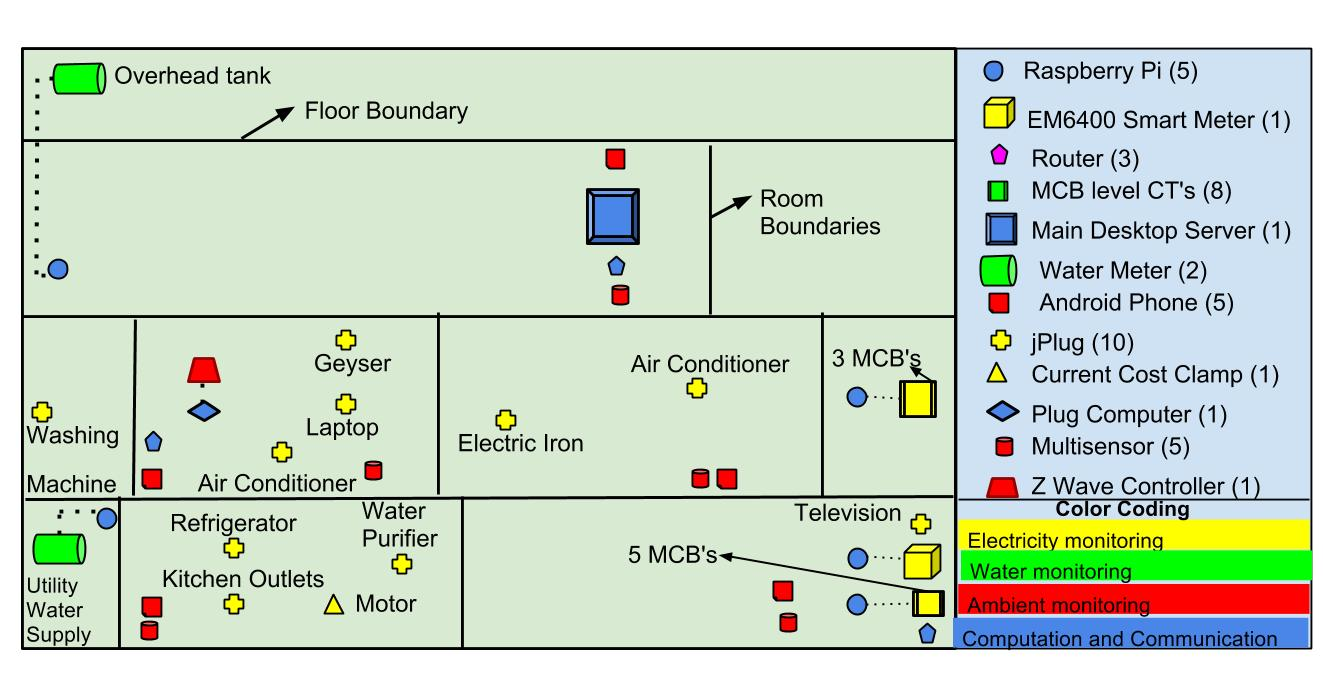
\includegraphics[scale=0.19]{./figures/overall_deployment.jpg}
    \vspace{-6mm}    
    \caption{Schematic showing overall home deployment}   
    \label{fig:overall}
\end{figure}

\subsection{Sensing Infrastructure}
\label{sec:sensing}
For sensing, we took a ``leave no stone unturned'' approach, where  we chose to monitor as many physical parameters (ambient conditions, electricity usage and water usage) and non-physical parameters (such as network strength and network connectivity, among other). We, however, chose to deploy these sensors in a way that home users can continue their daily routines without getting affected. Many of these sensors were procured from outside India due to limited options available in the Indian context. Detailed description of the sensors used for monitoring various parameters are explained next.

\noindent\textbf{Electricity monitoring:} %A typical home electricity setup involves a meter which is installed by utility companies and measures overall electricity usage. Further electric cabling is divided into various Miniature Circuit Breakers (MCB's) which control separate circuits. Typical installations involve putting a separate MCB for each heavy load (such as air conditioners) and clubbing various lights, fans and other smaller loads into separate MCB's. Further each individual appliance is controlled via a switch. There are two types of appliances- i) plug loads like refrigerator and electric iron, which need to be physically ``plugged" into the sockets; ii) loads like lights and fans, which do not need to be ``plugged" in by the user and can directly be switched on or off. We highlight the above described home electricity distribution in \figref{fig:electricity_distribution}. 
We chose to monitor electricity consumption across different resolutions - electricity meter monitoring the consumption at the home aggregate level, Current Transformers (CTs) monitoring current for Miniature Circuit Breakers (MCB's) (each connected to a combination of appliances) and plug level monitors for consumption monitoring of plug load based appliance (see \figref{fig:electricity_distribution} for illustration). 

\begin{enumerate}\denselistbib
\item \textbf{Meter level:} Schneider Electric EM6400\footnote{\url{www.goo.gl/01edPS}} smart meter is used to instrument the main power supply (see \figref{fig:em6400} showing EM6400 smart meter deployed in the electricity panel). %While cheaper variants from the same company were available, we chose to use EM6400 as it also provides reactive power. This additional information has been known to be useful for NILM applications~\cite{hart}. 
30:5 ratio CT was used on the power mains coming from the grid to ensure that the load current is within the permissible limits (5 A) of the meter. All the necessary parameters including voltage, current, frequency, phase angle, and power (apparent, real, reactive) were read at 1 Hz using Modbus over RS485-serial link provided by EM6400. Based on our experience, we believe that the support required for large scale smart metering deployments, exists in the Indian context. 

\item \textbf{Circuit level:} Split CTs, clamped to individual MCB's, are used for monitoring circuit level current. Since no commercial solution is easily available in India for panel level monitoring, a low cost microcontroller platform is used to collect Analog output from CTs at 125 KHz, calculate the rms value and communicate it over serial UART interface (\figref{fig:ct} captures CTs monitoring 3 MCBs on the first floor MCB box).

\item \textbf{Appliance level:} Similar to circuit level monitors, there are no good commercial options for plug level monitors in Indian context as well. Correspondingly, we worked with our collaborators who in-house developed jPlug\footnote{A variant of nPlug~\cite{nplug}} to measure individual appliance power consumption. 9 of these jPlugs were used to monitor plug-load type appliances. jPlug sits in between an appliance and the socket and provides multiple parameters (including voltage, current, phase angle and frequency) at 1 Hz resolution. We also used Current Cost based CT to measure the power consumption for electric motor (used to pump water), which is not a plug-load, yet has significant power consumption (approx. 700 Watts). jPlug and Current Cost CT deployment are shown in \figref{fig:jplug} and \figref{fig:cc} respectively. jPlug makes a HTTP POST connection to log measured parameters. Current Cost exposes apparent power data over the USB port. 
\end{enumerate}

\noindent \textbf{Water monitoring:} There are a few differences in home water distribution in India when compared to developed countries. Due to non availability of 24x7 water supply, overhead water tanks (typically 1000 liters capacity) are used to store water, when available, and supply it for home activities throughout the day. Due to low water pressure, even during the times when the supply is available, electric motors are used to pump the water for storage. %Thus, the flow of water in a home can be summarized as follows: 1) Water from utility comes to the home; 2) Electric motor is used to aid in pumping the water up to the tank; 3) Water flows downward from the tank whenever water is consumed. 
\figref{fig:water_distribution} illustrates the water flow distribution, together with placement of water meters. One water meter is placed at the inlet (coming from the utility) and another one at the outlet from the water tank (flowing downwards) to capture the incoming (from utility) and outgoing (from tank) water consumption. 

Due to prohibitive cost and difficulty in procurement of digital water meters in India, we chose to use Zenner Aquamter's multijet\footnote{\url{www.aquametwatermeters.com/multijet.html}}, a pulse output based water meters. Output pulse is generated through a 4-20 mA current loop, commonly used for analog signaling in industrial process control instruments. For the water meter connected to the utility, over a 0.5 inch diameter pipe, a pulse is generated for every 1 liter of water consumption. Water meter connected to the outlet of stoarge tank, with 1.25 inch diameter, generates a pulse every 10 liters of water consumption. %generating a pulse every few liters. The precision is based on the quality of the sensor and the diameter of the water pipe. The water meter we used for overhead tank gives a pulse every 10 liters, whereas the one used for inlet supply from utility gives a pulse every 1 liter. These pulses can be measured using the circuit diagram for 4 ma loop shown in ... 
\figref{fig:water_meter} shows the water meter deployed inline at the overhead tank.

\noindent \textbf{Ambient conditions monitoring:} We used ZWave based HomeSeer HSM100\footnote{\url{www.homeseer.com/pdfs/guides/HSM100_Release_Notes.pdf}} multisensors for monitoring motion, light and temperature across 5 rooms in the home. Till date, to the best of our knowledge, no commercial ZWave based sensor is available working on Indian frequency (865.2 MHz). We correspondingly imported EU frequency (868.4 MHz) devices and used it for ambient monitoring. For these HSM100, motion is reported in an event-driven manner (i.e. whenever there is change in motion status, a reading is reported) and temperature and light are polled at 1 Hz. We also placed 1 Android phone at a fixed location in each room and ran FunF journal application\footnote{\url{http://www.funf.org/journal.html}} to log ambient parameters such as light and sound level every 30 seconds for 5 seconds.

\noindent \textbf{Miscellaneous:} Android phones, in addition to measuring ambient conditions, were also used to scan and log Bluetooth, WiFi and GSM networks. All home occupants were requested to keep the Bluetooth on during the duration of the experiment. The network scanning was done every 1 minute and is stored locally on the SD card. External weather conditions, such as temperature, humidity and wind speed, were also logged every 10 minutes using publicly available API's from weather monitoring stations\footnote{Forecast, World Weather, Open Weather Map}.
%\footnote{Forecast: \url{www.forecast.io}, World Weather: \url{www.worldweatheronline.com}, Open Weather Map: \url{www.openweathermap.org}}
Additionally, network traffic was sensed to monitor connectivity and signal strength. Such miscellaneous data collection, together with detailed electrical consumption, water consumption and ambient information, can be used for multiple applications including energy-apportionment (i.e. assigning energy usage to different occupants within the home), localization and correlating energy usage with outside temperature.

\noindent Complete sensing infrastructure is summarized in \tabref{tab:sensing}.


\begin{table*}
\caption{Sensing Infrastructure}

\label{tab:sensing}
\tabcolsep=0.015cm
\begin{tabular}{|l|l|l|l|l|l|l|}
\hline
Sensor&Sensor&Sampling&Resolution&Qua-&Commu-&Observed\\
name&type&frequency&&ntity&nication&parameters\\
&&(Hz)&&&&\\
\hline

EM6400&Electric Meter&1&Home&1&RS 485 Serial&Voltage, Current, Frequency,\\ 
&&&&&&Phase, Power(Active, Reactive \\ 
&&&&&&and Apparent), Energy\\ \hline
Aquamet &Water Meter&5&Main supply&2&Direct wire con-&10 liter events for tank and \\ 
multijet&&& and tank&&nection to GPIO&1 liter events for main supply\\ \hline
Homeseer &Ambient multisensor&Light, temperature: 1&Room &6&ZWave&Light, temperature\\ 
     HSM100           &&PIR: event based&&&& and motion\\ \hline
Android&Ambient multisensor&Audio, light: Reading is &Room&5&Manually&Audio features, light, nearby \\ 
phones&and network&taken for 5 seconds, every 30 &&&transfer files&bluetooth, cell-tower, WiFi\\ 
&&seconds; Nearby WiFi, cellular&&&to PC&\\ 
&&, bluetooth: 1/60&&&&\\ \hline
Prototype CT&Electricity meter&20&MCB&8&Serial&RMS Current \\\hline
jPlug&Electricity meter & 1 &Appliance&10&WiFi&Voltage, Current, Frequency,\\ 
&&&&&&Power (Active and Apparent),\\
&&&&&& Energy, Phase\\ \hline	
Current Cost&Electricity meter&1/6&Appliance&1&Serial&Apparent power\\ \hline


\end{tabular}


\end{table*}

\subsection{Communication and Computation Infrastructure}
Multitude of sensing infrastructure, as described in \secref{sec:sensing}, involves multitude of communication channels as well. Different computing platforms - microcontrollers, Single Board Computers (SBCs) (e.g. Raspberry Pi\footnote{\url{www.raspberrypi.org}} (RPi) and Ionics Stratus\footnote{\url{www.ionics-ems.com/plugtop/stratus.html}}) and desktops are used for data collection.  
%In our experience we found that using a desktop computer for collecting data from individual sensors would be an overkill in terms of cost, processing power and physical space used. Although microcontrollers are cheap and occupy little space, they do not expose enough abstractions for high level programming, are often difficult to debug and are inherently hard to multi task. We thus decided to use Single Board Computers (SBC's) for sensor data collection. We used Raspberry Pi\footnote{\url{www.raspberrypi.org}} (RPi) and Ionics Stratus\footnote{\url{www.ionics-ems.com/plugtop/stratus.html}} based SBC's. 
SBCs served as a good low cost alternative (25 \$) constituting 700 MHz ARM processors, support for Linux based distributions and allow for coding in higher level languages such as Python. %These SBC's run from SD cards whose size can be chosen as per requirement. 

We used 5 RPi and 1 Ionics Stratus plug computer in our deployment. We used a 2 GHz Desktop PC running Linux, as the main server where all the data was stored. %The software stack running on the SBC's and how they interacted with the main server and collected data from different sensors is described below:
One RPi was connected to EM6400 using RS485-USB converter. We developed a custom Python program based on pyModbus\footnote{\url{www.github.com/bashwork/pymodbus}} to collect the desired parameters. %library which would serially read 80 registers, using Modbus protocol, to compute 40 electrical parameters as described in \tabref{tab:sensing}. 
All the collected parameters, together with the UTC timestamp is stored in a local CSV file. A new CSV was created every 15 minutes. A background program would periodically try to upload CSV files older than 15 minutes, to the main server, where the data is pushed in MySQL database. This architecture for data collection - creating a new CSV periodically, uploading older CSV periodically to main server where the data is then pushed into MySQL, is used for all of our sensors connected to SBCs. We call this model \paradigms and describe it in more details in section \secref{sec:architecture}. On similar lines, USB output from Current Cost (providing data in xml format) is received on another RPi and goes through the \paradigms architecture for data collection. %A custom Python script will store data in CSV files every 15 minutes which is then uploaded by a separate background script. 
Although Current Cost has its own cloud based API's, we chose to collect data from it locally, in order to avoid data losses occurring due to network failures. 

%\noindent \textbf{Current Cost data collection:} Although Current Cost has its own cloud based API's, we chose to collect data from it locally, in order to avoid data losses occurring due to network failures. Current Cost provides power data in xml format over the serial interface. We thus connected the USB cable-out from the Current Cost receiver to RPi and wrote a simple Python script to read data serially using pySerial\footnote{\url{www.pyserial.sourceforge.net}} and store it in a CSV file along with UTC timestamp. CSV creation and uploading to central server was done in a similar fashion as was done for EM6400.

Two RPi were used to connect to the microcontroller based circuit monitor to read the data over the serial port and process it further using \paradigm. One of the RPi connected to the meter was used for circuit monitoring as well for the CTs used in the same panel. GPIO headers on two more RPis were used to interface with each water meter respectively for collecting pulse output over the 4-20 mA current loop interface. We initially wrote an interrupt driven program in Python to detect 10 liter and 1 liter events for the tank and supply water meters respectively. We observed that noise introduced in the circuit due to long cable lengths led to a lot of false events. Correspondingly, we modified our program and polled at a frequency of 5 Hz to obtain GPIO status and further processed this data using \paradigm.	 
%\noindent \textbf{MCB data collection:} Our custom built CT based monitor for collecting current data from different MCB's exposes data serially which is read using pySerial on a RPi and processed further using \paradigm.

Data from jPlugs (using the HTTP post request every second) is directly collected on the server machine where a web daemon listened to requests from jPlug and dumped them in MySQL. Ionics Plug Computer is used to collect data from all ZWave based sensors. We wrote custom wrappers around OpenZWave\footnote{\url{www.code.google.com/p/open-zwave}} to collect temperature and light information on per second basis, and motion information based on events. A ZWave controller was connected over USB with Ionics and the data was processed further using \paradigm. \figref{fig:plug} shows the plug computer collecting ambient sensor data from ZWave controller. A manual dump of locally collected data on each Android phone was performed every 15 days. Electricity failure and unreliable internet are well known problems in India and are highlighted in \secref{sec:learning}. Owing to these problems, we chose to collect weather data from 3 different weather stations, in one of the servers hosted by our collaborators in the USA. 


%\noindent \textbf{jPlug appliance data collection:} jPlug makes a HTTP post every second with upto 10 electrical parameters. We saved this data directly on the server machine where a web daemon listened to requests from jPlug and dumped them in MySQL.

%\noindent \textbf{Water data collection:} Based on circuitry explained in \secref{sec:sensing}, we used GPIO header on RPi and wrote an interrupt driven program in Python to detect 10 liter and 1 liter events for the tank and supply water meters respectively. We found that noise introduced in the circuit due to long cable lengths led to a lot of false events. Thus, we modified our program and polled at a frequency of 5 Hz to obtain GPIO status and further processed this data using \paradigm.	

%\noindent \textbf{Homeseer HSM100 data collection:} We wrote custom wrappers around OpenZWave\footnote{\url{www.code.google.com/p/open-zwave}} program to collect temperature and light information on a per second basis, and motion information based on events. ZWave controller which controls all the ZWave based sensors was connected to the plug computer over USB. Data was processed further using \paradigm. \figref{fig:plug} shows plug computer collecting ambient sensor data from ZWave controller.

%\noindent \textbf{Android data collection:} We used FunF journal which would store data inside phone's SD card. We would take a dump once every 15 days and empty the SD card for further data collection.


A lot of issues, pertaining to SBCs, were observed in our deployment. As an example, the OpenZWave program that we used created log files for its own diagnostics, that eventually consumed the 512 MB flash drive space on the plug computer. This was fixed eventually by deleting older logs. Such problems encouraged us to develop soft-sensor streams, whereby we collected hard disk space, ping success, CPU utilized, remaining RAM space and temperature of the processor, for all the computing devices including the server at regular intervals. These soft-sensor streams can be used for offline analysis as well as for real time alerting and fault diagnosis. Similar soft-sensor streams have also been used in the previous work~\cite{hitchhiker_residential} for raising alerts.

Similar to prior research, reporting WiFi discontinuity in homes in the USA~~\cite{hitchhiker_residential}, we also observed that one WiFi router will not suffice for our 3 storey home. We thus used 3 Netgear JNR1010\footnote{\url{www.support.netgear.com/product/JNR1010}} routers, where the router on the first floor acted as the host and the routers on the ground and the second floor were bridged to it. More details regarding the need of multiple routers and network availability in homes is described in \secref{sec:learning} and \secref{sec:common}.


\subsection{System Architecture}	
\label{sec:architecture}
Various middleware systems such as sMAP~\cite{smap}, Building Depot~\cite{buildingdepot} and SensorAct~\cite{Arjunan12} have been proposed in the past for sensor data collection. However, we found that they are not fine tuned to our needs arising from faulty internet, power failures, etc. Based on our experience and previous work~\cite{hitchhiker_residential}, where importance of simplifying the architecture are proposed, we propose \paradigm. \paradigms involves two main ideas- local storage (on SBCs) and periodic data upload (from SBC to server, and from server to cloud). As explained above, we used SBCs to collect data from sensors. This data was \textbf{locally stored} in form of comma separated value files (CSV) and was \textbf{periodically uploaded} to the main desktop server. In case the upload failed, it was retried the next time again. Each SBC had sufficient flash based local storage to accommodate sensor data for a few days, in case there was persistent upload failure.

\begin{figure}     
    \centering 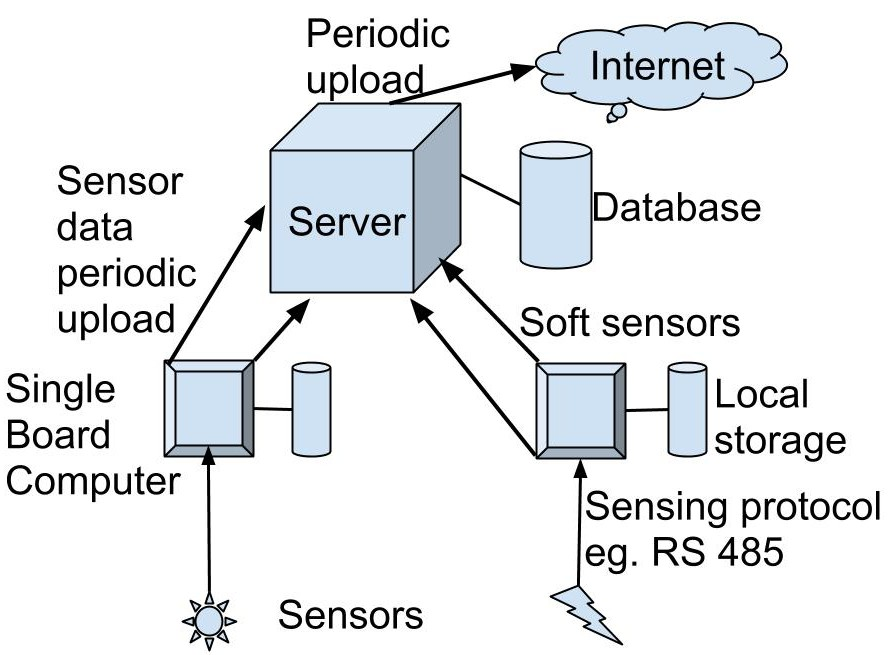
\includegraphics[scale=0.13]{./figures/architecture.jpg}    
    \caption{\paradigm}   
    \label{fig:architecture}   
\end{figure}

\begin{figure}  
\subfloat[\scriptsize Different resolutions of measuring electricity consumption in home: meter, circuit and appliance]{
	 \label{fig:electricity_distribution}
    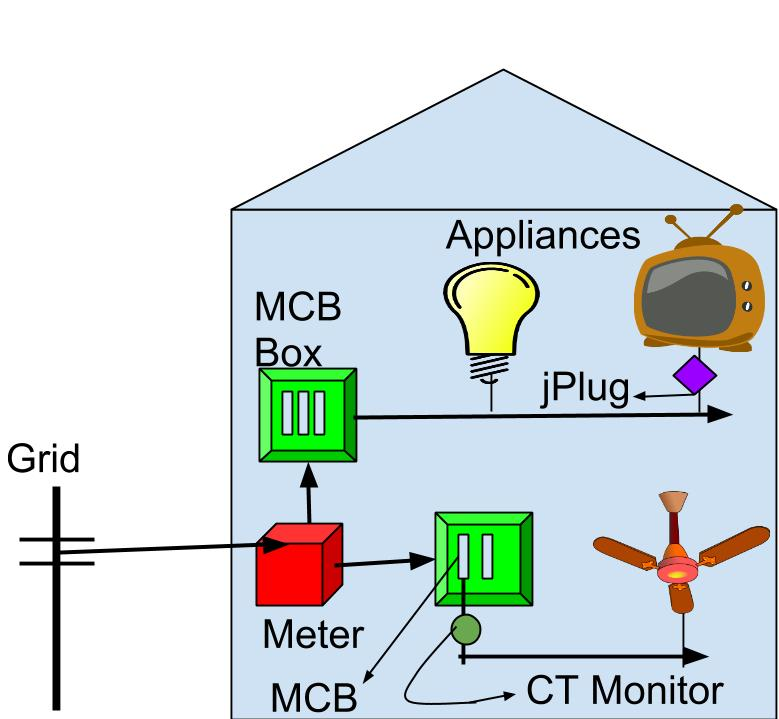
\includegraphics[scale=0.14]{./figures/electricity_distribution.jpg}}
    \hspace{1mm}
    \subfloat[\scriptsize Different resolutions of measuring water consumption in home: inlet supply from utility, outlet supply from tank]{
    	 \label{fig:water_distribution}
        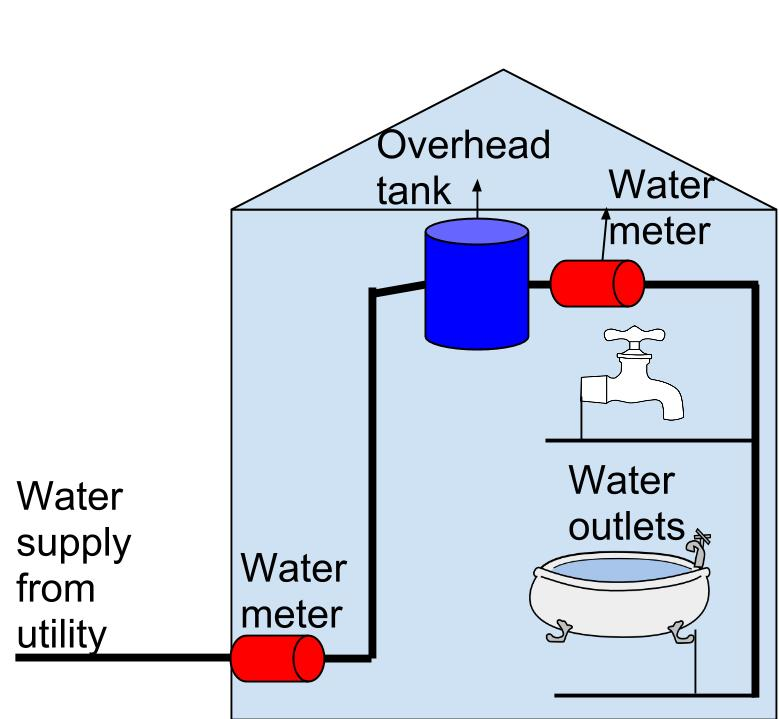
\includegraphics[scale=0.14]{./figures/water_distribution.jpg}}
    \caption{Electricity and water flow inside a home and different resolutions at which these parameters can be monitored}   
      
\end{figure}



Web applications running on the server allowed a home user to locally visualize her data from multiple sensing streams. Further, data from the server can be copied to cloud based servers, such as Dropbox, where applications such as analytics, alerts can be done, allowing outside users and specifically researchers to remotely keep an eye on the deployment. \figref{fig:architecture} explains \paradigms architecture. The salient features of our architecture are as follows:
\begin{itemize}
\item \textbf{Decoupled sensing and data uploading:} This ensures that an error in data uploading does not have an impact on sensing and vice versa. Thus, there is no data loss owing to internet failure. The design choice of decoupling comes from the well established principles of software engineering.
\item \textbf{Minimal internet requirement:} Internet is required \textbf{only} when outside researchers wish to view and analyze collected data in near realtime. Internet failure does not have any impact on sensor data collection. Also, the periodic nature of our uploads ensures that whenever internet is back, data would be uploaded. Further, there is no data loss even if the server goes down for some time, due to local storage.
\item \textbf{Reduced load on server:} Since data is uploaded periodically in larger chunks rather than sending data for each sensor packet, computation and bandwidth requirements on SBCs and server are reduced. Though this comes at the cost of increased storage requirements on SBCs, we found that for all practical purposes, we did not need to provision for more than 1 GB.
\end{itemize}

\begin{figure*} 
    
    \subfloat[\scriptsize EM6400 Smart Meter]{
    \label{fig:em6400}
    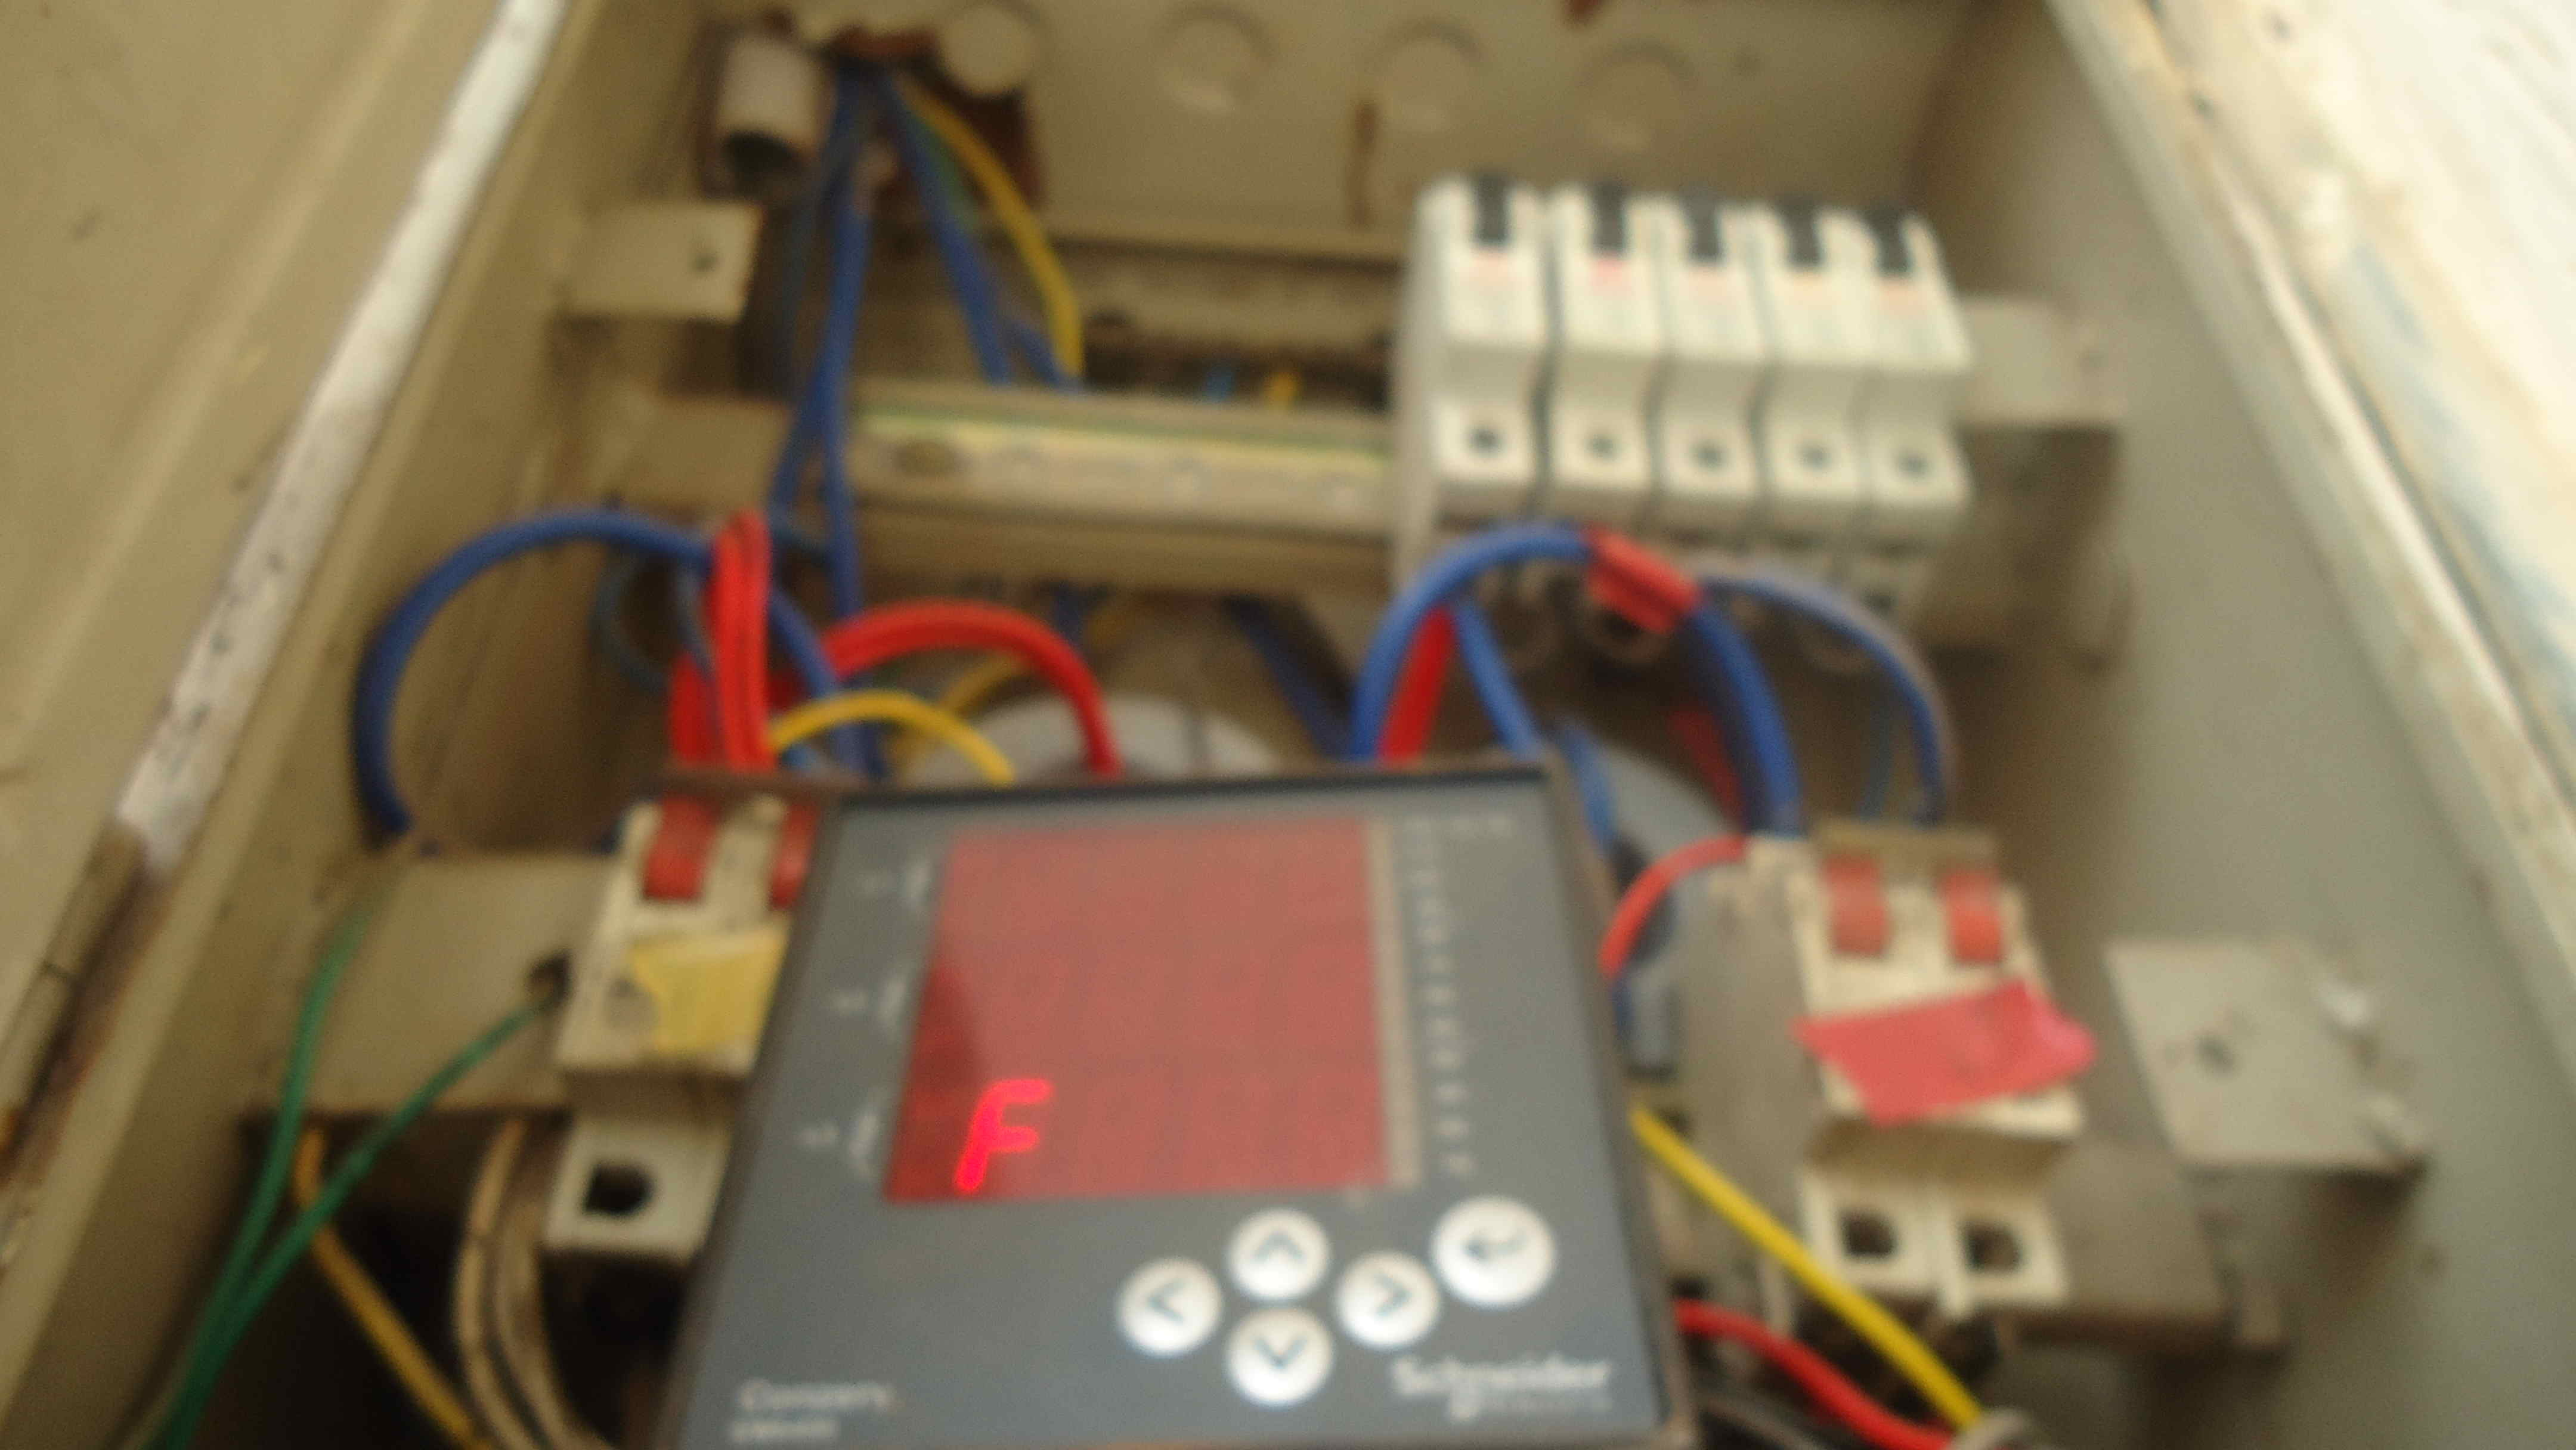
\includegraphics[scale=0.027]{./figures/electric_meter_2.jpg}}
    \hspace{1mm}
     \subfloat[\scriptsize In-house developed CT monitoring system for measuring current data from MCB's]{
        \label{fig:ct}
        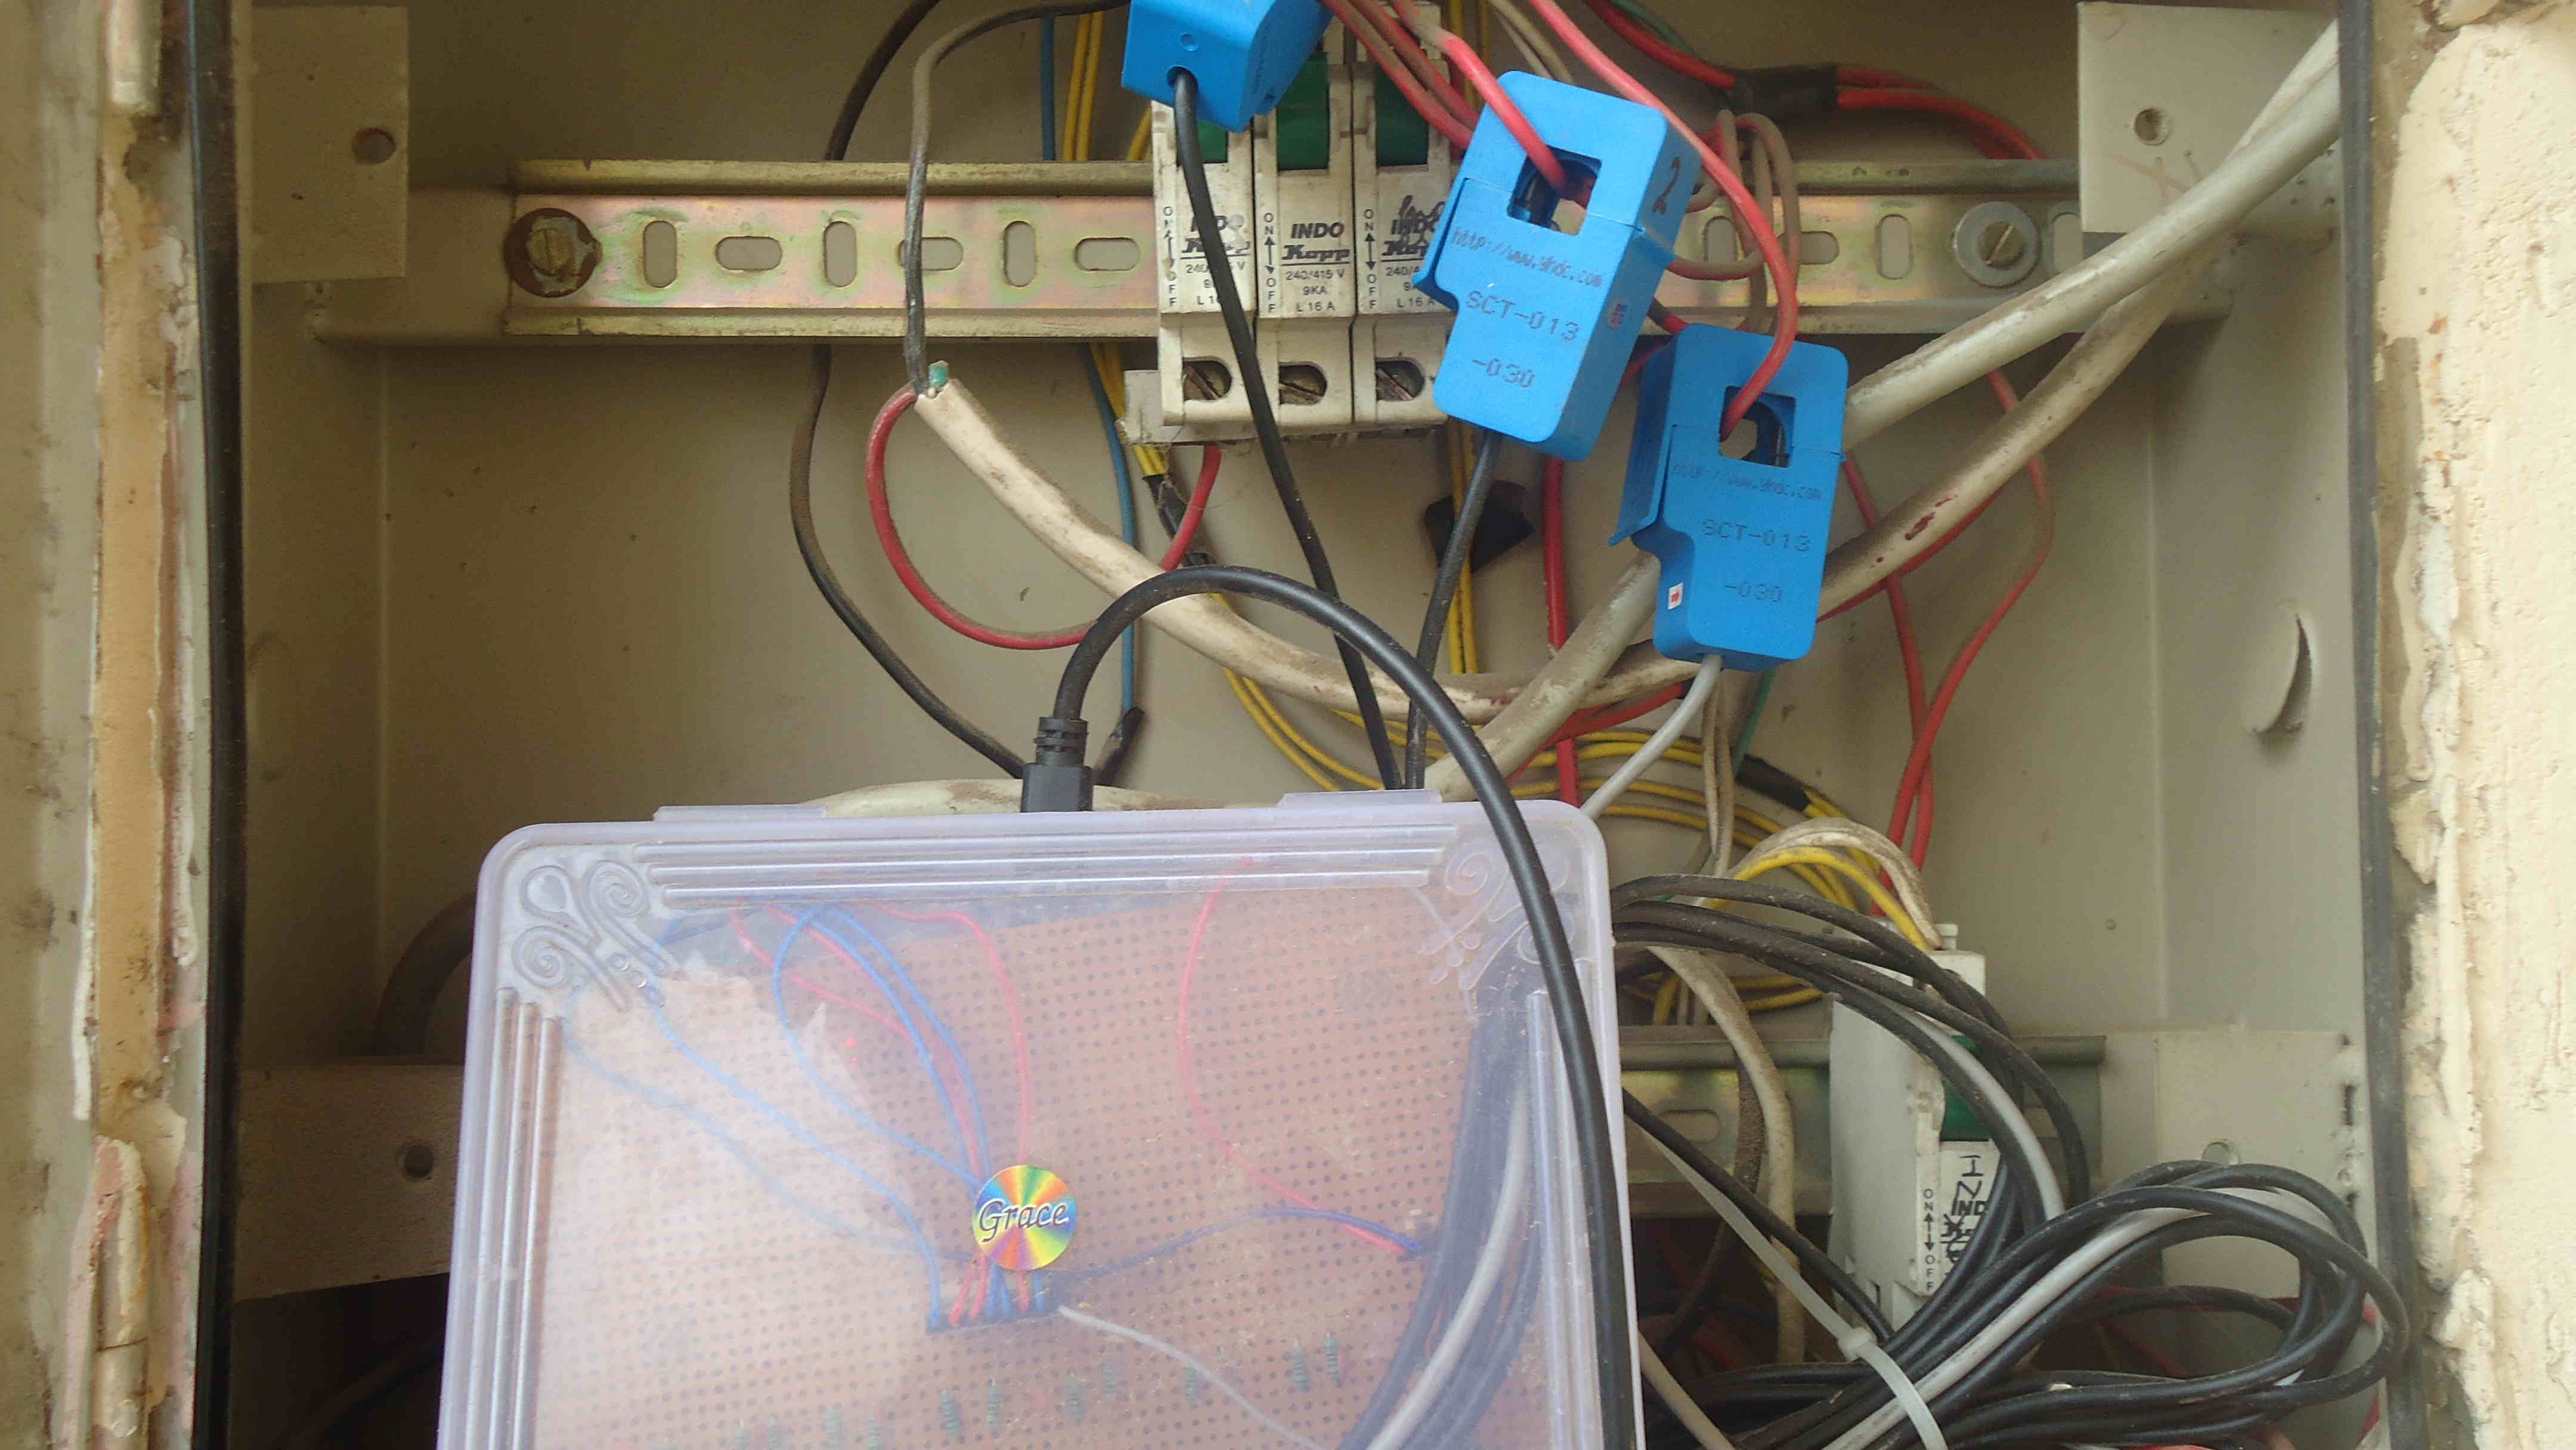
\includegraphics[scale=0.027]{./figures/mcb.jpg}}
       \hspace{1mm}
     \subfloat[\scriptsize Appliance level monitoring using jPlug]{
             \label{fig:jplug}
             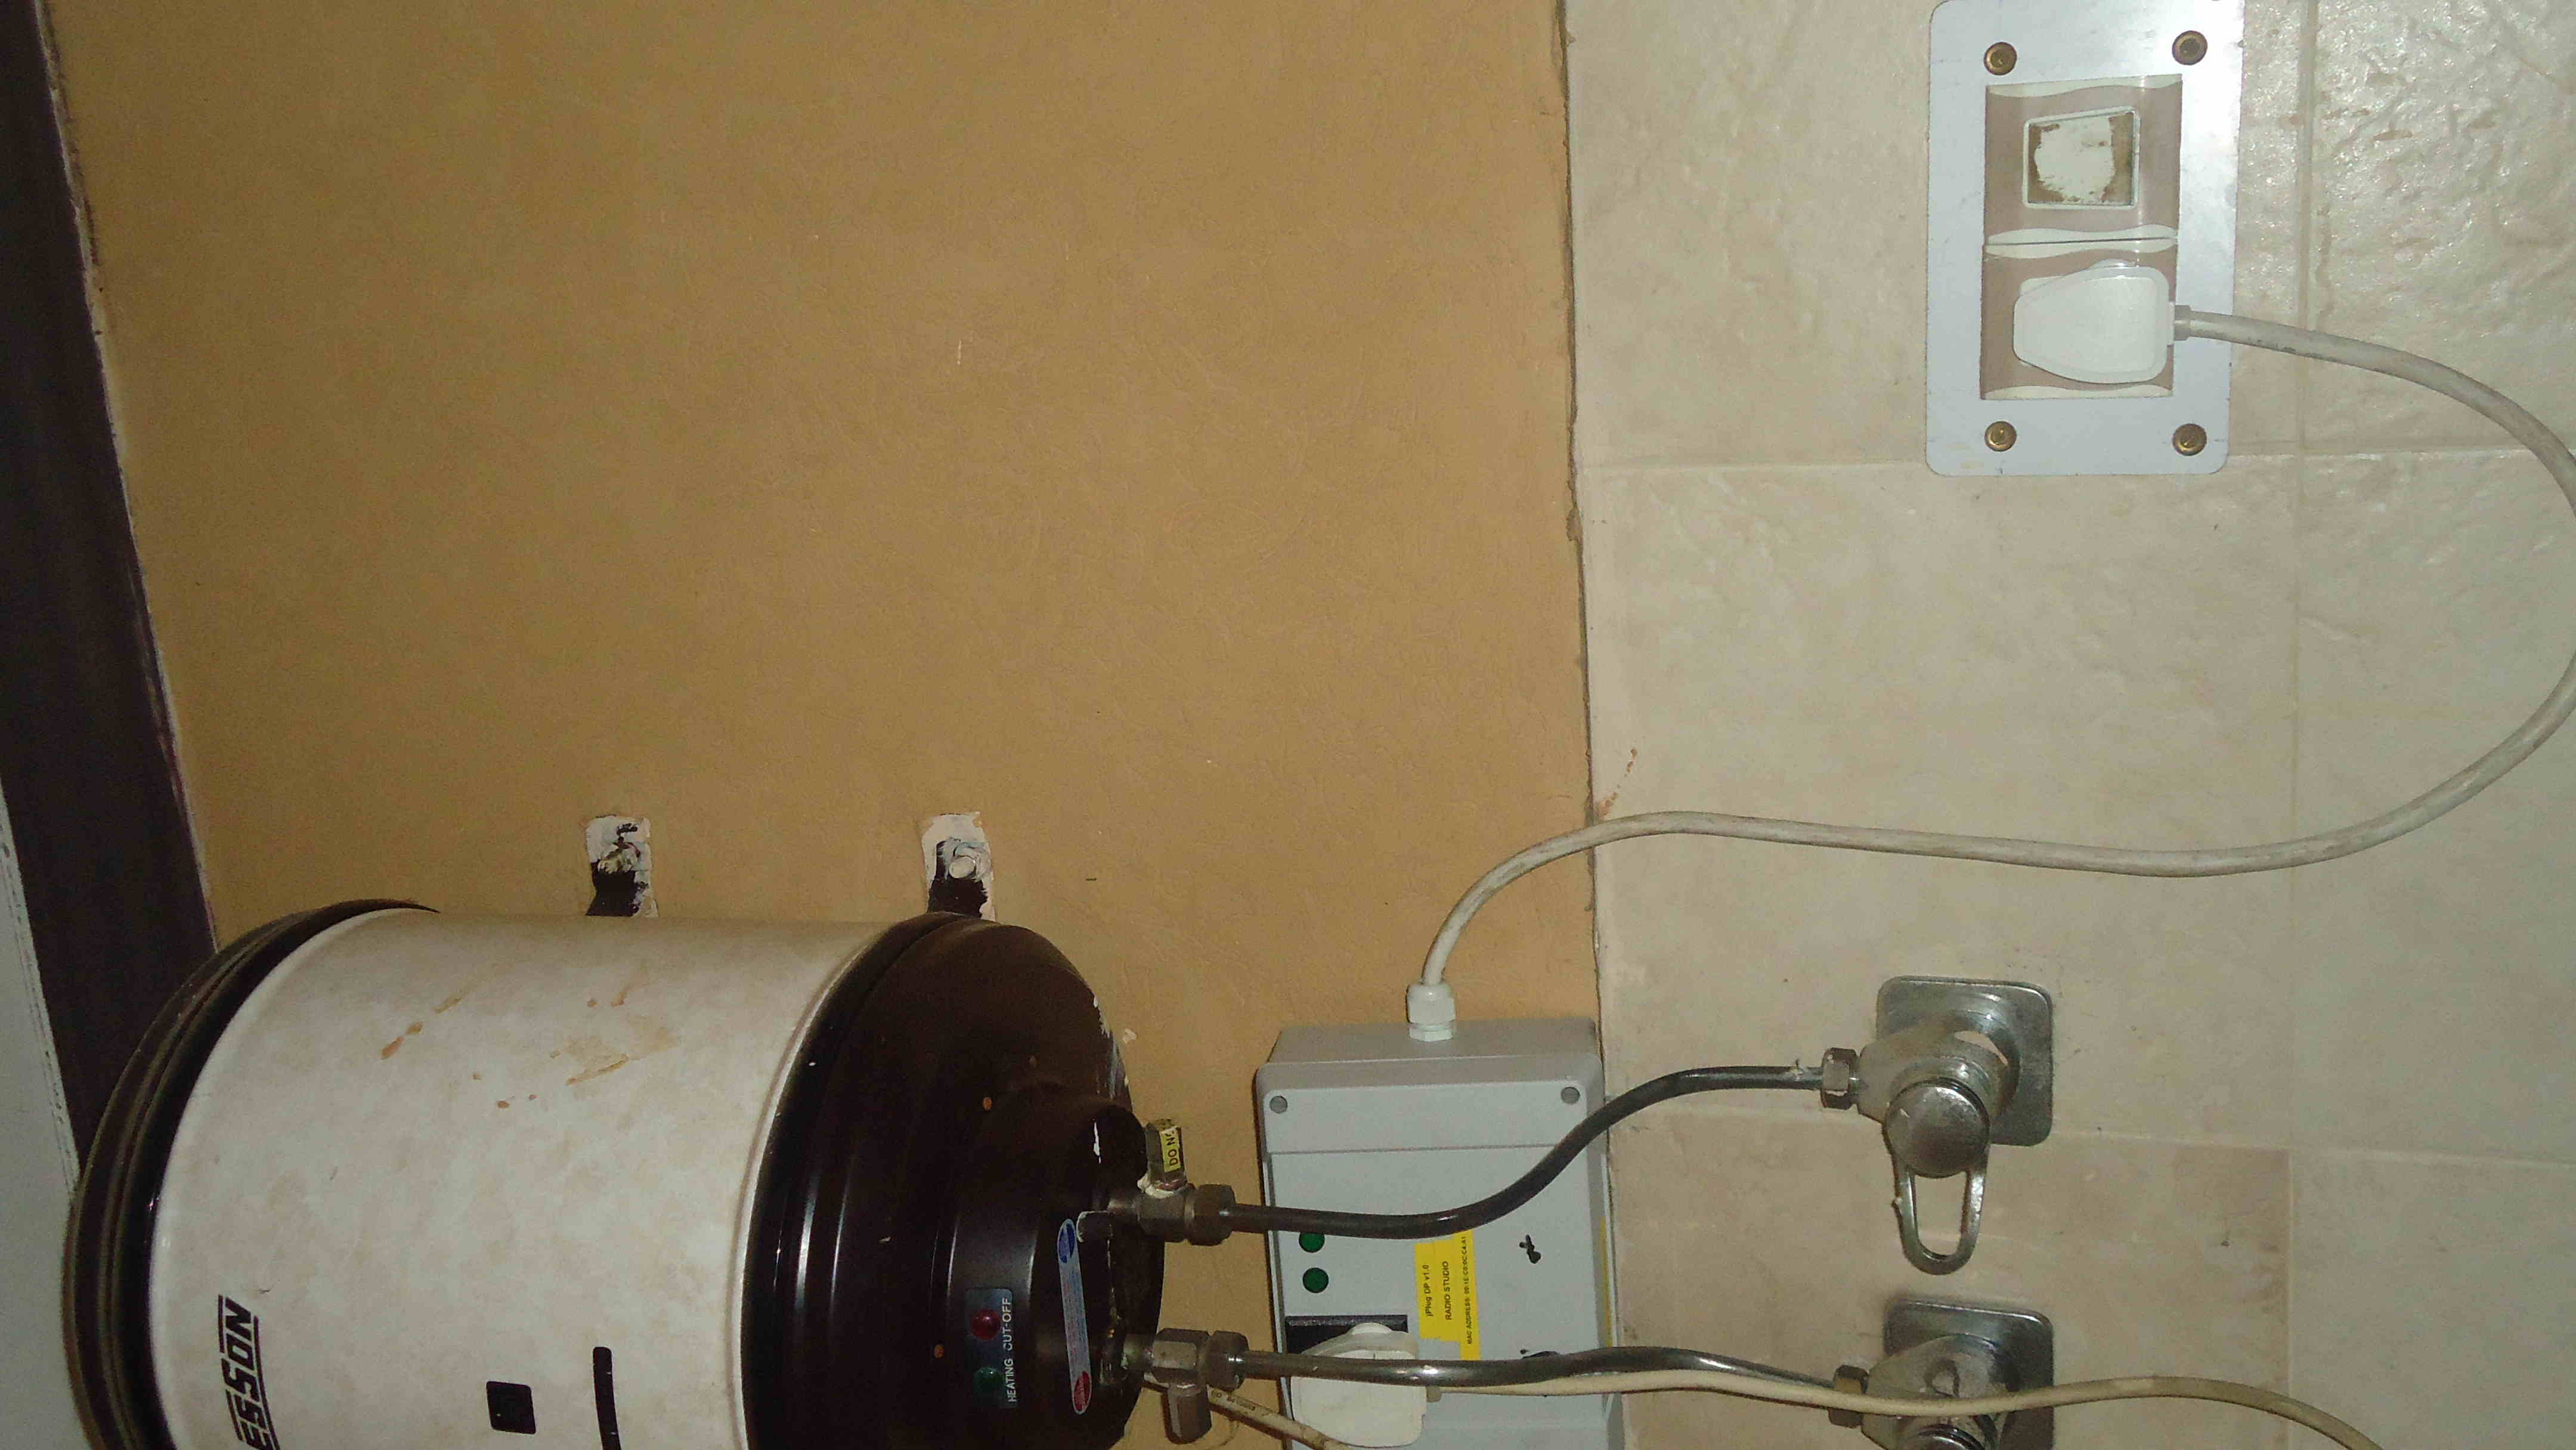
\includegraphics[scale=0.027]{./figures/jplug.jpg}}
             \hspace{1mm}
          \subfloat[\scriptsize Appliance level monitoring using Current Cost CT]{
                  \label{fig:cc}
                  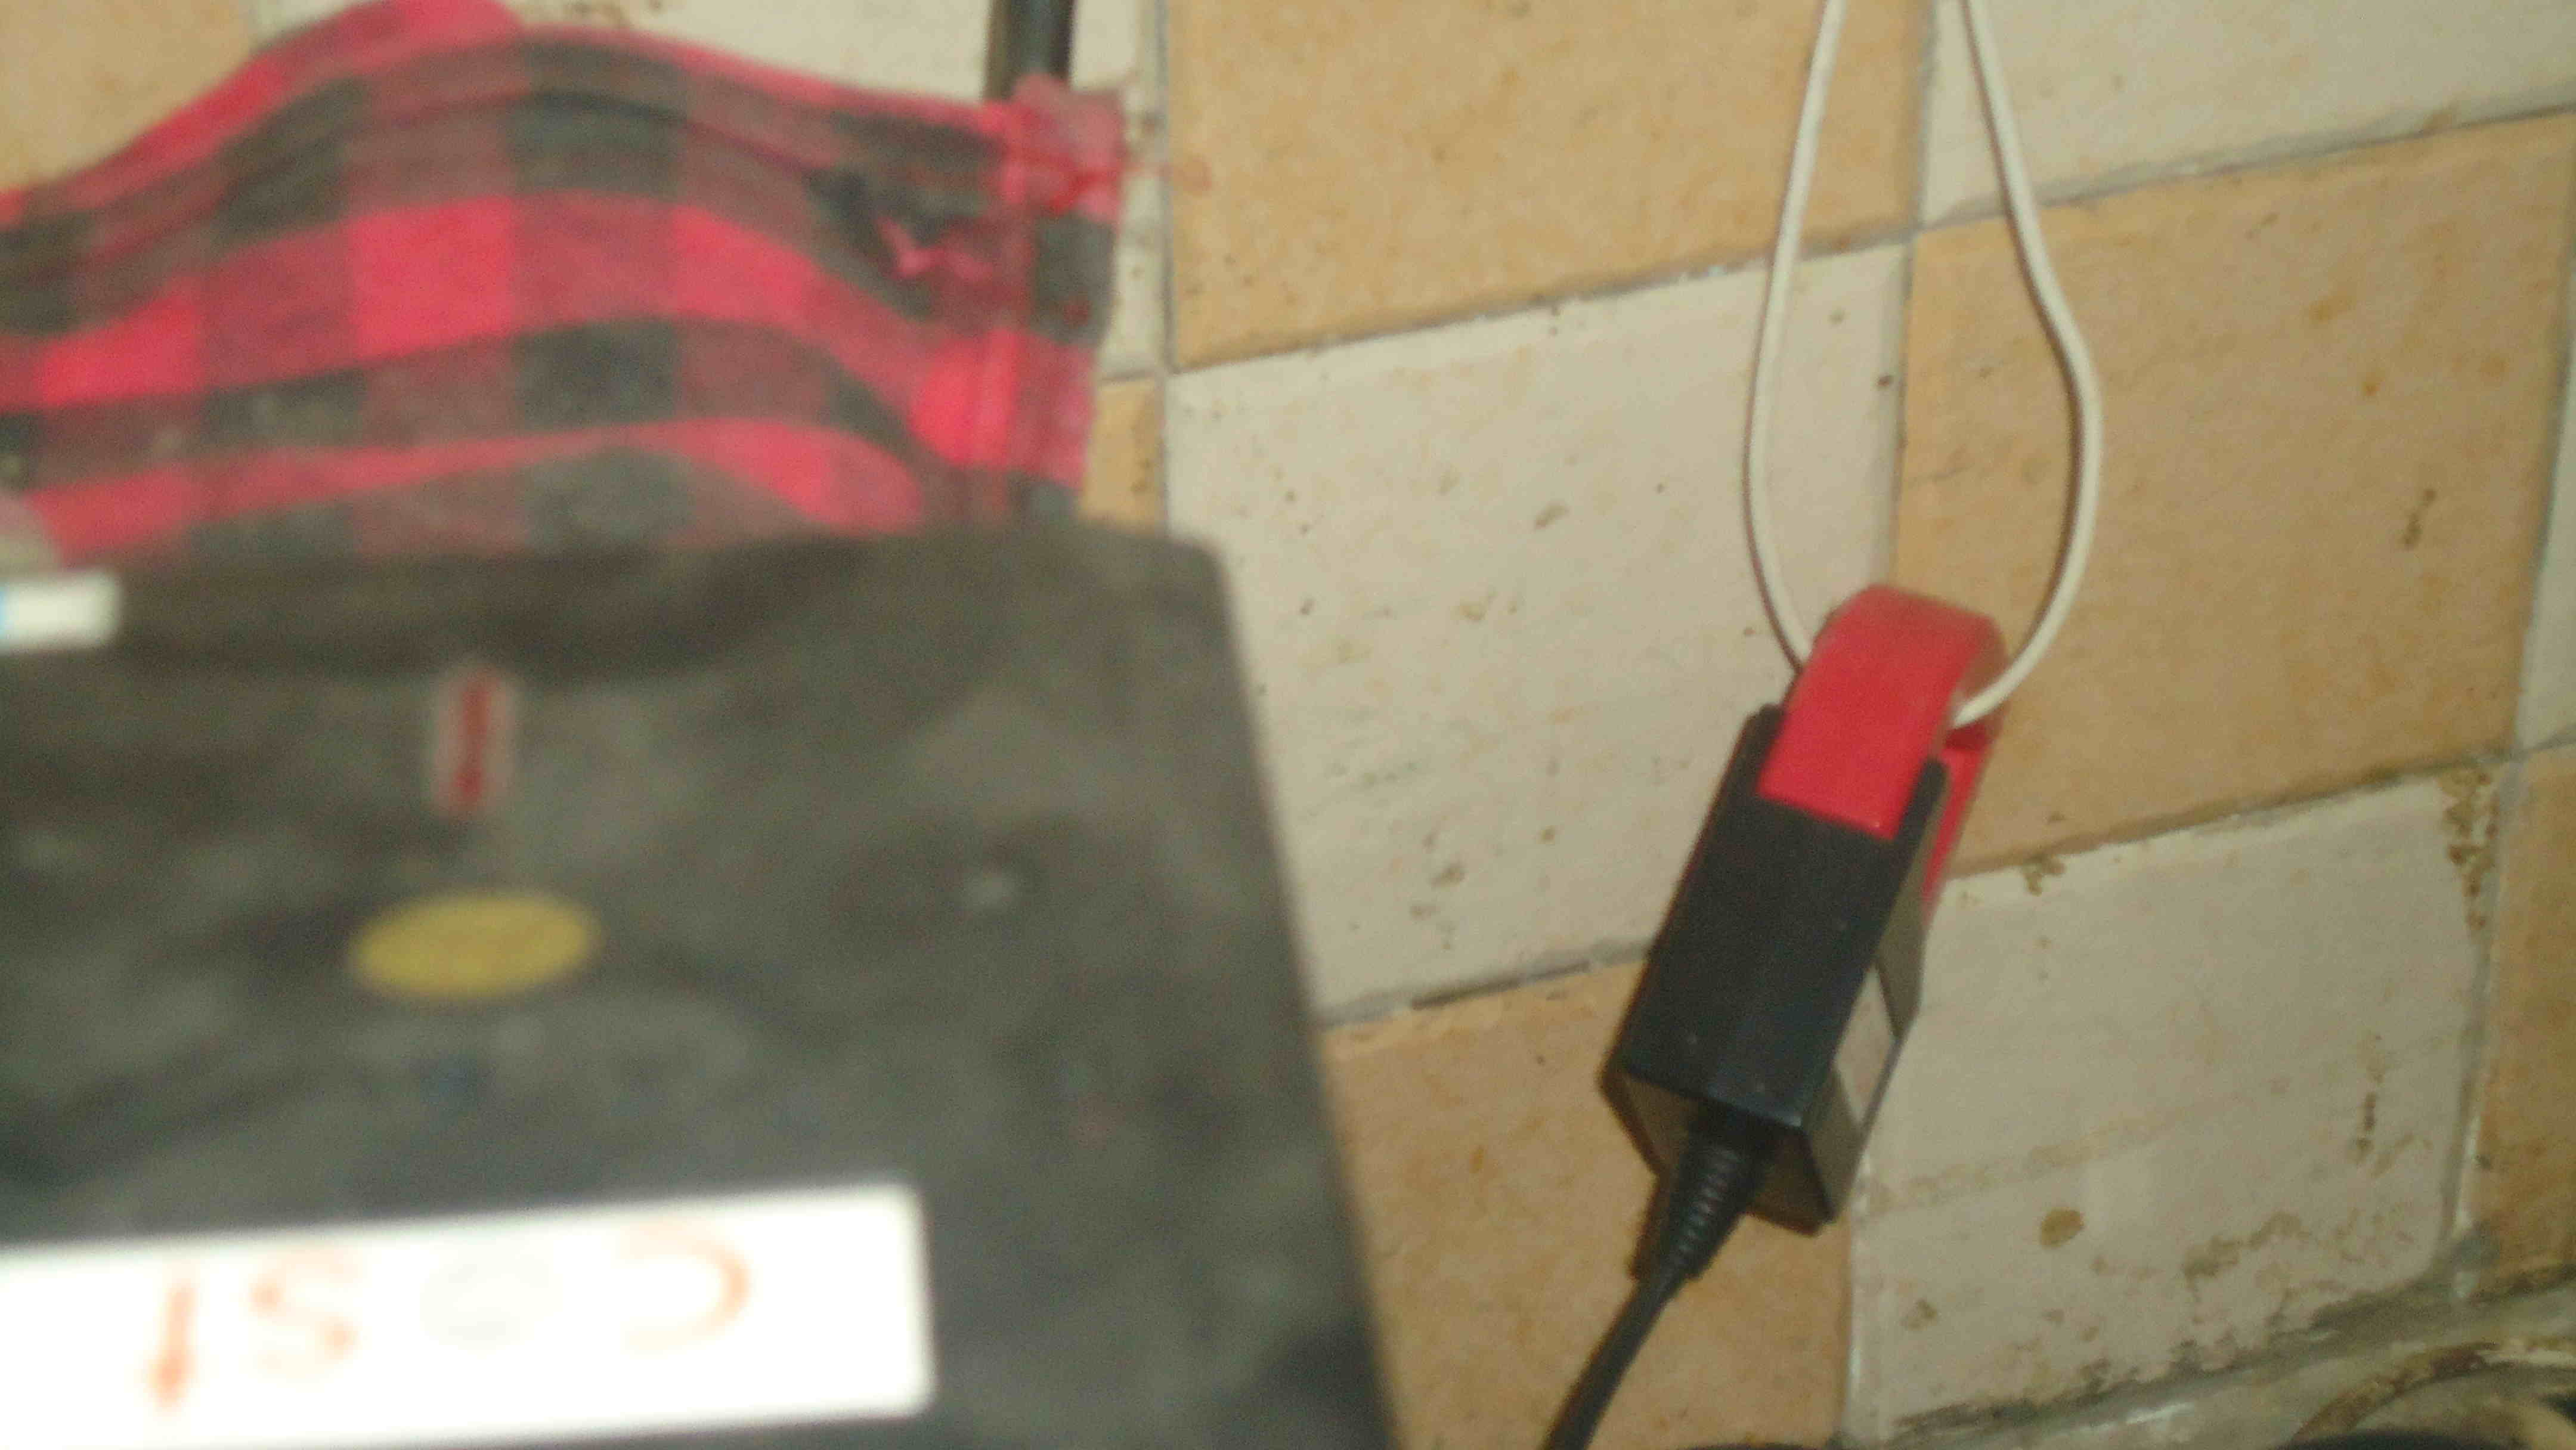
\includegraphics[scale=0.027]{./figures/cc.jpg}}
    %\hspace{0.02\columnwidth}
    \newline
    \vspace{-2mm}
    \subfloat[\scriptsize Water Meter]{
    \label{fig:water_meter}
        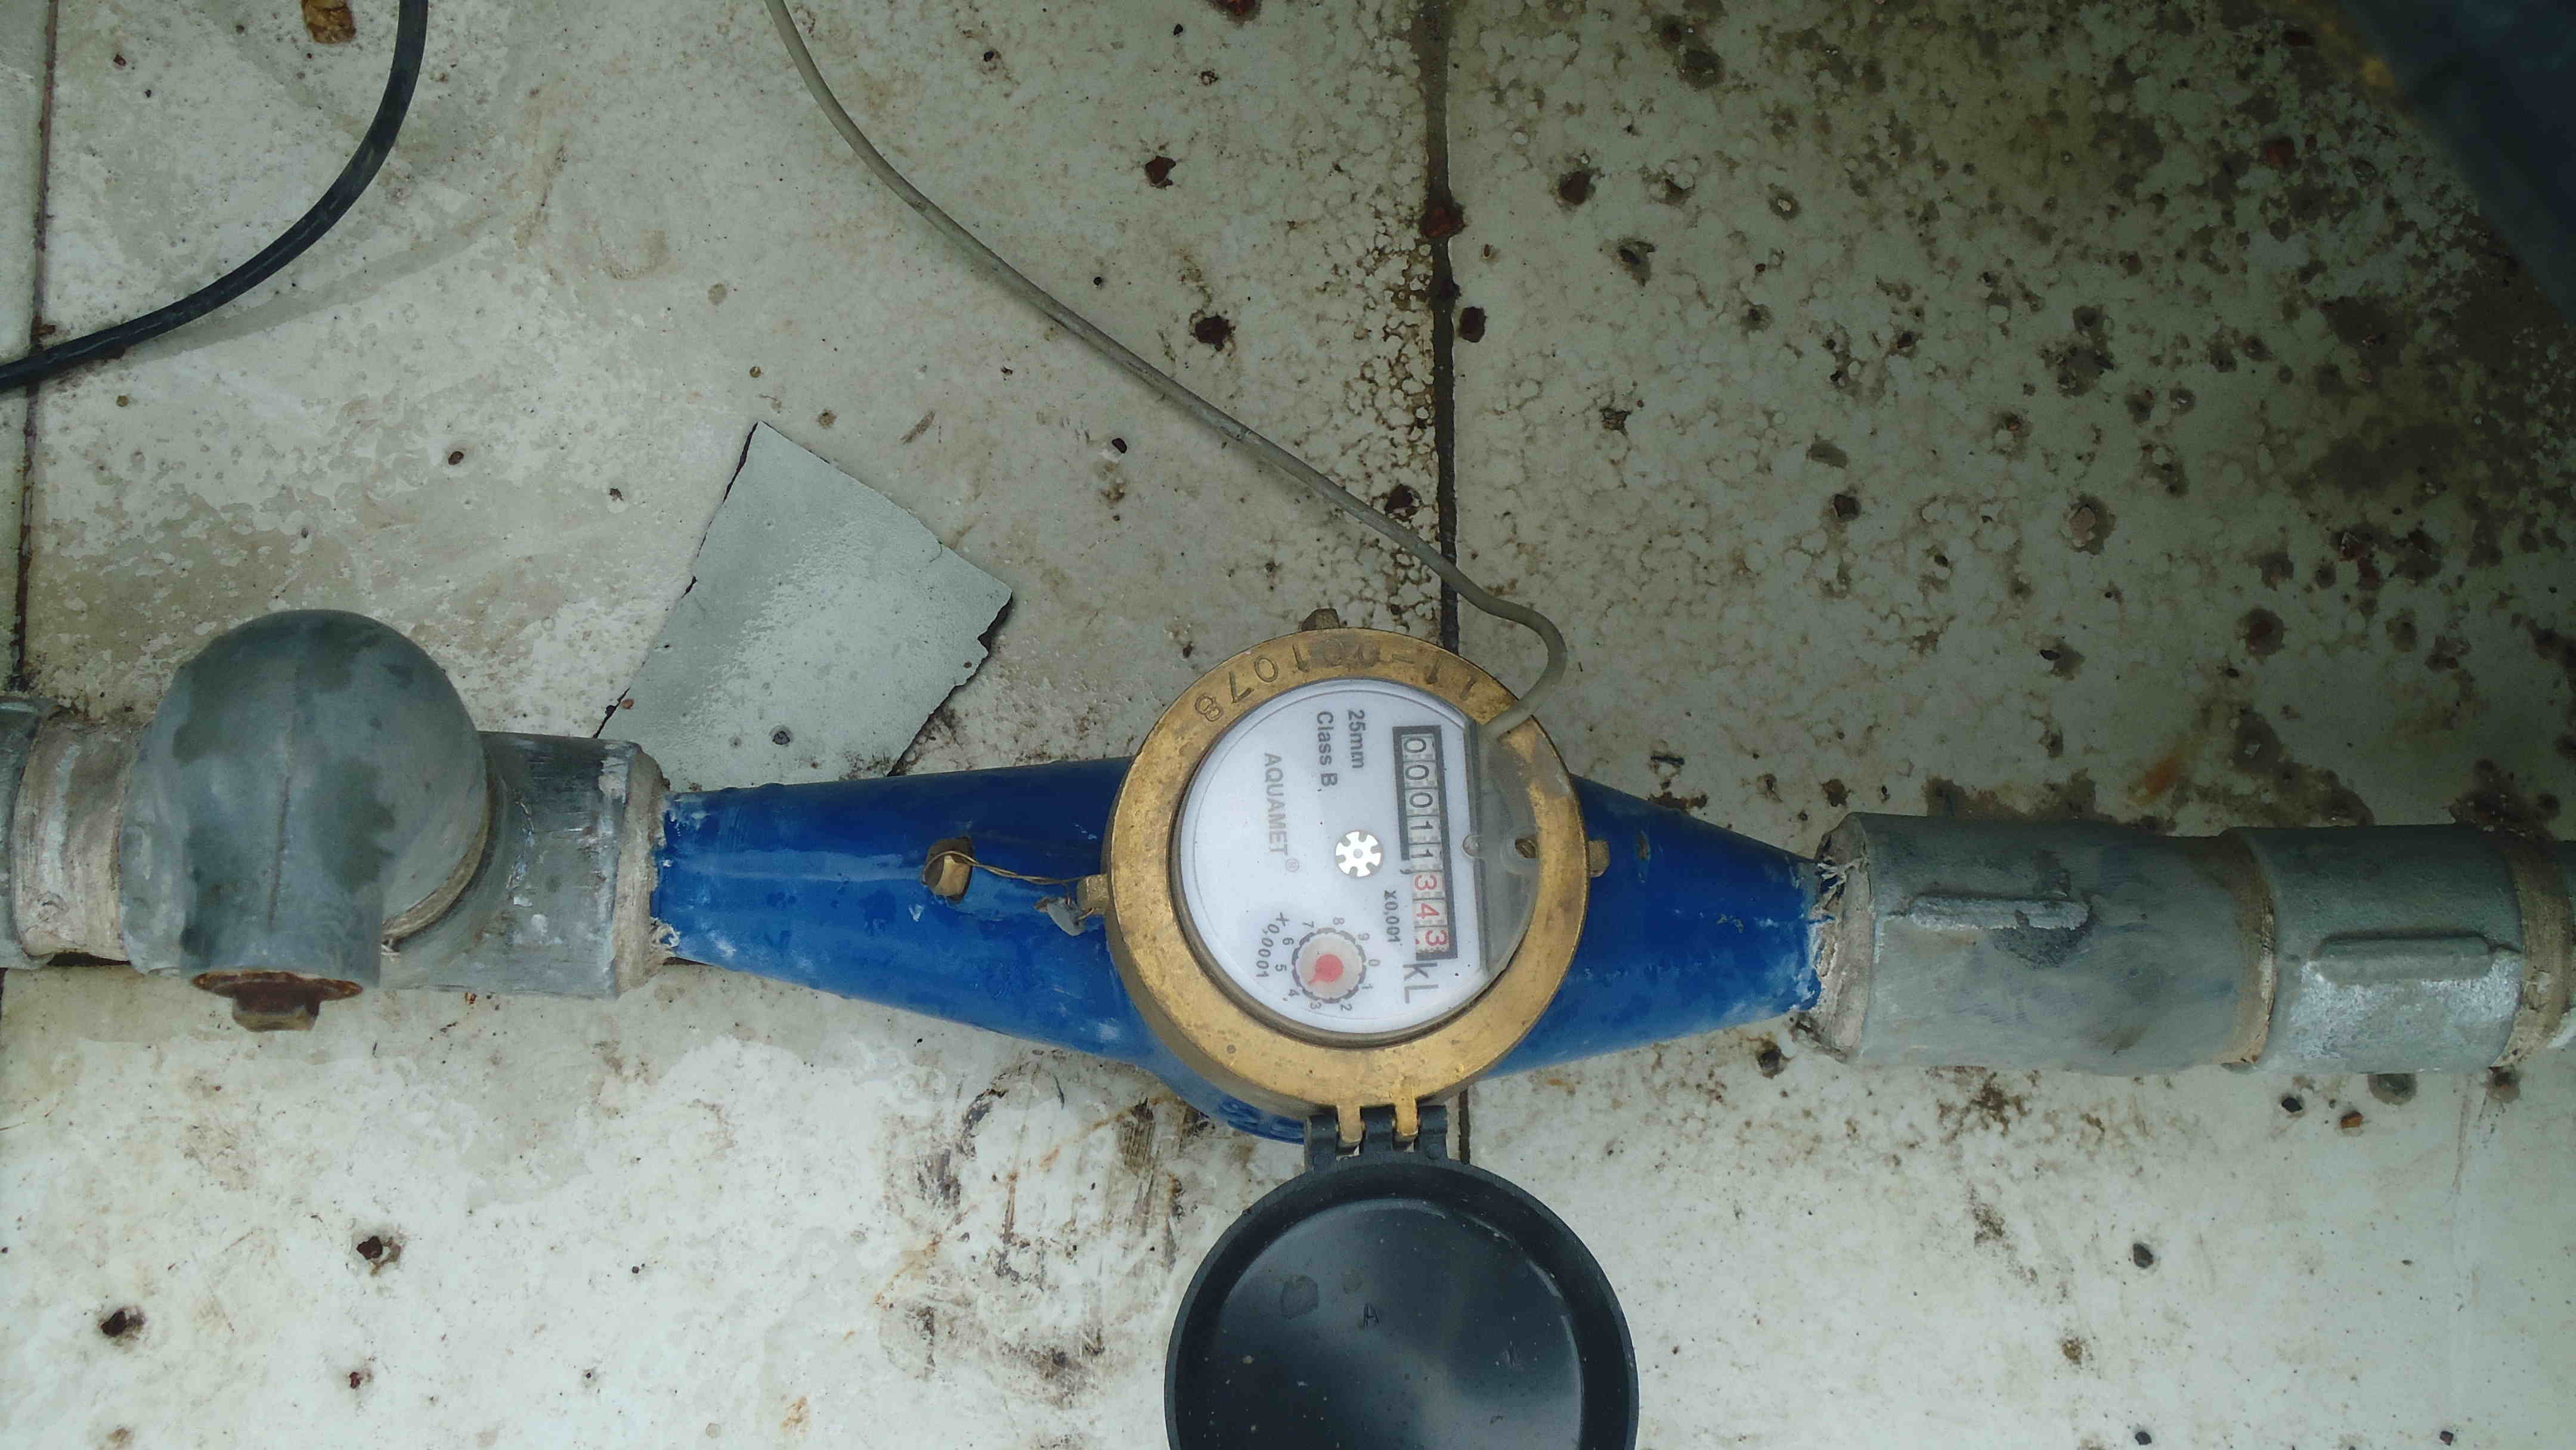
\includegraphics[scale=0.027]{./figures/water_meter.jpg}}
        \hspace{1mm}
     \subfloat[\scriptsize Android phone and Homeseer Zwave multisensor used to measure ambient parameters]{
        \label{fig:ambient}
            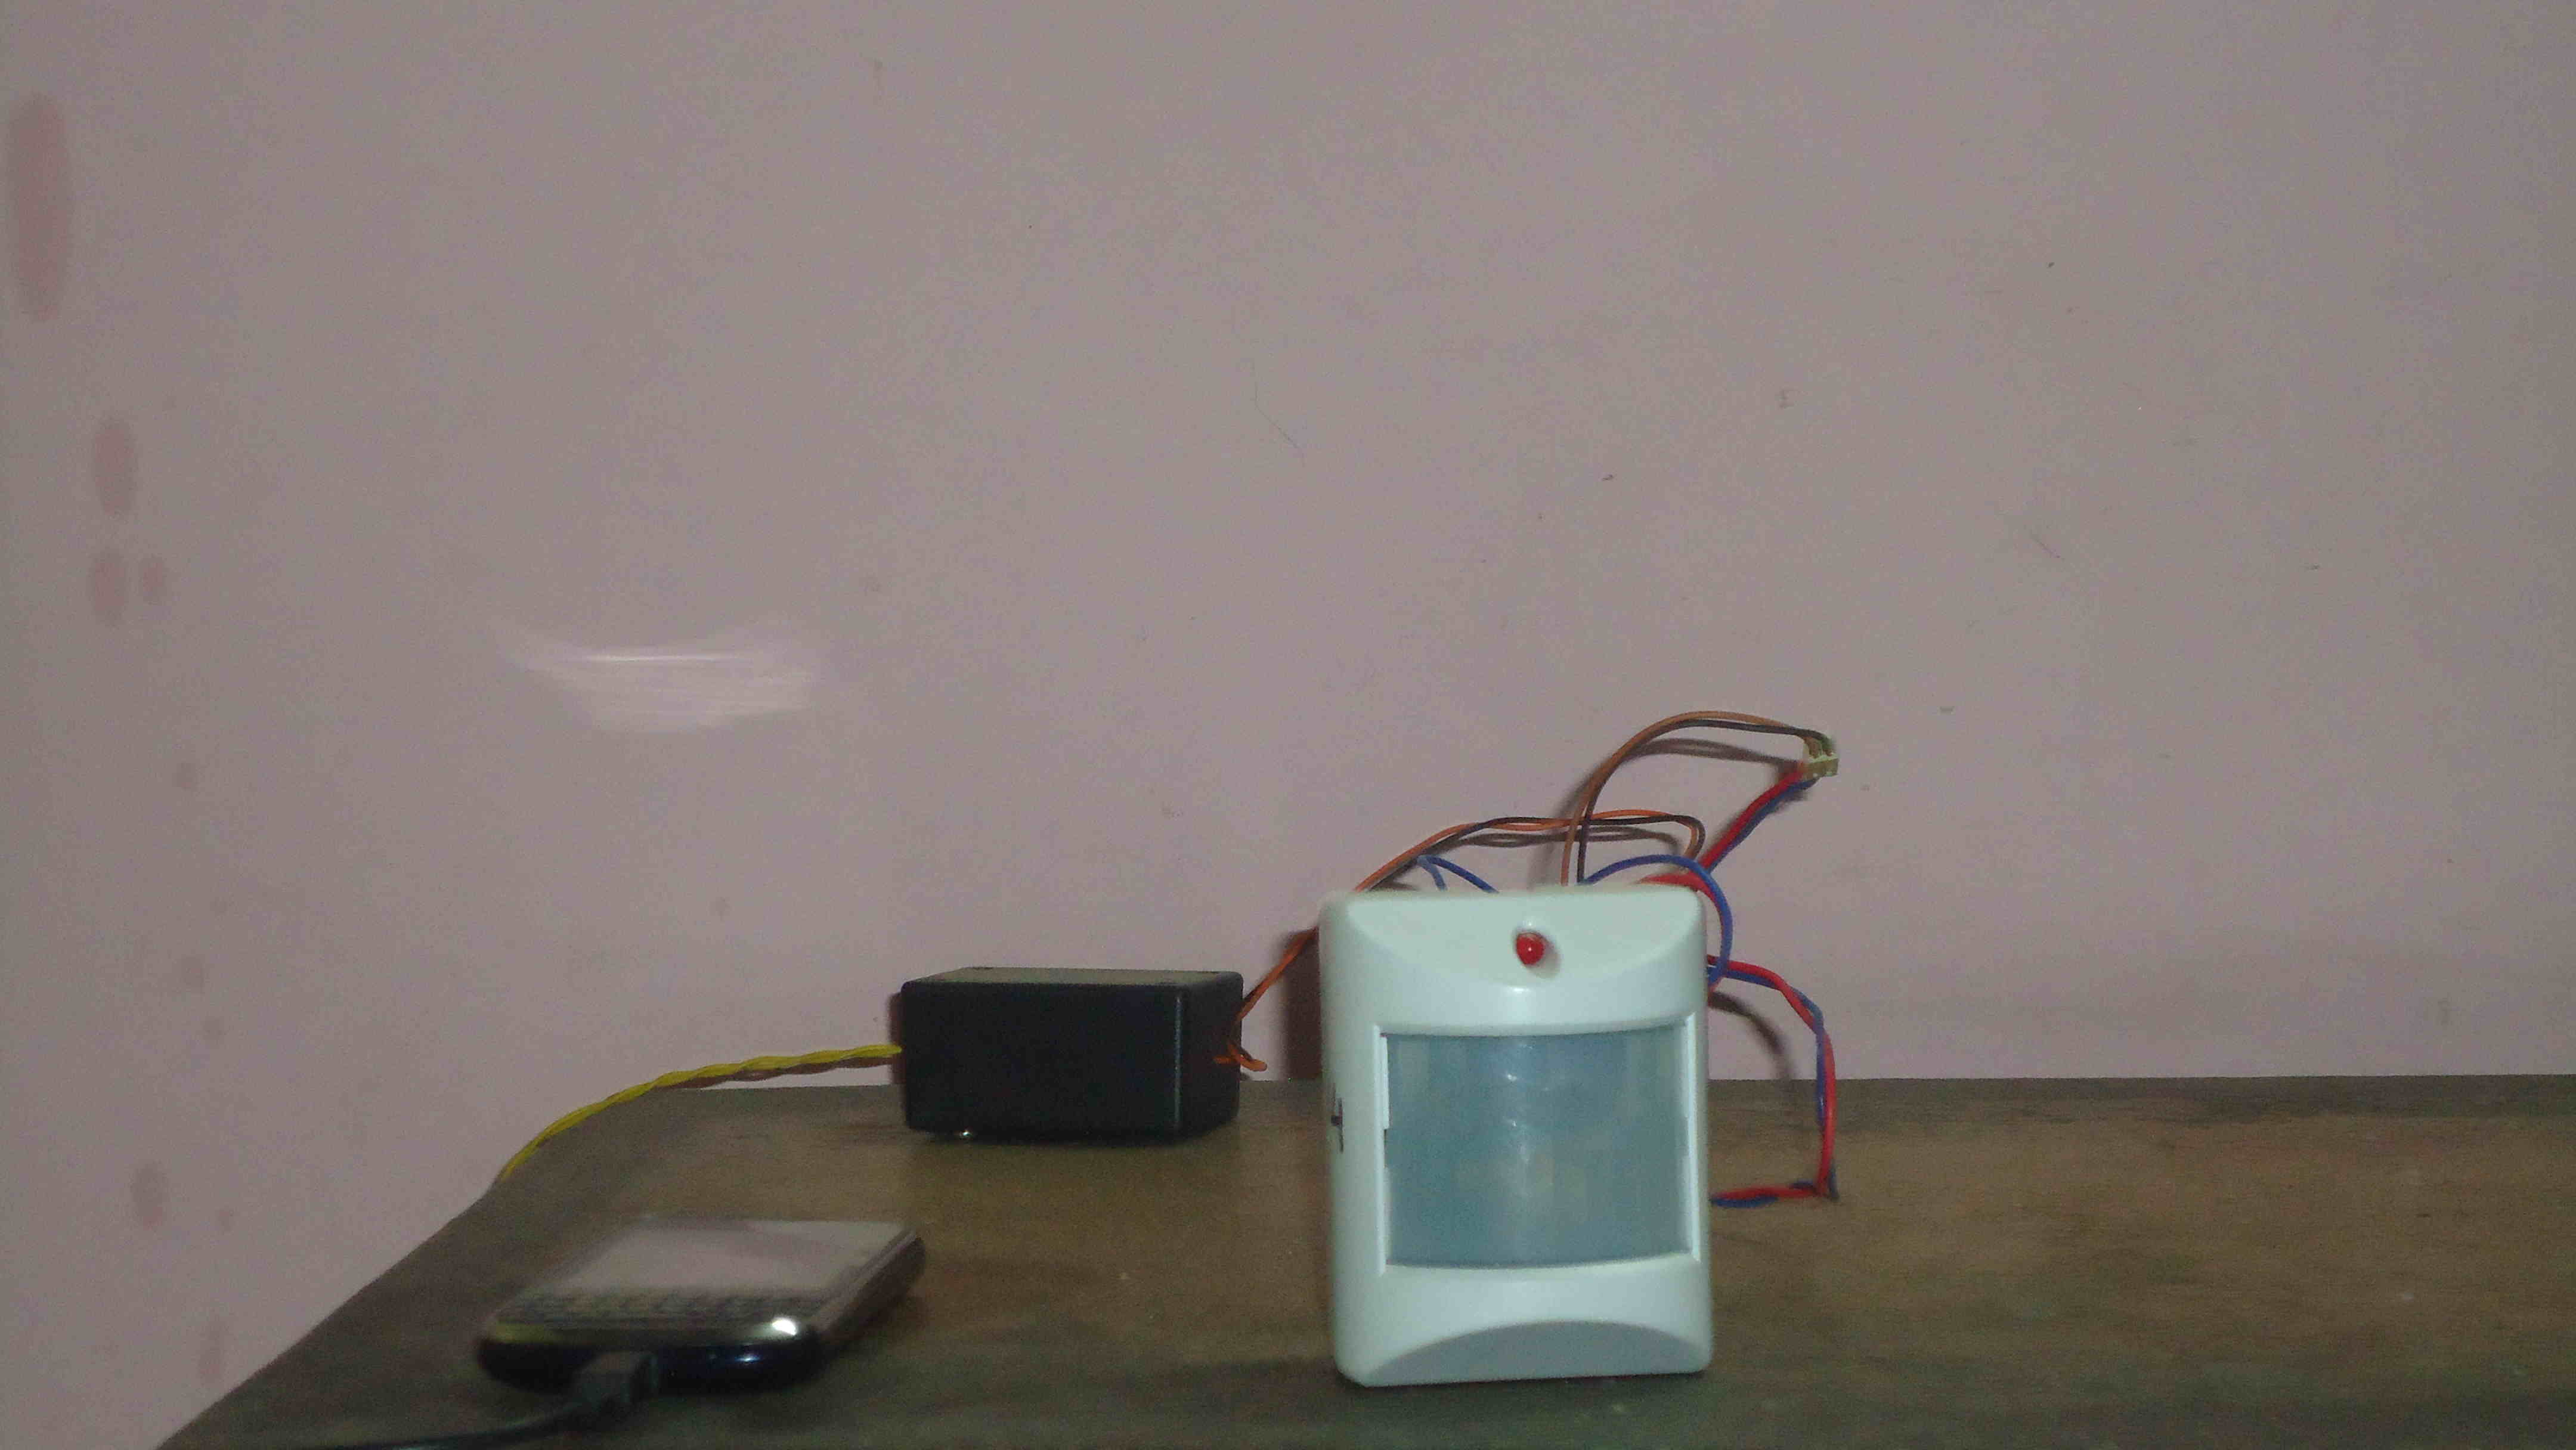
\includegraphics[scale=0.027]{./figures/ambient.jpg}}
            \hspace{1mm}
       \subfloat[\scriptsize Plug computer collecting data from ZWave controller and connected to the router via an ethernet cable]{
              \label{fig:plug}
                  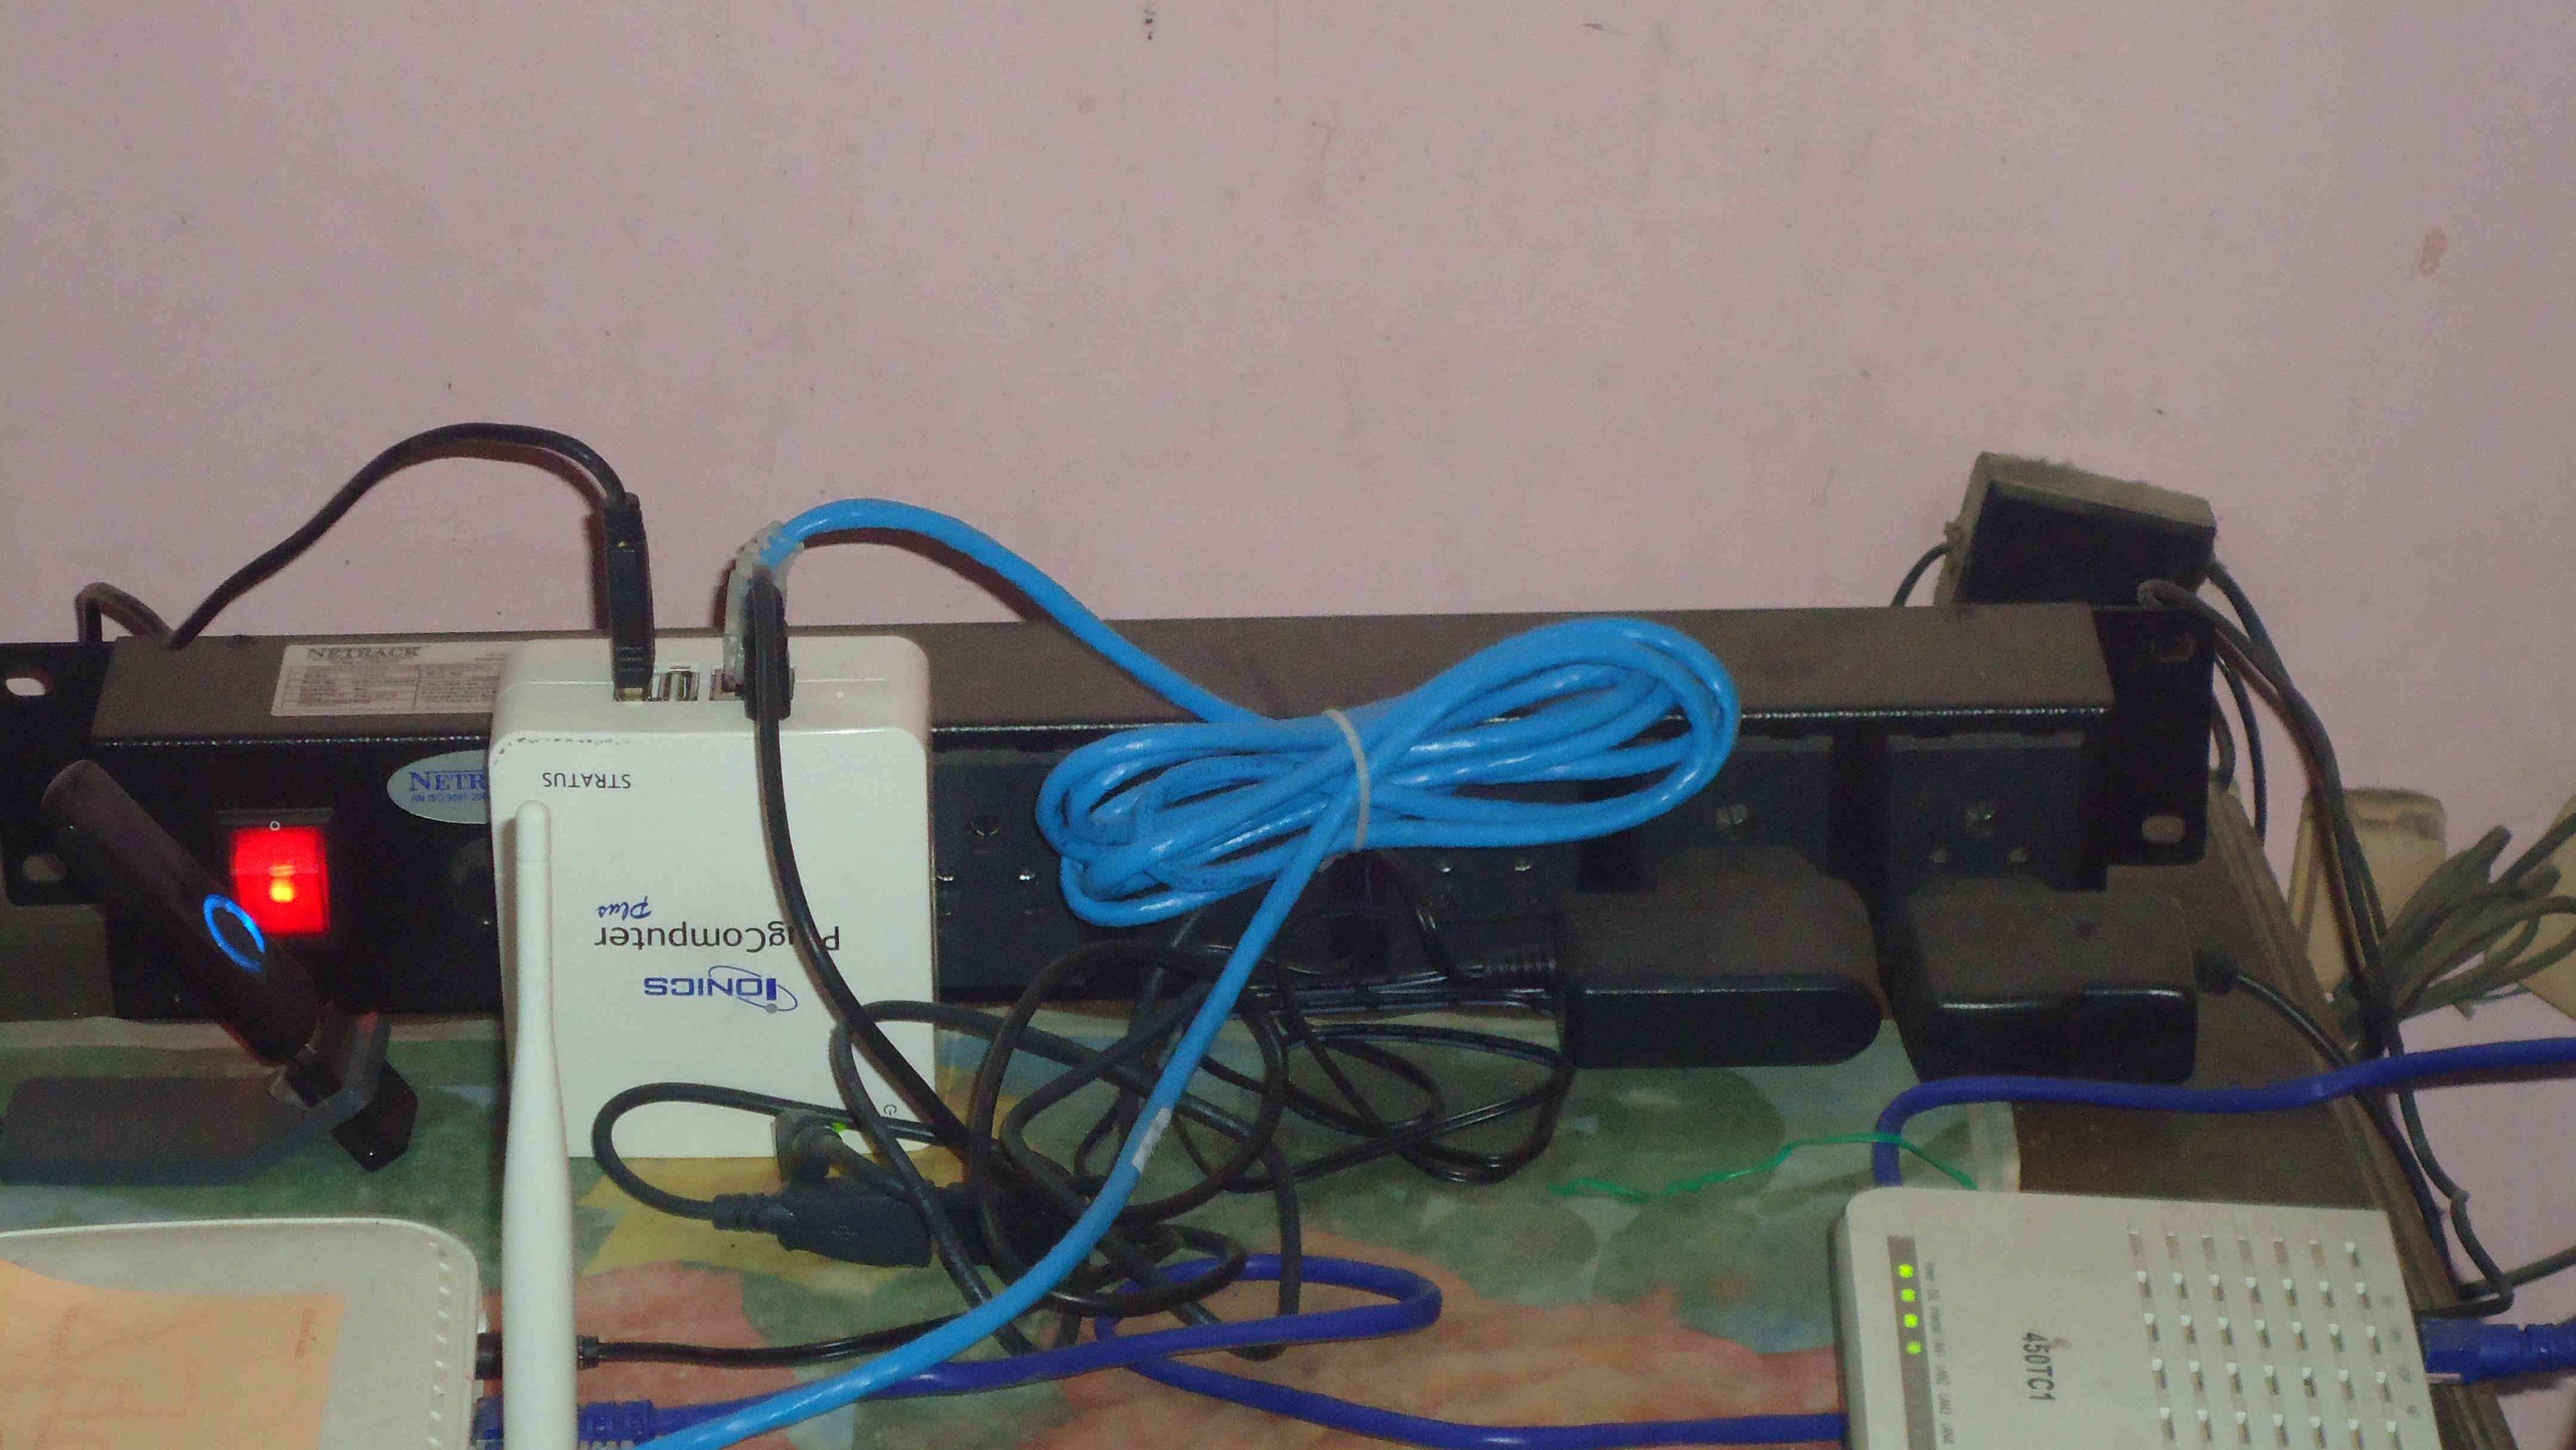
\includegraphics[scale=0.027]{./figures/plug.jpg}}
                  \hspace{1mm}
         \subfloat[\scriptsize RPi collecting water meter data using GPIO pins]{
                     \label{fig:rpi}
                         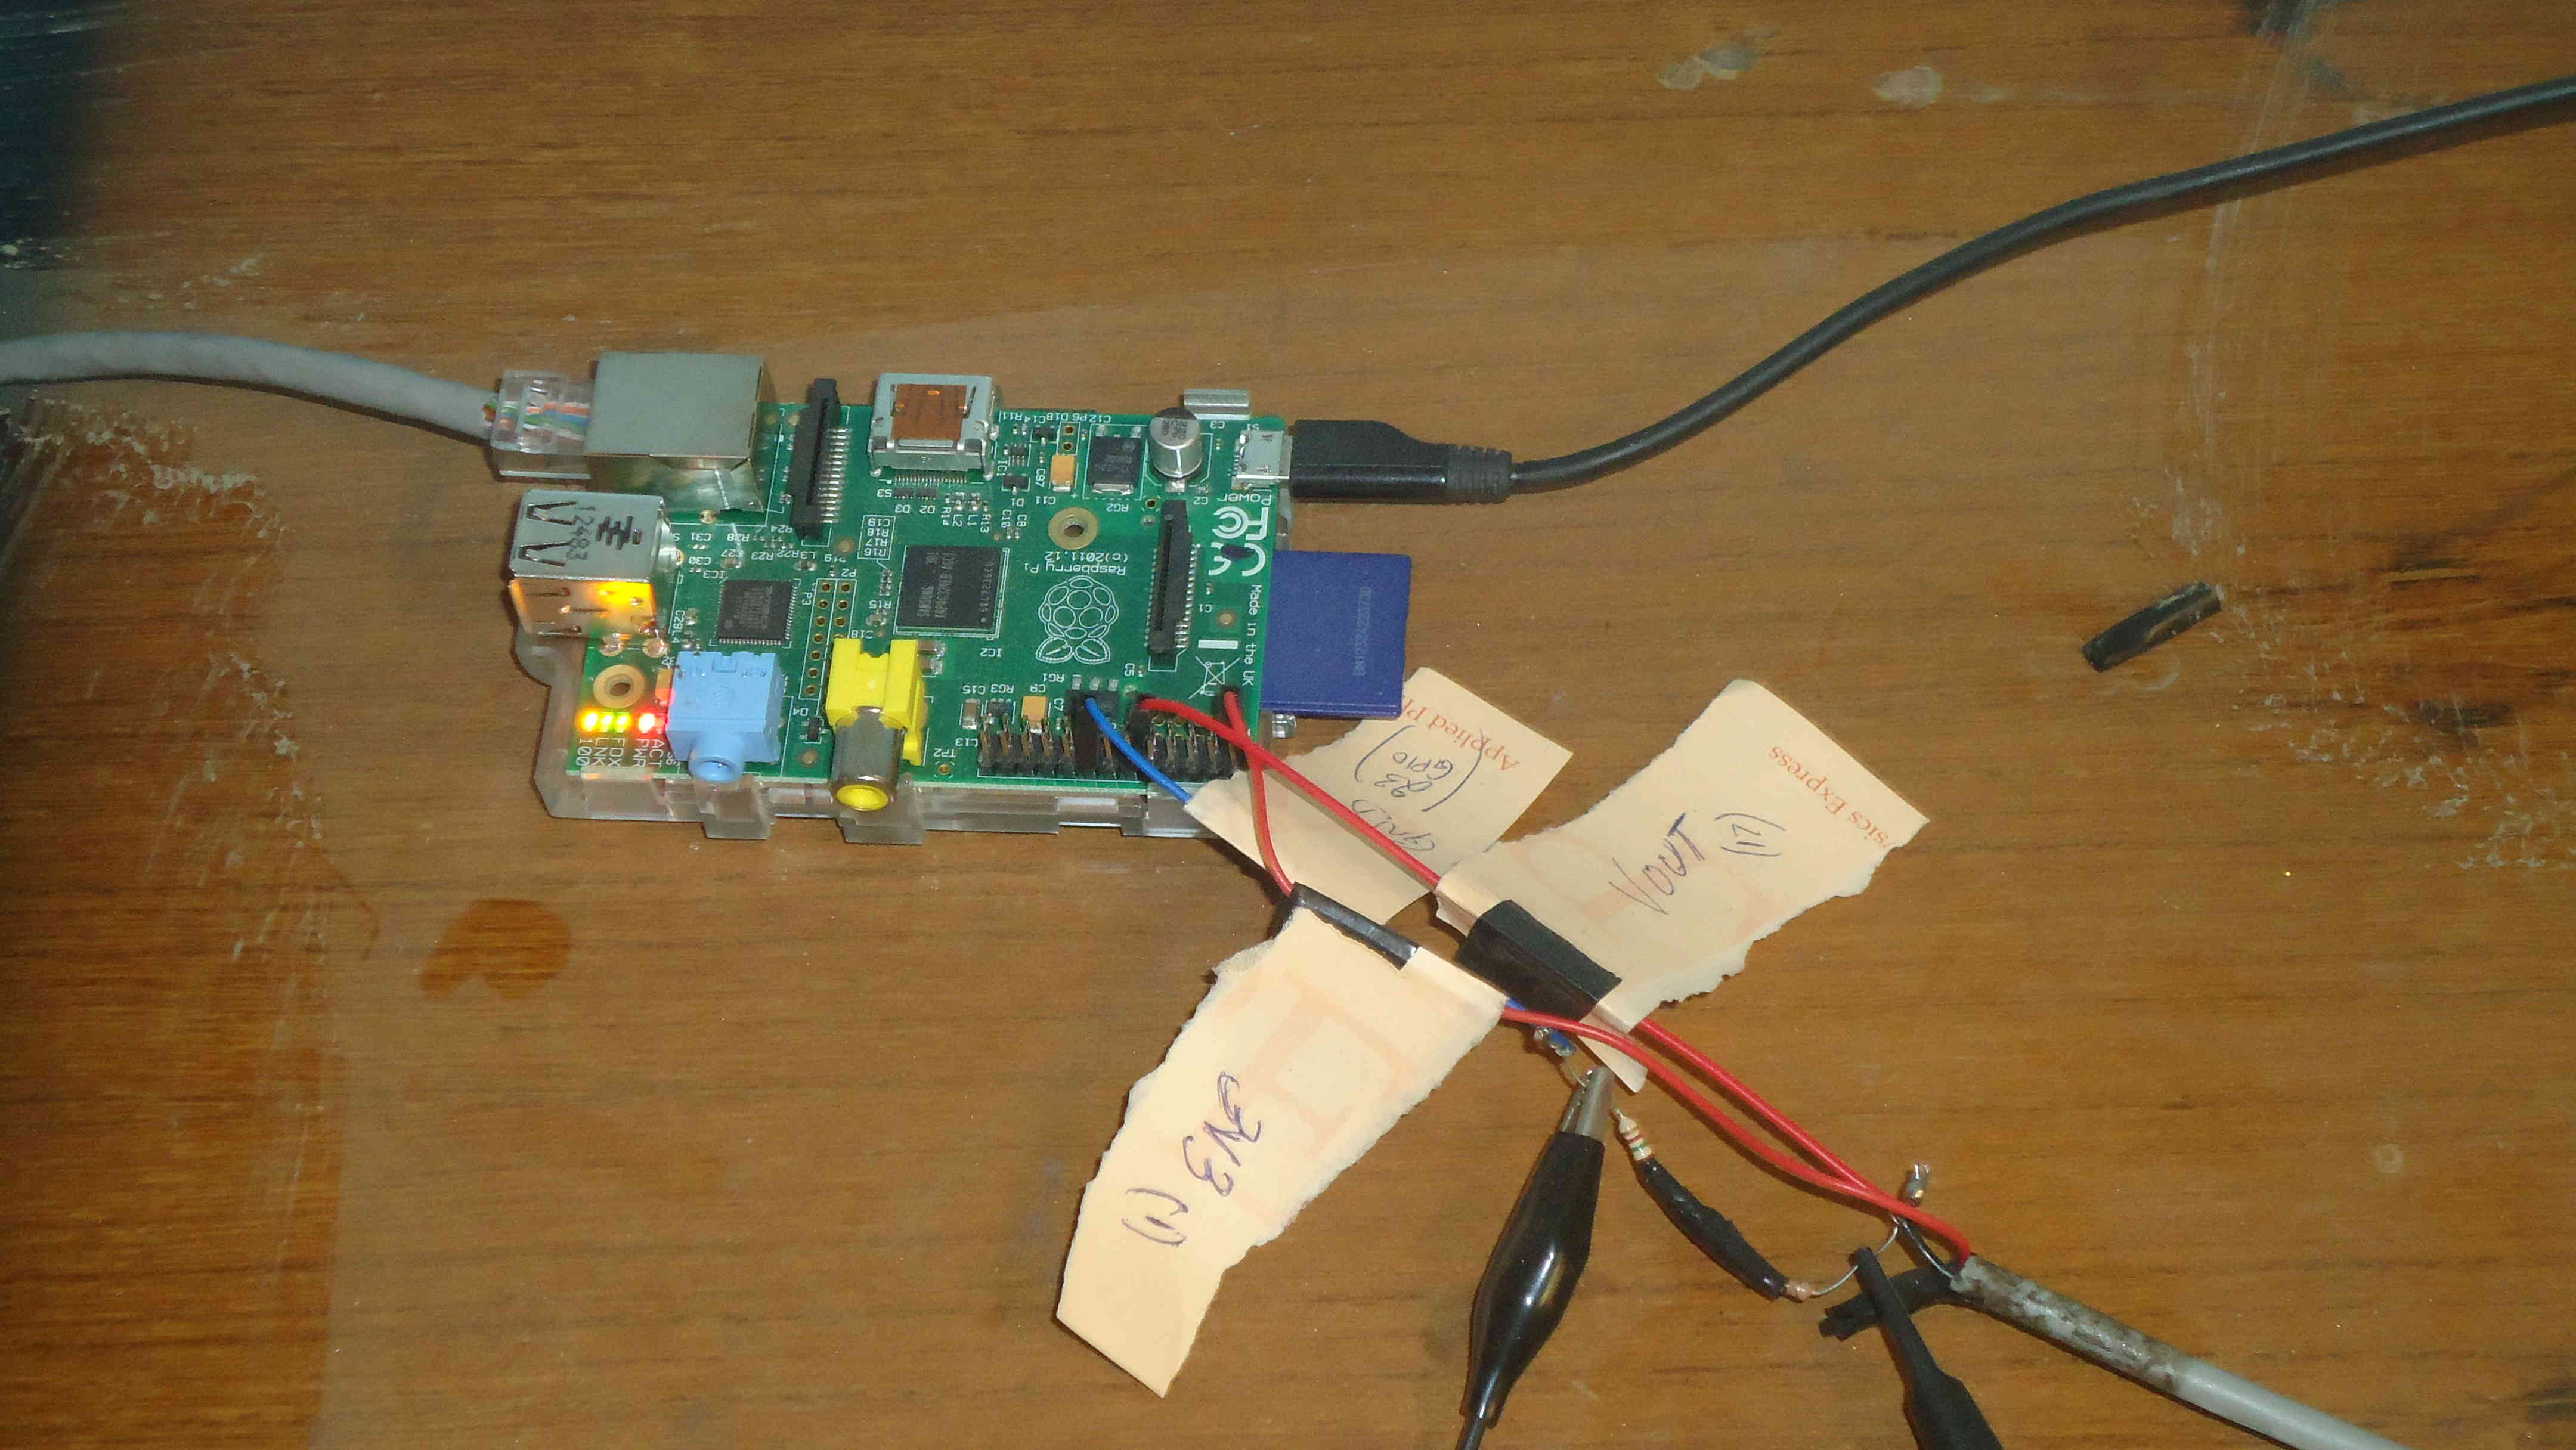
\includegraphics[scale=0.027]{./figures/rpi.jpg}}

    \caption{Sensing, computation and communication equipment used for deployment}

    \label{fig:deployment}

\end{figure*}


\section{How is this deployment different?}
\label{sec:learning}
In this section we discuss some of the key unique aspects brought forward from our deployment, which are as follows:

\begin{figure*}[t!] 
    
    \subfloat[\scriptsize Power outage vs Time]{
    \label{fig:failure_time}
    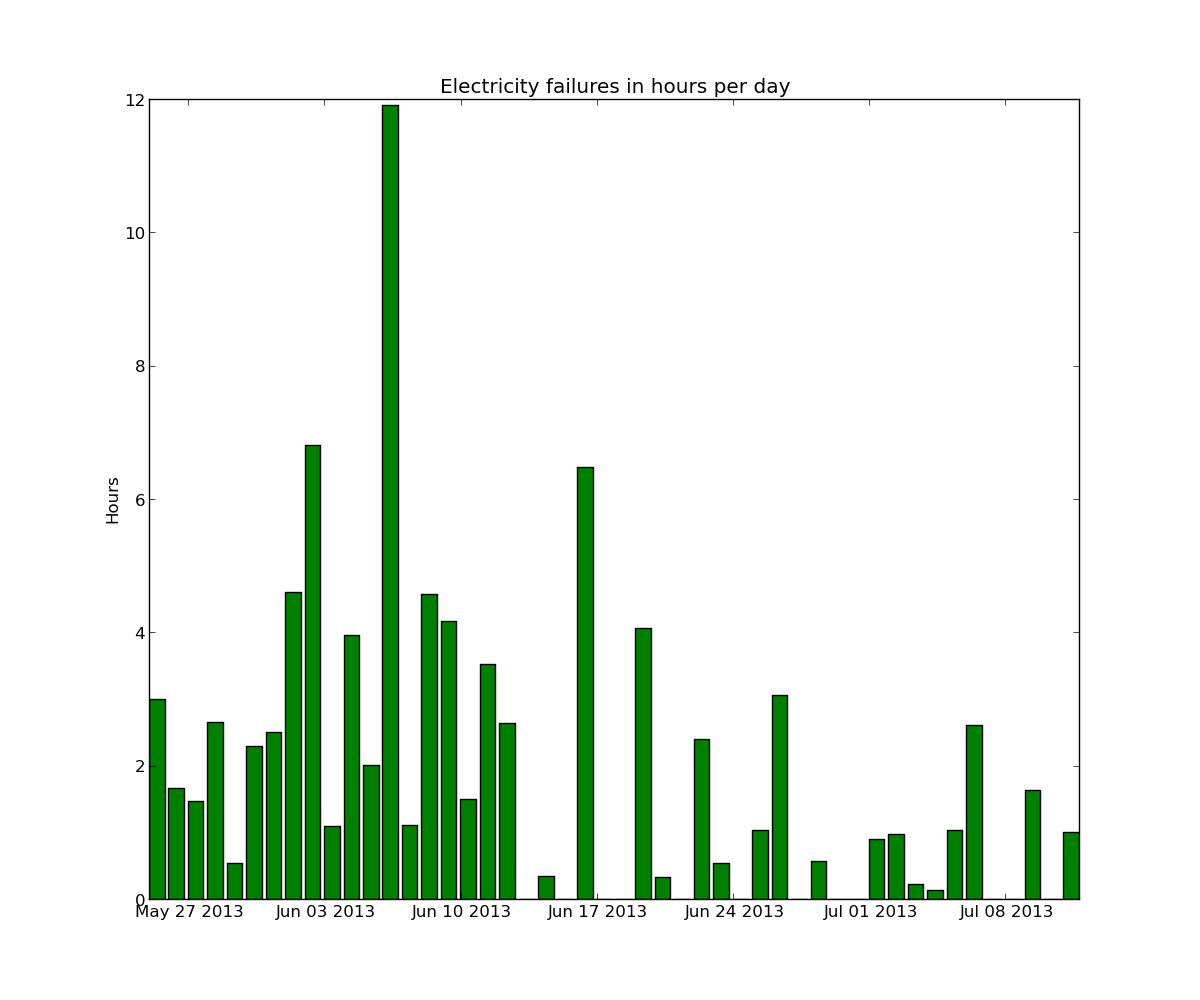
\includegraphics[scale=0.15]{./figures/electricity.png}}
    \hspace{1mm}
     \subfloat[\scriptsize Power outage durations ]{
        \label{fig:failure_duration}
        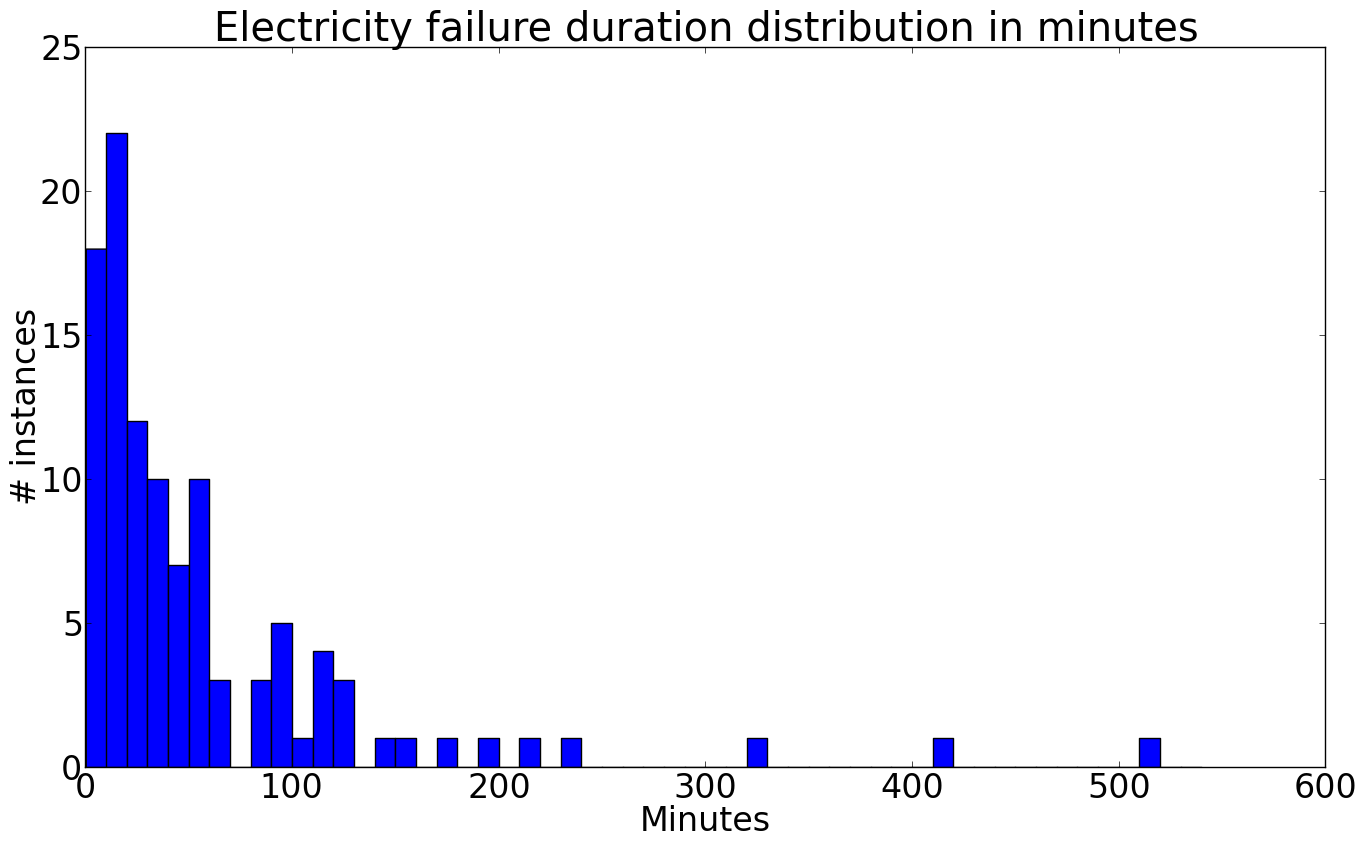
\includegraphics[scale=0.15]{./figures/failure_durations.png}}
       \hspace{1mm}
     \subfloat[\scriptsize Power outage by hour of day]{
             \label{fig:failure_hour}
             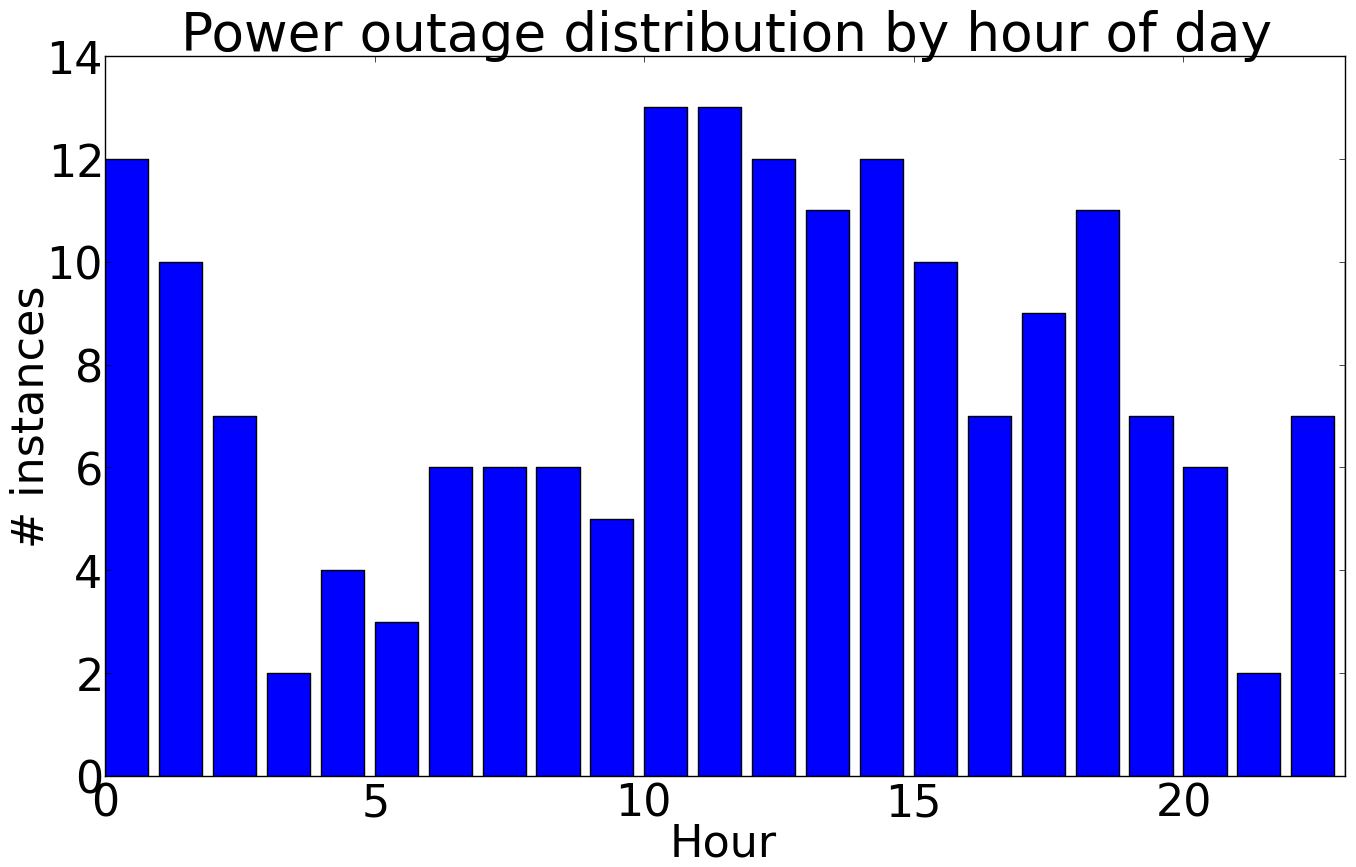
\includegraphics[scale=0.15]{./figures/outage_by_hour.png}}
              \vspace{-4mm}
             \newline
            
          \subfloat[\scriptsize Voltage fluctuations in a typical day. Rated voltage is 230 V]{
                  \label{fig:voltage}
                  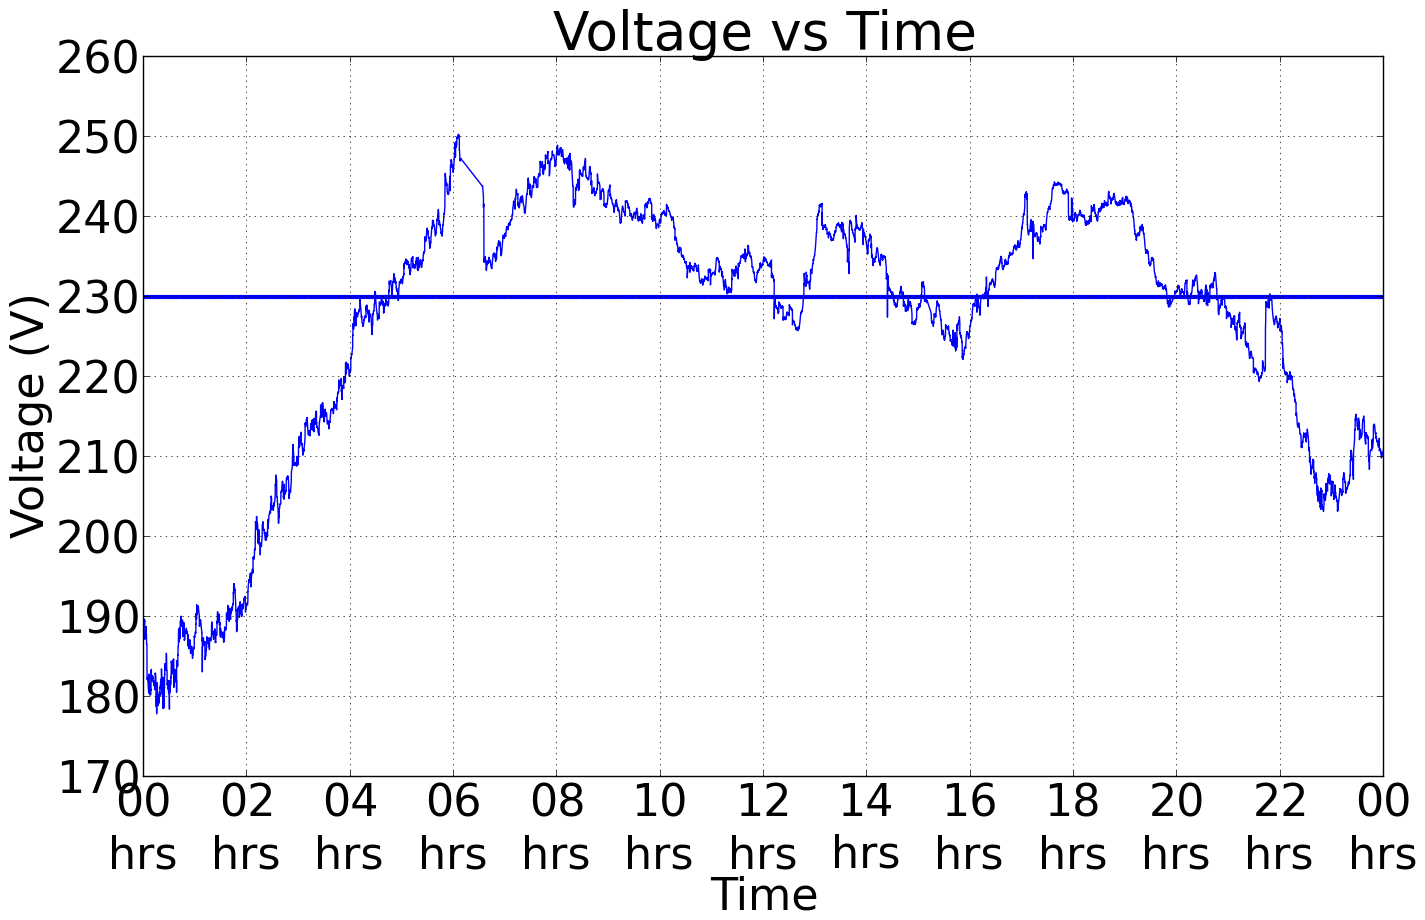
\includegraphics[scale=0.15]{./figures/voltage.png}}
          \subfloat[\scriptsize Frequency fluctuations in a typical day. Rated frequency is 50 Hz]{
                            \label{fig:frequency}
                            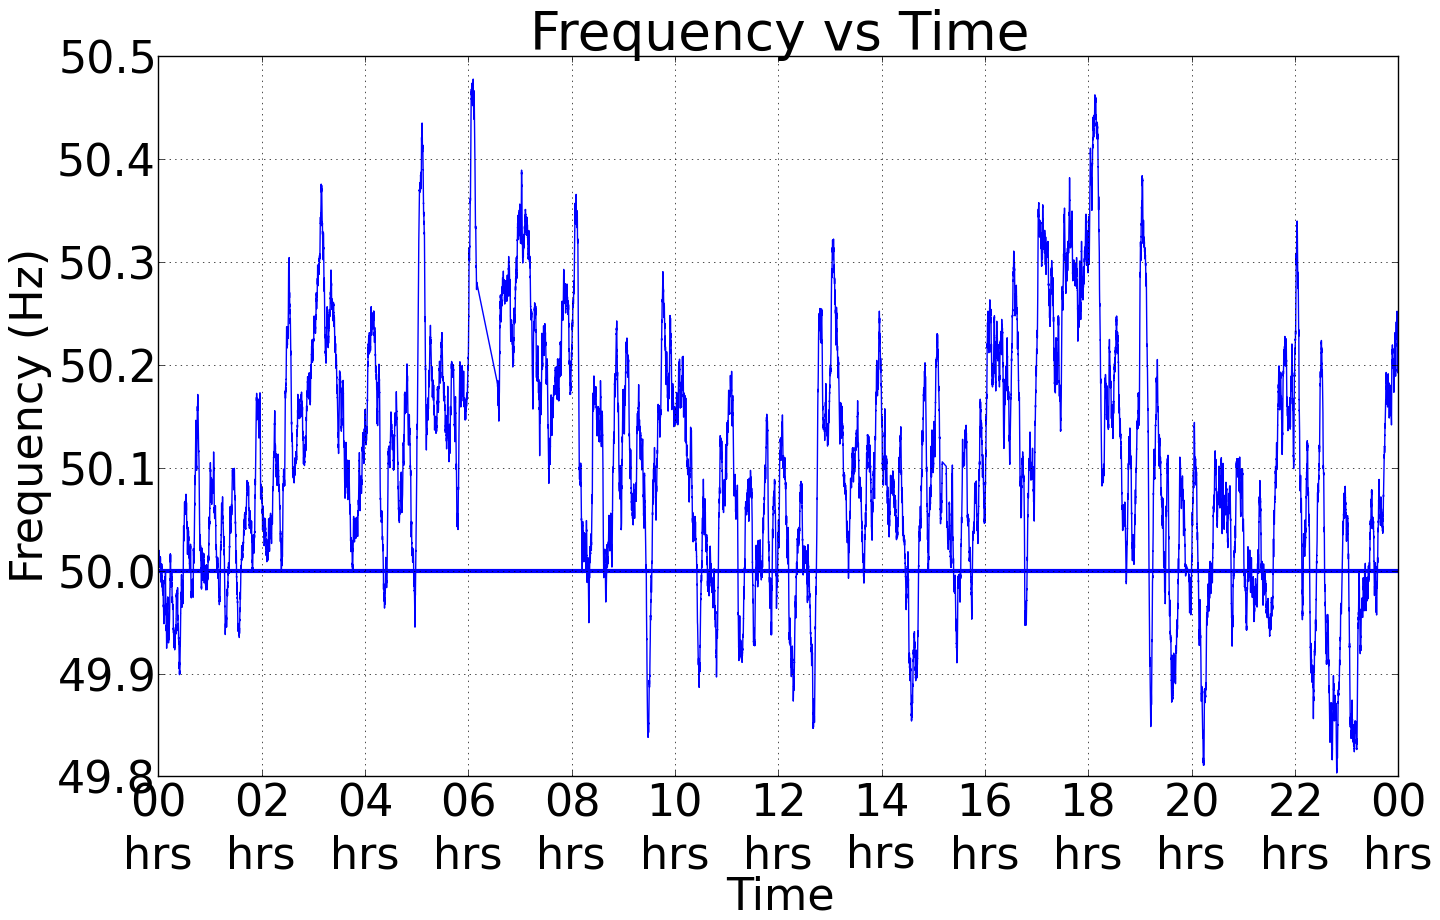
\includegraphics[scale=0.15]{./figures/frequency.png}}
          \subfloat[\scriptsize Observed voltage just before power outage during night hours (10 PM to 1 AM). Rated voltage is 230 V]{
                            \label{fig:voltage_before_outage}
                            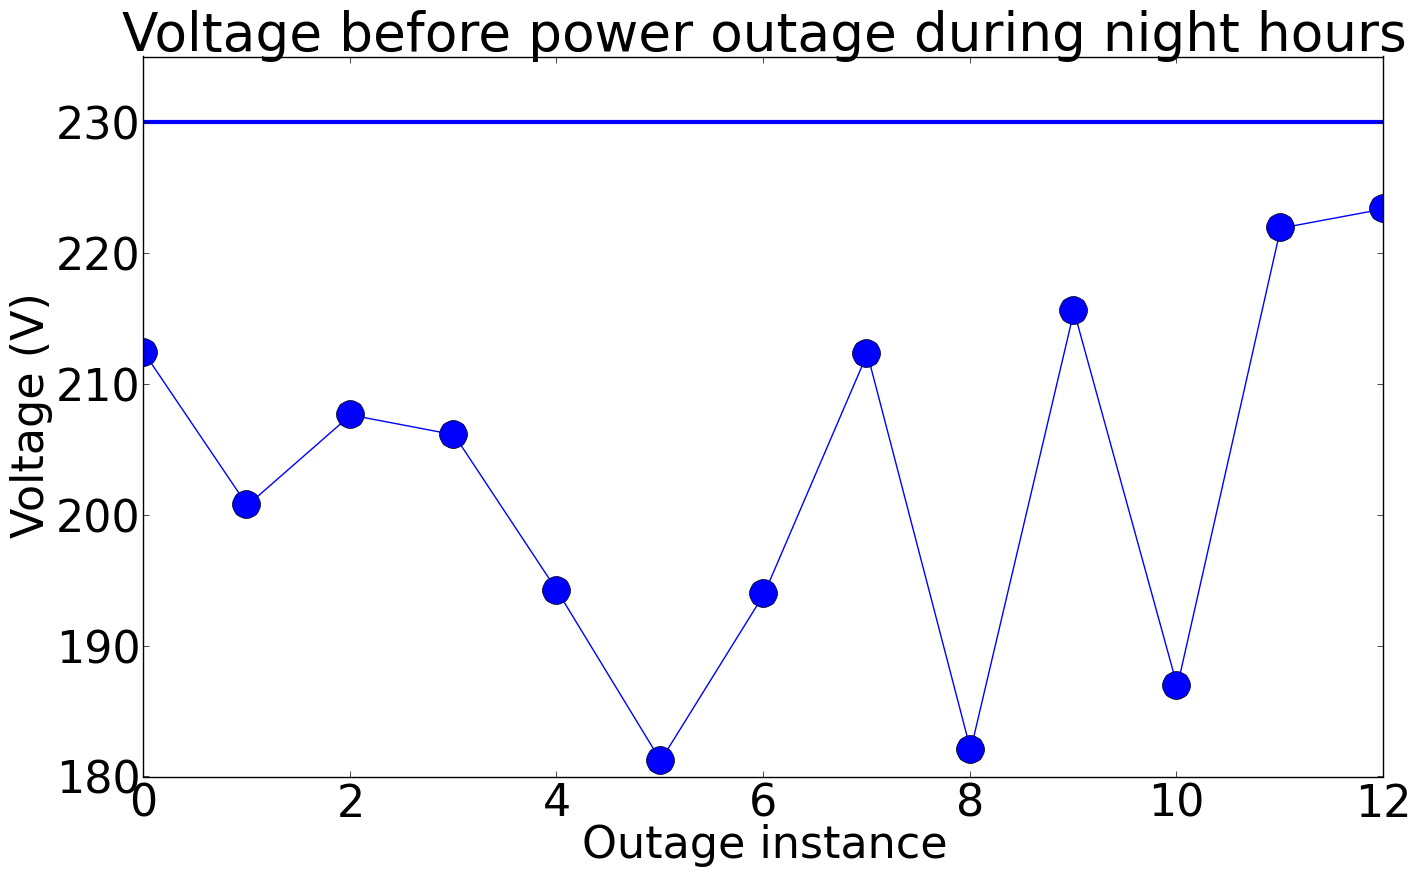
\includegraphics[scale=0.15]{./figures/voltage_before_outage.png}}
   
    \caption{Unreliable grid}

    \label{fig:unreliable}

\end{figure*}
\noindent \textbf{Unreliable grid is commonplace:} Load shedding or rolling blackout are common in developing countries, owing to several reasons such as improper infrastructure management, high demand and low electricity production. In India, power outages are common in summers when load is high due to usage of air conditioners. As a result, voltage fluctuations or brownouts are also common.

\noindent We collected various statistics from our deployment which illustrate these aspects. \figref{fig:failure_duration} shows power outages in number of hours per day during June-July 2013. Power outage for upto 12 hours has been reported on some days. \figref{fig:failure_duration} shows the duration in minutes of power outages. A total of 107 power outages were reported in the 61 day period. While the average power outage lasted about 1 hour, there were outages lasting upto 9 hours. \figref{fig:failure_hour} shows the power outage distribution by hour of the day. It can be seen that there are maximum outages around 10 AM in the morning and around midnight. These times correspond to office time and night time when air conditioners in most homes are on and there is heavy load on the grid. \figref{fig:voltage} shows the voltage fluctuations in a typical day, where it can be seen that voltage is fluctuating from 180 to 250 Volts. We can observe that voltage drops during peak load hours. \figref{fig:voltage_before_outage} shows that voltage just before power outage in night hours (10 PM to 1 AM), when load is expected to be maximum. We can observe that voltage is well below rated voltage of 230 V. This is in coherence with previous work~\cite{nplug}, which hypothesized that frequency and voltage indicate load on the grid. \figref{fig:frequency} shows fluctuation in frequency in a typical day.

\noindent Due to unreliable nature of grid, we ensured that all our systems were capable of automatically starting after a power outage. We put our scripts for data collection and upload in Linux startup script. This provided us another advantage. If we observed that a system was down, we could just ask the home occupant to repower the system. This ensured that there was minimal data loss till the time our researchers could visit the site and repair the fault.

\begin{figure}
\subfloat[\scriptsize \% internet packet drop vs time]{
    \label{fig:network}
    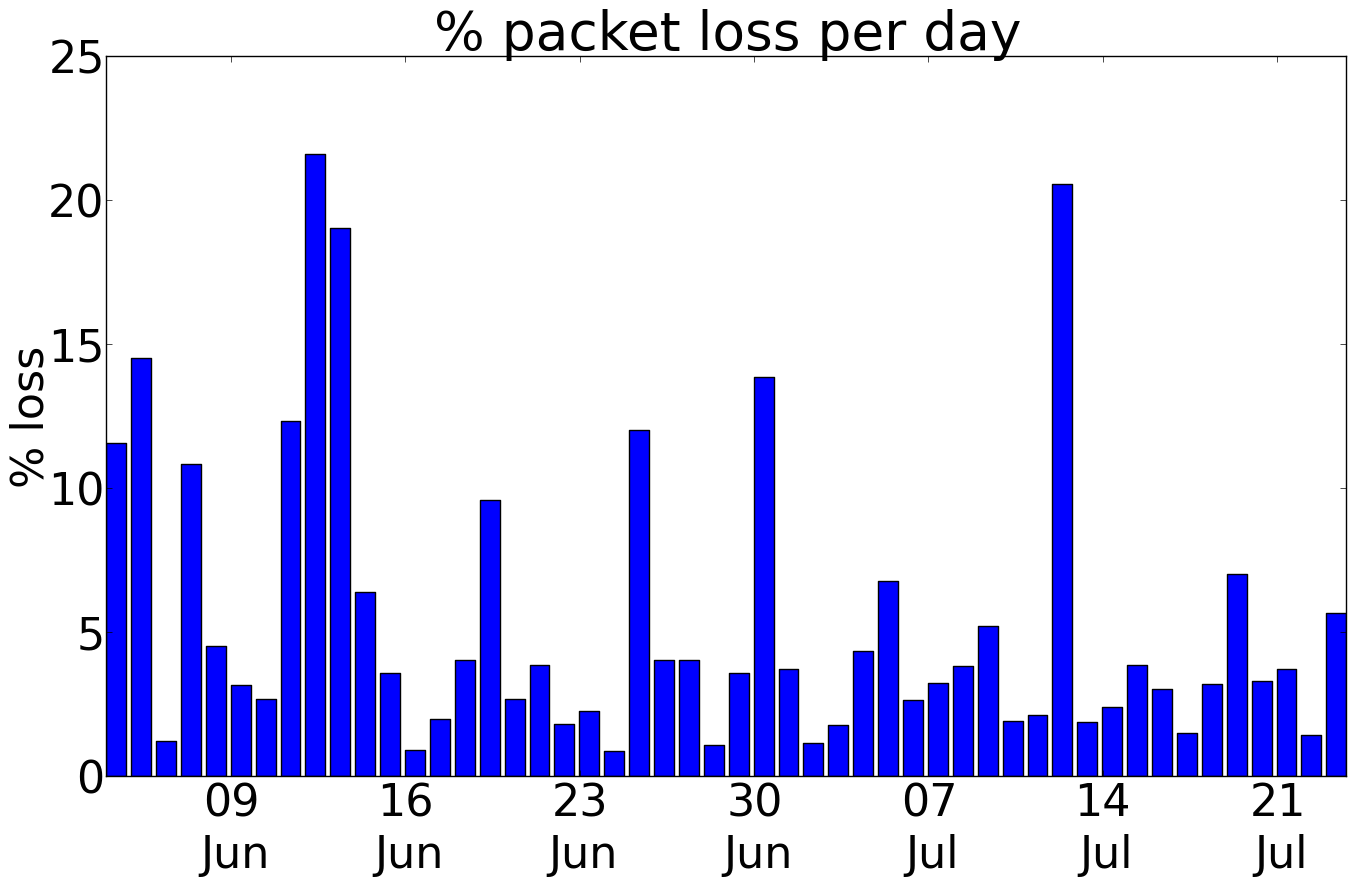
\includegraphics[scale=0.115]{./figures/network.png}}
        \subfloat[\scriptsize \% internet packet drop distribution]{
        \label{fig:network_hist}
        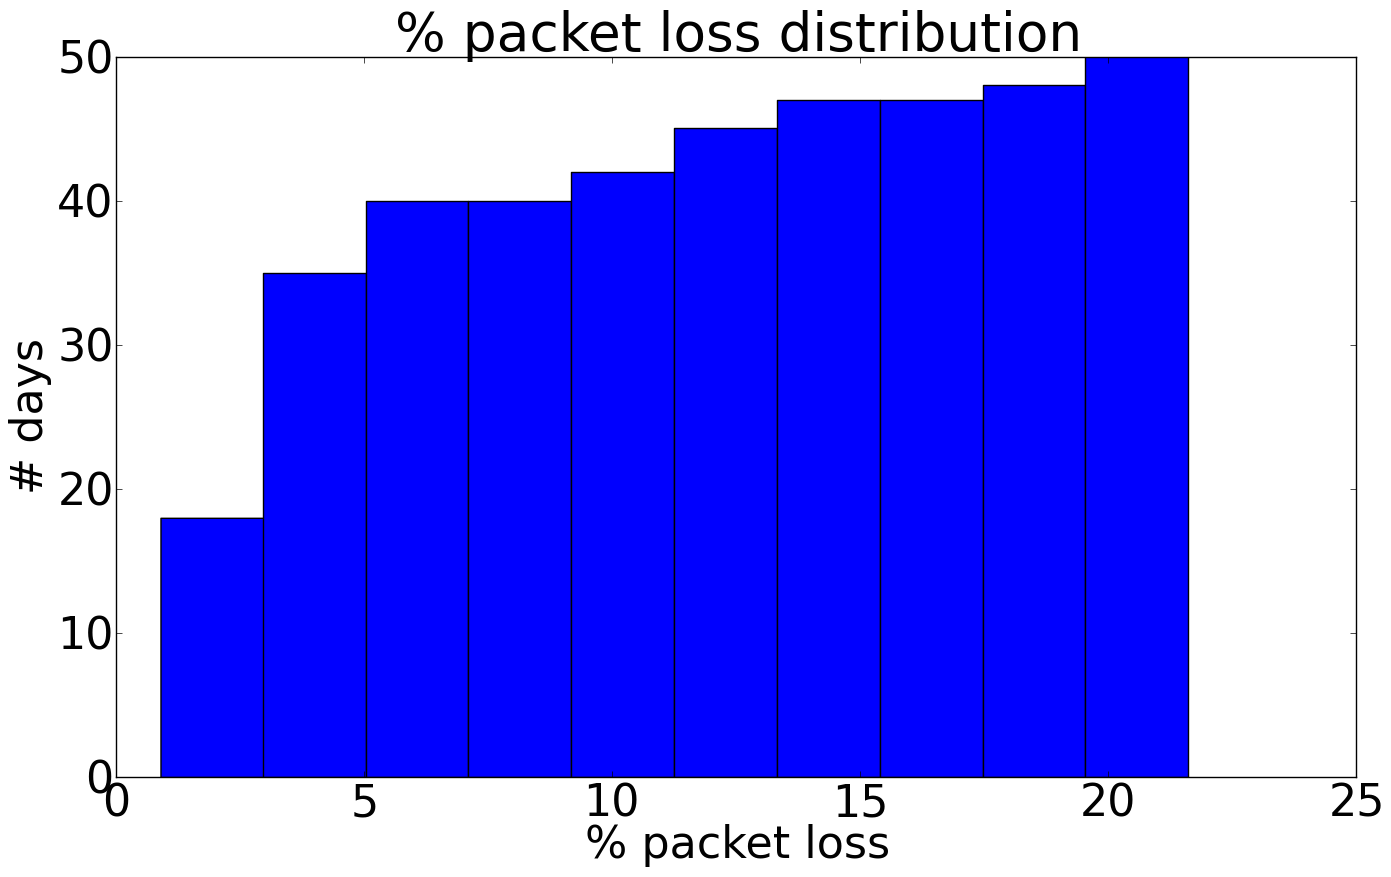
\includegraphics[scale=0.115]{./figures/network_hist.png}}
  \caption{Unreliable internet}
  
      \label{fig:unreliable_internet}
\end{figure}

\noindent \textbf{Unreliable internet connectivity:} While India has one of the fastest growing internet population, only 11\% of the total population is connected to internet, the corresponding figure in USA is 78\%~\cite{meyer}. Average connection speed in India is 1.3 Mbps, the corresponding numbers in developed countries are in excess of 10 Mbps~\cite{state_of_internet}. Even though the condition of internet has vastly improved in the previous few years, from practical experience, we have found it to unreliable. We found internet would be unavailable several times during the day and sometimes it would be too slow. This was a prime motivation behind local storage and periodic data upload, which we have proposed in \paradigm. Using \paradigms all the data eventually gets synced up to the main server and from there to the cloud over the internet. We, thus, believe that for deployments where internet is unreliable, architectures such as \paradigms should be adopted.

\noindent To illustrate the need for \paradigms, we collected network statistics from our deployments. We sent a packet consisting of 15 internet ping requests every 15 seconds and reported packet drop. \figref{fig:network} shows that packet drop of upto 25\% was observed on certain days. The average packet drop was around 6\% per day. \figref{fig:network_hist} shows a histogram plot of \% packet drop. It can be seen that on 1/6 fraction of total days, \% packet loss is greater than 10\%.


\begin{figure}
\subfloat[\scriptsize Before repair]{
    \label{fig:before_repair}
    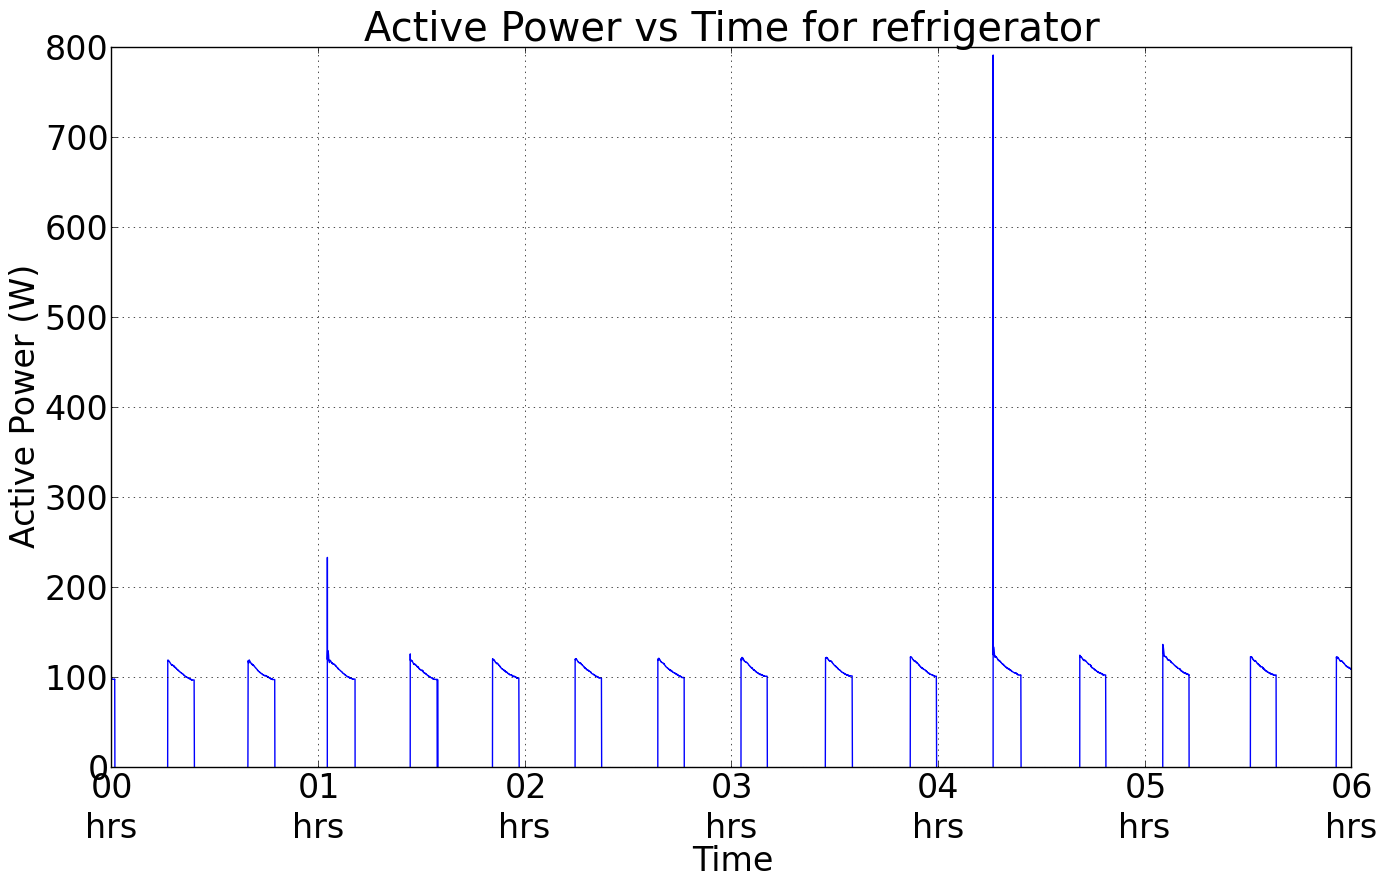
\includegraphics[scale=0.12]{./figures/before_repair.png}}
     \subfloat[\scriptsize After repair ]{
        \label{fig:after_repair}
        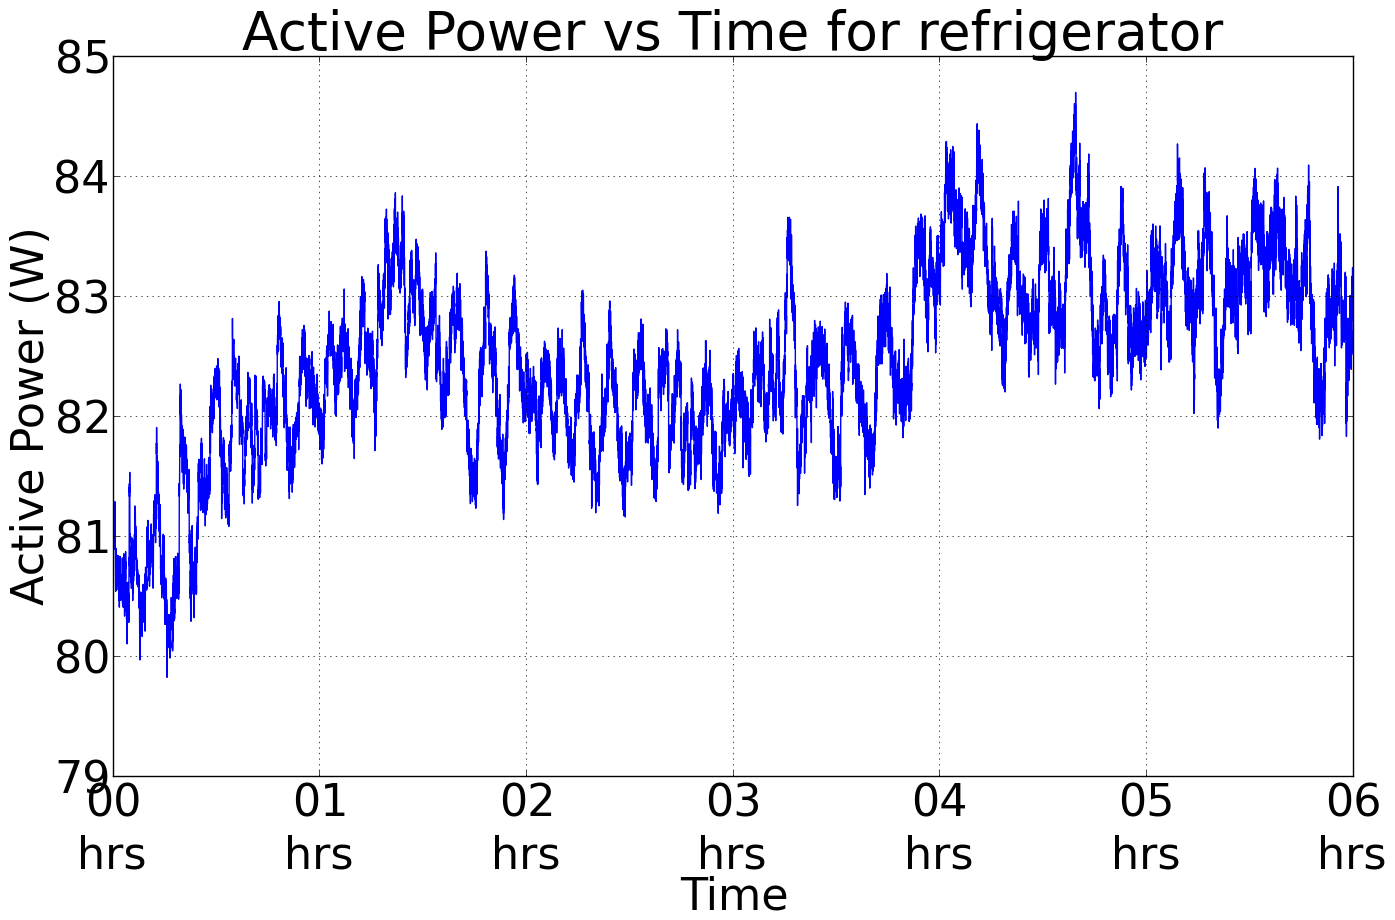
\includegraphics[scale=0.12]{./figures/after_repair.png}}
       
   
    \caption{Refrigerator power consumption}

    \label{fig:metadata}

\end{figure}
	
\noindent \textbf{Importance of meta data collection:} We collected metadata associated with electrical appliances throughout our deployment. We collected parameters such as appliance name, age, mode of usage (for instance air conditioner set temperature). We believe this detailed metadata can enhance NILM and can provide useful insights for conserving electricity. For instance, the home refrigerator was sent for repairing on 2$^{nd}$ July. \figref{fig:before_repair} and \figref{fig:after_repair} show the active power consumption before and after repair. We found that after repair the refrigerator was configured in coolest mode (lowest temperature), while before repairing, it was configured in least coolest mode (highest temperature). After repair the refrigerator was found to be consuming 1KWh more per day (which is 140\% above normal). Moreover, its duty cycle pattern was modified significantly. This metadata can be useful to NILM approaches which model appliance usage duration as one of their parameters.

\noindent \textbf{Load specifics:} Electrical load setting in India are different from that in the USA and Europe. There are no automated loads and HVAC systems are decentralized. Thus, air conditioning is at room level and water heating is done using geysers at bathroom level. From our deployments, we observed that air conditioners and geysers account for upto 70\% and 50\% of overall home electricity in summers and winters respectively. Thus, any small improvement in efficiency of these two appliance can significantly lower the home electricity consumption.


\noindent Water pumping and filtering are two activities whose scope varies across both water and electricity dimensions. Water motor, described in section \secref{sec:sensing}, is used to pump water upto water tank on roof. It was observed that without motor it took 8 seconds to fill 1 liter of water into the tank and after switching on the motor it took 4 seconds. The power consumption of the electric motor is around 700 W. If the water tank is empty, it would take 8000 seconds(2 hours 12 mins) to completely fill it up if the motor is not used. If however, motor is used it would take 4000 seconds (1 hours 6 mins) to completely fill the tank. An additional 770 Wh energy would be consumed by the motor. Thus, there is a fine balance between electricity consumption and time taken to fill the tank. Since water flow from utilities is provided only for about 1 hour each in the morning and evening, motor is used for about 10 minutes a day.

\noindent Reverse Osmosis (RO) based water filters are commonly used to filter the drinking water. We found that to filter 1 liter of water, the water filter takes about 1 minute, during which it consumes 40 W. Thus, if 30 liters of water is filtered in a day, 20 Wh energy would be consumed by the water filter.

\noindent Another interesting distinction is that our loads are not always on and there is a switch with each plug socket. We found that the jPlugs attached to kitchen appliances such as microwave and mixer, when used for less than 1 minute, did not report power readings. This was due to the fact that jPlug takes some time to reach steady state and before it would do so, the appliance would be turned off. If the appliances were to be always on, this data would not have been lost. From our survey with the home occupants, we found that their typical microwave and mixer usage was less than 2 minutes. We seek to resolve this issue in our future deployments.

\noindent \textbf{Lack of quality measurement devices commonly found in USA and Europe:} As reported earlier in \secref{sec:sensing}, ZWave sensors for Indian frequency (865.2 MHz) are not readily available in the market. Thus, we imported European frequency (868.4 MHz) based ZWave multisensors and plug load monitors. Import duty and shipment delays make them an expensive choice. As explained above, our loads are not always on and are controlled via plug sockets. Due to this, ZWave based plug load monitors could not be used in our deployments, since they had to be manually turned on after a power outage. Further, other alternatives like Current Cost based CT's involve exposing live wire from appliances, an option which was rejected by home occupants. Also, Current Cost based Individual Appliance Monitors (IAM) provide only apparent power and energy at low frequency. Thus, we had to resort to jPlug, which is a prototype solution

\section{Hitchiker's guide revisited}
\label{sec:common}
In this section, we discuss similarities between our deployment and previous work, most specifically- ``The Hitchhiker’s Guide to Successful Residential Sensing Deployments"~\cite{hitchhiker_residential}. Some prominent similarities are:

\noindent \textbf{Homes are hazardous environments:} We observed that one of our multisensors would fail after power outage. Initially, we felt that the sensor was faulty, but other multisensors also showed the same behavior in the same location. We figured that this behavior was due to the fact that this multisensor was put on inverter point (battery backup) and would not go down even on power outage. Thus, when power resumed, ZWave controller was not able to add this multisensor to its network. We resolved this by putting the multisensor at a non-inverter point. We also observed that one of the multisensor would always indicate motion. Initially we solved this problem by replacing its power supply. However, within a week, this problem resurfaced. We believe it is due to faulty power supply in that room. The home occupants did not allow a thorough investigation of that electrical socket and we had to do away with that data.

\noindent Although we used zip-ties extensively throughout the deployment to prevent hanging wires, we observed data loss in one of our multisensor and Android phone, which went out of power due to wire snag. This is shown in \figref{fig:snag}. Further, even after 1 month rigorous testing in lab, we found that 60 new issues (service complaints) were registered when we moved the deployment to this home. This is only a testimony that homes present a unique scenario which can not be emulated completely in laboratory settings.

\noindent \textbf{Aesthetics matter:} As stated in previous work, sensor LED's can be bothersome to home occupants, particularly in the night. Our 33 sensor deployment had introduced 63 LEDs in the home. \figref{fig:led} shows our sensor LEDs blinking in the night. Choosing appropriate sensor location sufficed for our present deployment. However, for future such deployments, we intend to build better sensor casing to ensure that home occupants are not disturbed. Also, the home occupants complained of buzz like sound coming from the desktop that we had installed. This noise was due to dust clogging in desktop's CPU. This is a unique aspect introduced in the Indian setting. Thus, we believe that any long lived deployment should have routine maintenance.

\noindent \textbf{Homes are not designed for sensing:} We observed that the data collected from our ground floor MCBs (5 in number) was noisy. This was due to the fact that these MCBs are very close (shown in \figref{fig:ct_interference}) to each other and this causes interference in our CT monitoring circuit. However, on the 3 MCBs on the first floor, there was adequate gap amongst MCBs and data was of good quality. We, thus, believe that homes are not designed for sensing and one should be prepared to lose some data quality due to that.

\noindent \textbf{Redundancy-Accounting for sensor failure:} During our deployment 3 jPlugs and 1 multisensor stopped functioning properly. We had accounted for such failure and had kept reserve sensors ready. We believe that one should beforehand account for sensor failure in residential deployments.

\noindent \textbf{Homes have poor connectivity:} During the preliminary phase of our deployment, we tried to work with existing networking infrastructure in the home. The WiFi router was placed on the first floor and signal strength on ground and second floor was poor. \figref{fig:ground_without_router} and \figref{fig:second_without_router} show the WiFi heatmap produced wrt the router placed on first floor. We observed that a lot of regions inside the home show poor signal strength. We bridged an additional router on the ground and the second floor with the existing first floor router. \figref{fig:ground_with_router} and \figref{fig:second_with_router} show the corresponding WiFi heatmaps produced wrt newly introduced bridged routers. We can observe the improvement in signal strength with the introduction of additional routers. 

\noindent Another important facet of deployments is that additional sensors introduced inside a home may choke up the network bandwidth. We observed this when we tried using imported WiFi based microcontrollers for sensing ambient conditions in our research wing. Research wing occupants complained of low network bandwidth available for their personal usage. Thus, we decided to use ZWave based multisensors for measuring ambient parameters for home deployment. Since ZWave based sensors worked on a different frequency (868.4 MHz) as WiFi(2.4 GHz), they did not cause interference. Thus, in our experience, a careful mix of sensors working on different frequencies should be used to avoid interference issues.

\begin{figure}[t!]  
\subfloat[\scriptsize Ground floor WiFi Heatmap without additional router]{
	 \label{fig:ground_without_router}
    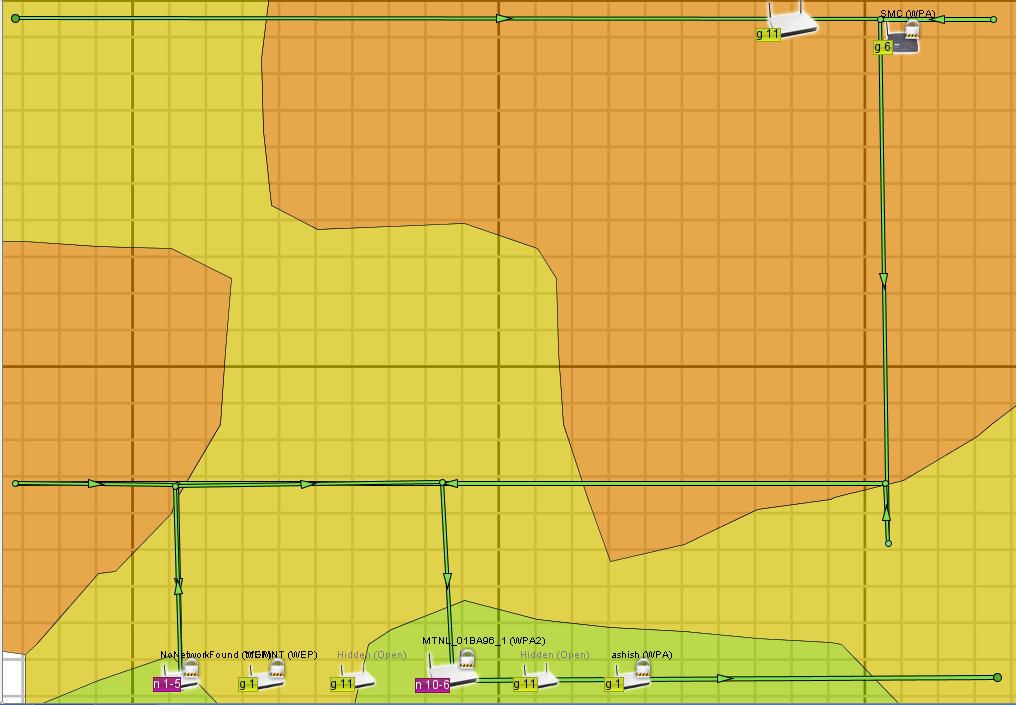
\includegraphics[scale=0.085]{./figures/ground_without_router.png}}
    \hspace{1mm}
    \subfloat[\scriptsize Ground floor WiFi Heatmap with additional router]{
    	 \label{fig:ground_with_router}
        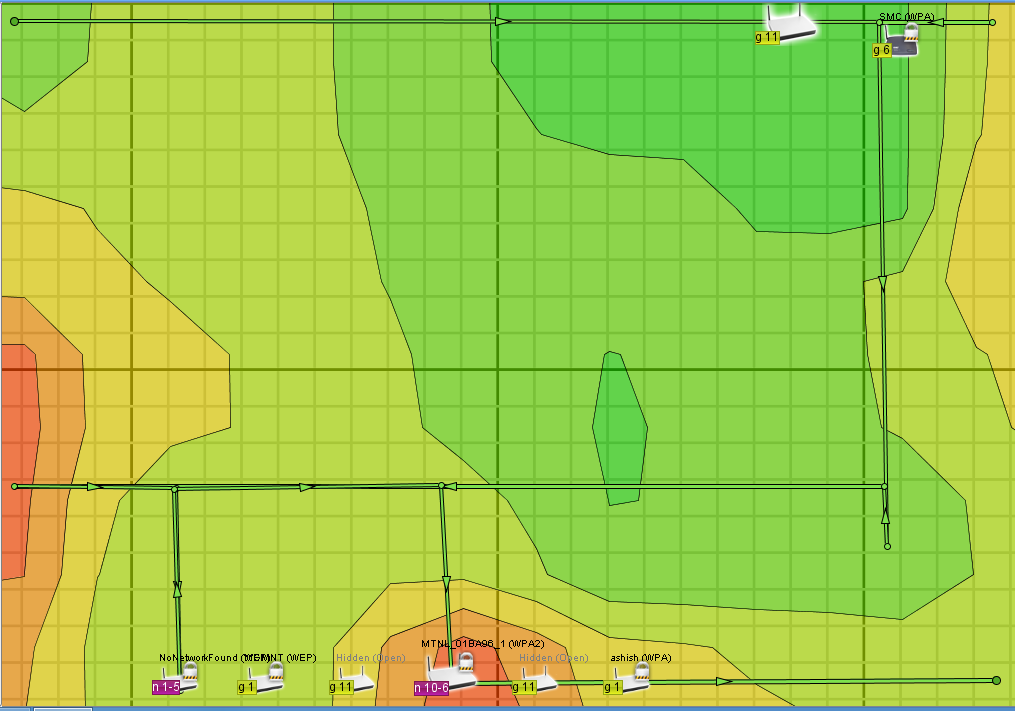
\includegraphics[scale=0.085]{./figures/ground_with_router.png}}
        \vspace{-3mm}
       \newline
      \subfloat[\scriptsize Second floor WiFi Heatmap without additional router]{
      	 \label{fig:second_without_router}
          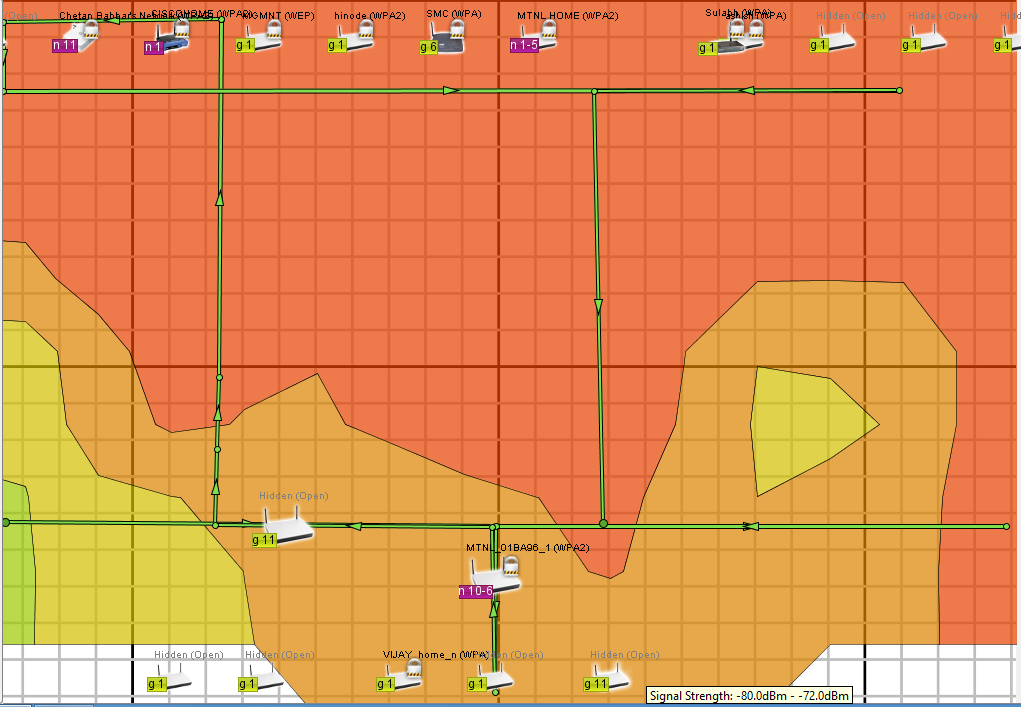
\includegraphics[scale=0.085]{./figures/without_.png}}
          \hspace{1mm}
          \subfloat[\scriptsize Second floor WiFi Heatmap with additional router]{
          	 \label{fig:second_with_router}
              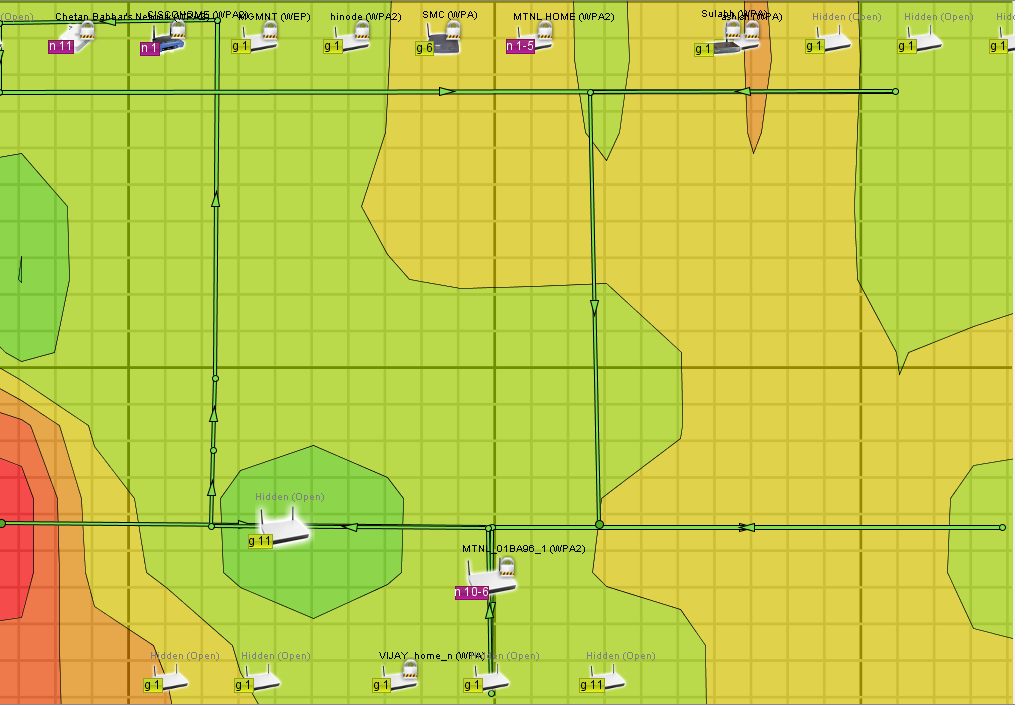
\includegraphics[scale=0.085]{./figures/with_.png}} 
    \caption{WiFi signal without placing additional routers on different floors is poor. The greener the region, the better the signal strength for the heatmap.}   
      
\end{figure}








\begin{figure}     
    \subfloat[\scriptsize Glowing LED's in night]{
        \label{fig:led}
        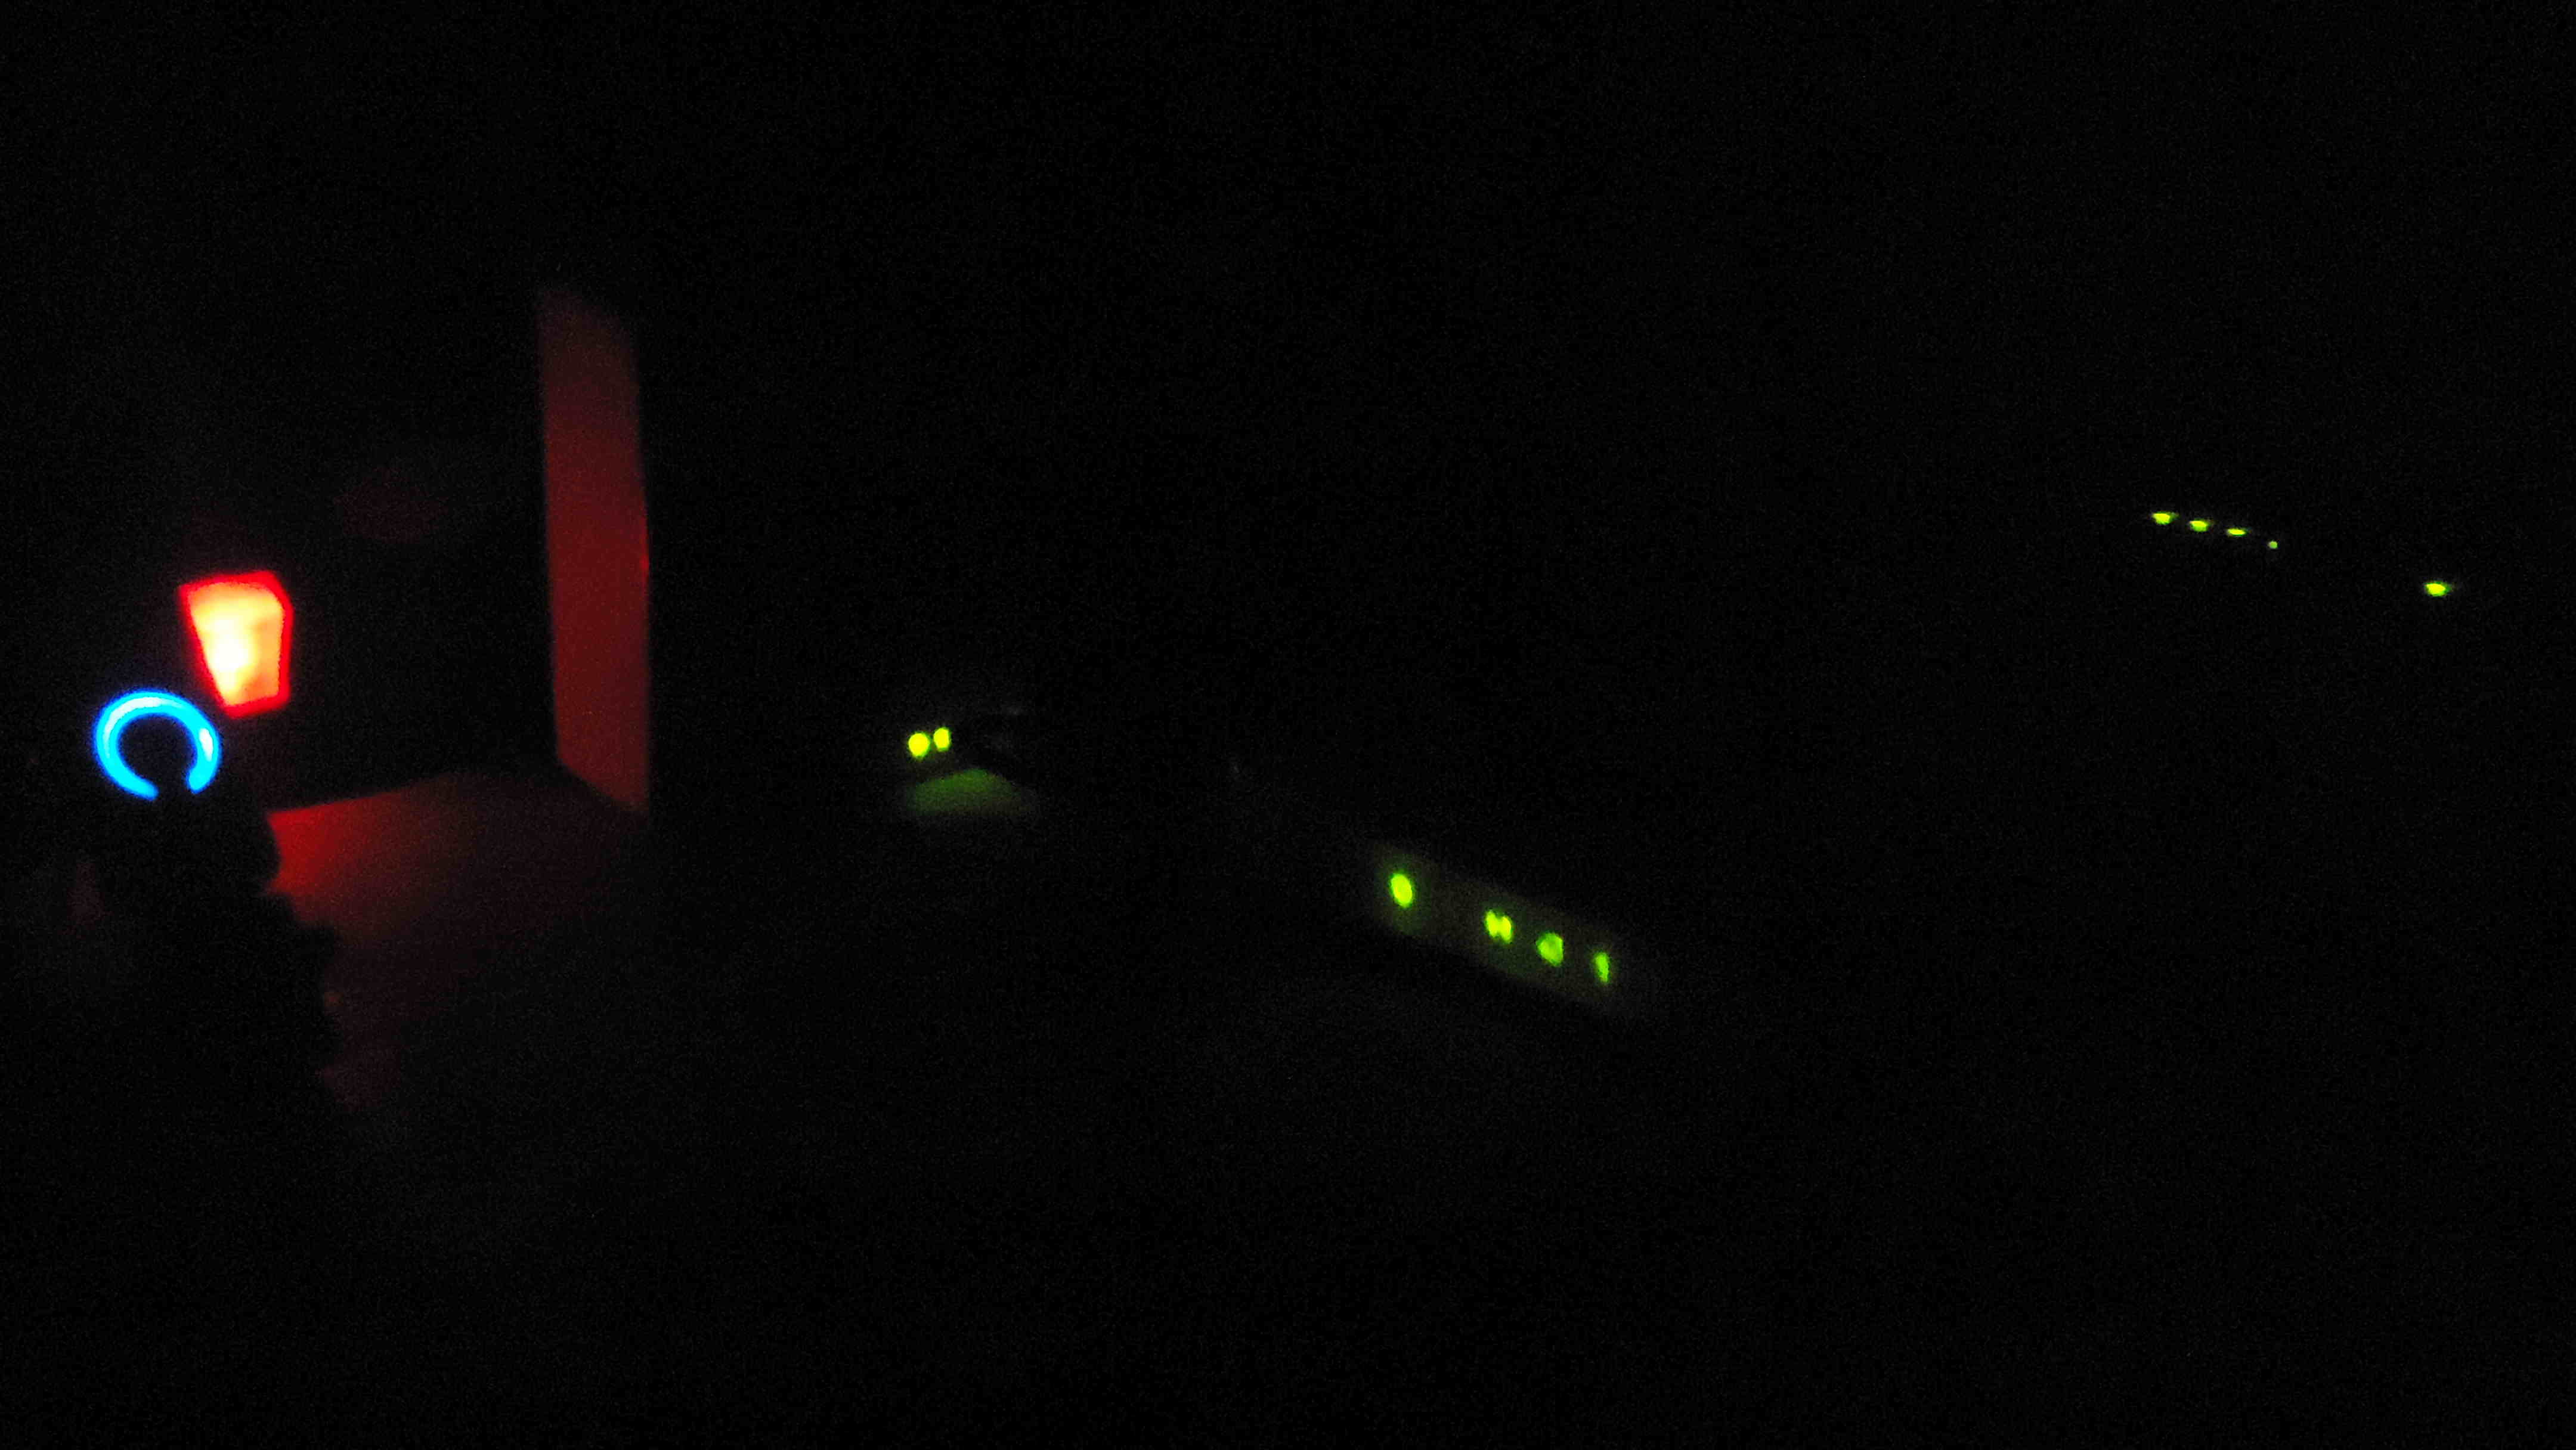
\includegraphics[scale=0.017]{./figures/led.jpg}}
        \hspace{0.02mm}
         \subfloat[\scriptsize Wire snag leading to data loss ]{
            \label{fig:snag}
            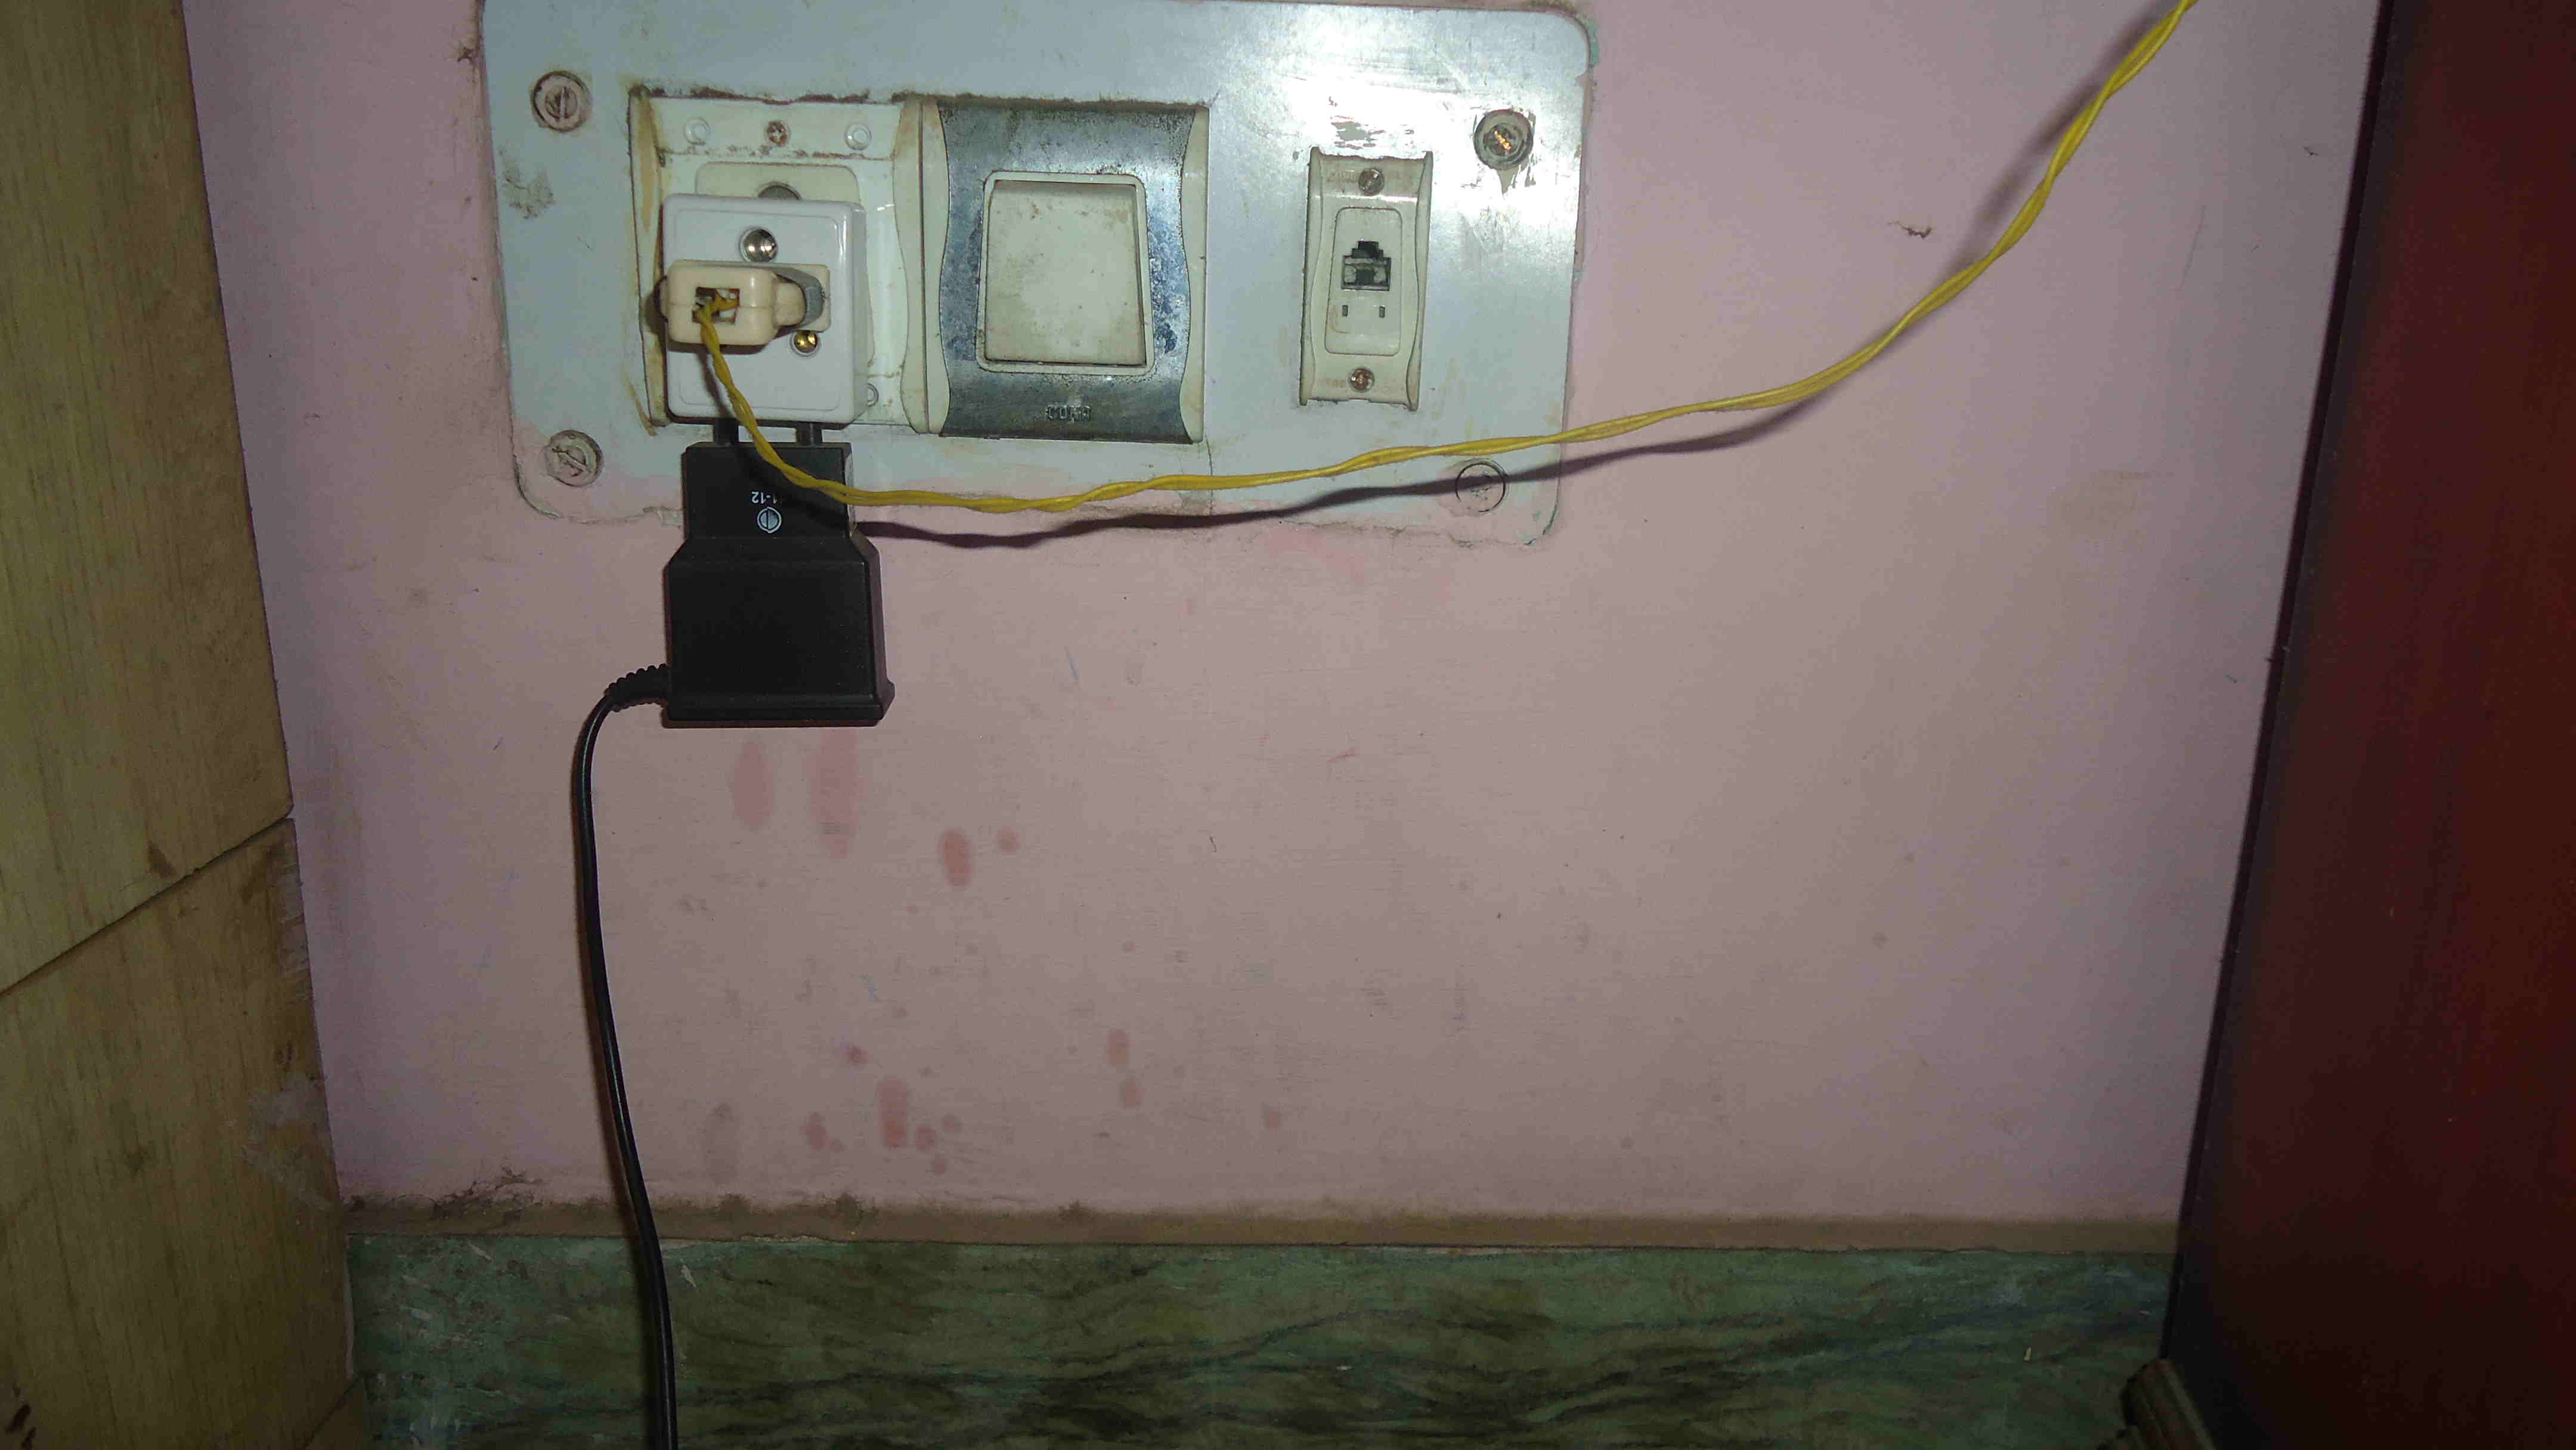
\includegraphics[scale=0.017]{./figures/snag.jpg}}
                    \hspace{0.02mm}
        \subfloat[\scriptsize Closely placed MCB's causing interference in CT monitroing circuit ]{
                    \label{fig:ct_interference}
                    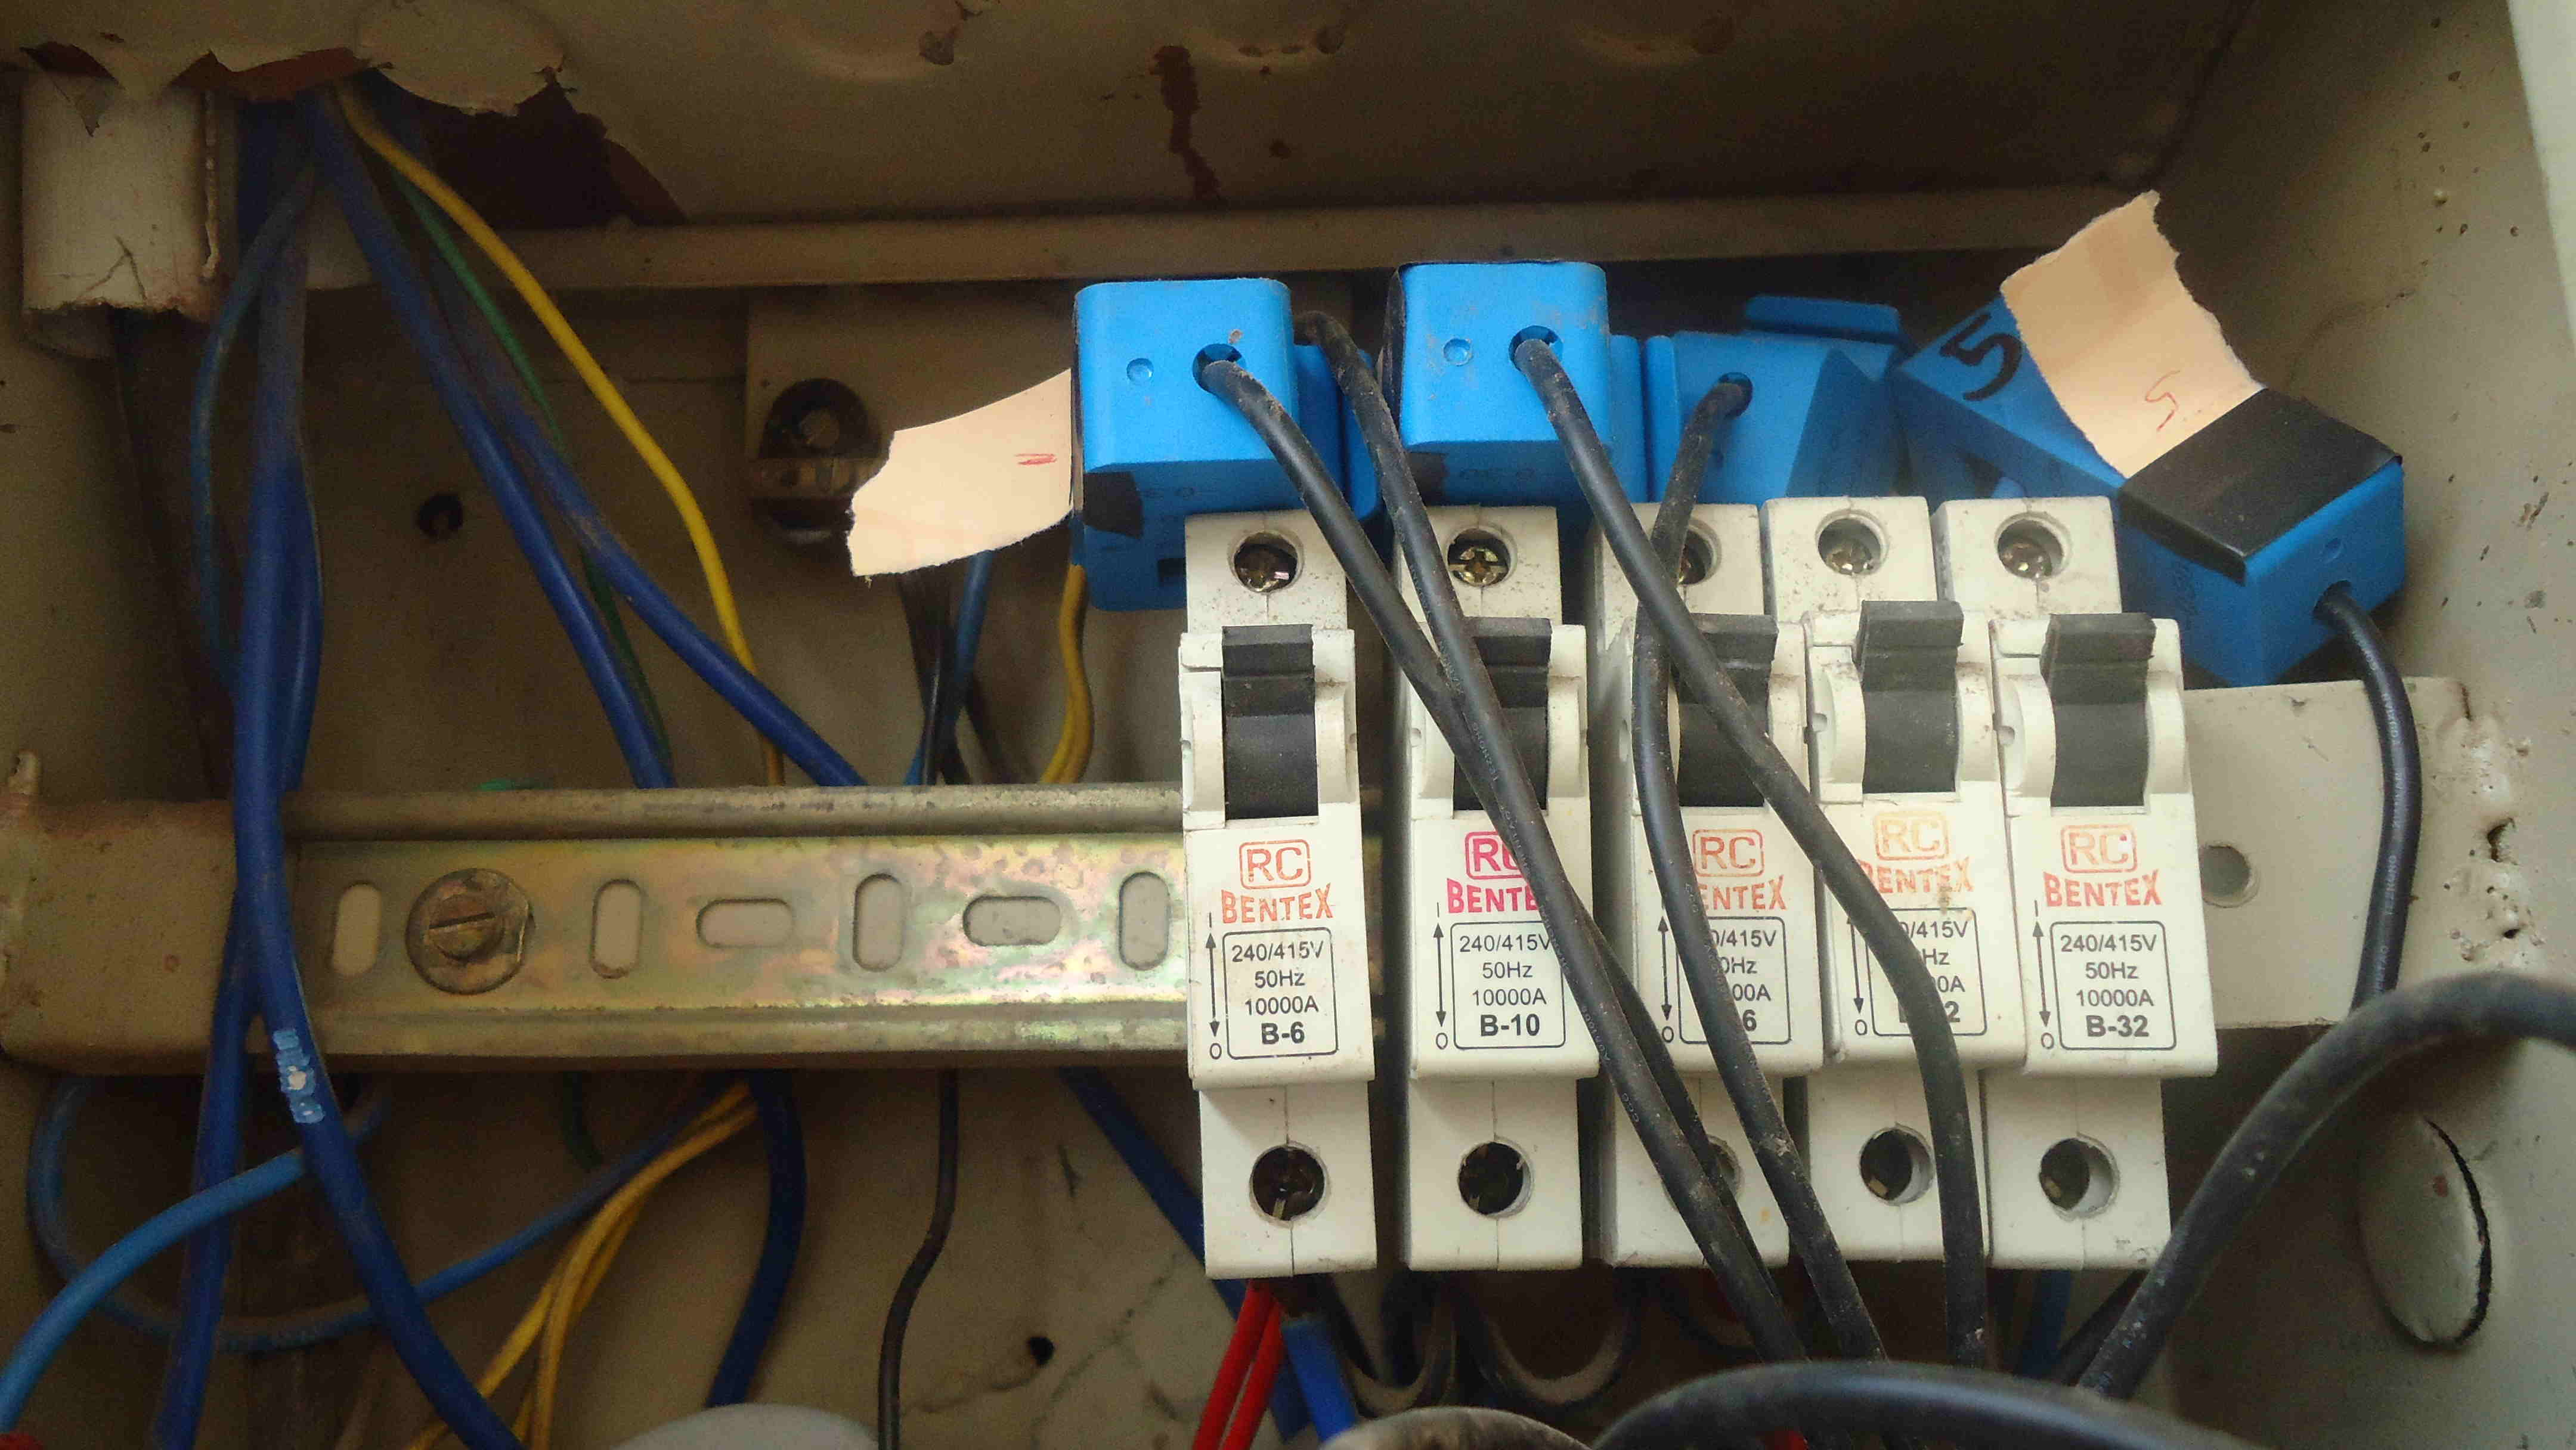
\includegraphics[scale=0.017]{./figures/ct_interference.jpg}}
    \caption{Common problems in residential deployments}   
    \label{fig:home}
   
\end{figure}


\section{Conclusions and Future Work}
In this paper, we present our experiences in an extensive residential deployment monitoring electrical, water and ambient parameters in Delhi, India. To the best of our knowledge, this is the first extensive residential deployment in a developing country. We present key differences between developing and developed countries, in terms of residential deployments. Some of these key differences are: unreliable nature of electrical grid, unreliable internet, different set and nature of electrical loads, concept of overhead water tanks. We verify residential deployments learnings presented in previous literature, such as poor wireless connectivity in homes and the importance of aesthetics.

Frequent power outages and unreliable internet motivated us to develop our sensing architecture: \paradigms, which accounts for these pitfalls by introducing local storage and periodic upload. Such architectures can be of particular importance in context of developing countries. 

We are in the process of installing our sensors across multiple faculty residences in our institute. We plan to carry out longer duration deployments which capture seasonal variations and after that we wish to release our data set in the public. We are also developing a billing application for providing detailed electricity usage information to home owners. We plan to perform NILM and provide the home occupants with detailed electricity consumption breakdown.
\balance
\bibliographystyle{abbrv}
\bibliography{references} 
\end{document}
